\documentclass{report}
% \includeonly{parts/0_notation, parts/1_basic_concepts, parts/2_number_sequences}
% \documentclass[11pt,a4paper]{article}

\input{preamble}
\input{macros}
\input{letterfonts}

% \addtolength{\textwidth}{130pt}
% \addtolength{\hoffset}{-2cm}
% \addtolength{\voffset}{-2cm}
% \addtolength{\textheight}{90pt}

% \tolerance=3000
% \def\baselinestretch{1.1}
% \flushbottom

% \parindent=1cm

\title{\textbf{HSE FCS SE}\\\textbf{Calculus-1 2023-2024}}
\author{Lecturer: Ivan Erlikh\\File edited by: vova kormilitsyn}
\date{
    \begin{flushright}
        ver. 1.3.2
    \end{flushright}
}

% \pagecolor{gray}
% \color{white}

\begin{document}

\maketitle

\tableofcontents

\chapter{Используемые обозначения}

\nt{
    $ \Nset $ - множество натуральных чисел. В данном файле полагаем, что $ 0 \notin \Nset $

    $ \Zset $ - множество целых чисел

    $ \Qset $ - множество рациональных чисел

    $ \Rset $ - множество вещественных чисел

    $ \Rset_{>0} $ - множество положительных вещественных чисел

    $ \ExtRset = \Rset \cup \{ +\infty; -\infty \} $ - дополненная прямая (extended real number line)

    $ \{ n, n + 1, ..., m \} $ - множество вещественных чисел от $n$ до $m$ "с шагом 1" включительно

    Формально, это множество равно $ \{ x \in \Rset | x \ge n \wedge x \le m \wedge x - n \in \Zset \}  $ 

    $ \circled{$\mathbb{W}$} $ - противоречие (используется при доказательстве методом от противного)

    (если Вам знаком символ $\bot$, то в данном файле полагаем эти обозначения эквивалентными)

    Через "$:=$" будем обозначать "положим по определению равным", например,
    $\forall \veps > 0:  \delta(\veps) := 2 \veps $ означает "для любого $\veps$, большего нуля, положим $\delta(\veps)$ равным $2 \veps$"

    Аббревиатурой БОО будем обозначать "без ограничения общности" 
    (возможно, Вам также знакомо выражение "не умаляя общности", в данном файле полагаем эти обозначения эквивалентными)

    $ C[a; b] $ - множество функций, непрерывных на отрезке $[a; b]$

    $ R[a; b] $ - множество функций, интегрируемых на отрезке $[a; b]$
}

\chapter{Логические операции}


\section{Высказывания, предикаты и кванторы}

\subsection{Определения}

\mcdfn{Высказывания и n-местные предикаты}
{
    Высказывание - это упрощённая модель повествования предложения,
    такая что каждое высказывание либо истинно, либо ложно, но не одновременно

    n-местные предикат (n-арный предикат) - это выражение, которое превращается в
    высказывание, если в нём заменить $ x_1, x_2, ..., x_n $ на подходящие имена, где
    $ x_1, x_2, ..., x_n $ - переменные в предикате
}

\mcdfn{Логические операции}
{
\begin{tabular}{rl}
    Отрицаниe:       & $\bullet$ $ \lnot A $ (также обозначают $ \overline{A} $) означает "не $A$" \\
    Логическое и:    & $\bullet$ $ A \wedge B $ означает "верно $A$ и верно $B$" \\
    Логическое или:  & $\bullet$ $ A \vee B $ означает "верно $A$, или верно $B$, или верны $A$ и $B$ вместе" \\
    Исключающее или: & $\bullet$ $ A \oplus B $ означает "верно ровно одно из высказываний $A$, $B$" \\
    Импликация:      & $\bullet$ $ A \implies B $ означает "если верно $A$, то верно $B$" \\
    Эквивалентность: & $\bullet$ $ A \iff B $ означает "$A$ верно тогда и только тогда, когда верно $B$" \\
\end{tabular}
}

\nt{
    Пусть $ A \implies B $

    Если $ A $ верно, то $ B $ тоже верно, но если $ A $ ложно, то $ B $ может быть и истинным, и ложным

    Пусть $ A \iff B $

    Если $ A $ ложно, то ложно $ B $. Если $ B $ верно, то верно $ A $
}

\nt
{
    Логические операции можно выражать через другие логические операции, например,

    $ (A \implies B) \iff (\lnot A \vee B) $
}

\mcdfn{Кванторы}
{
Квантор всеобщности обозначается как $ \forall $ и означает "для любого"

Квантор существования обозначается как $ \exists $ и означает "существует"

Квантор едиственности обозначается как $ ! $ и означает "едиственный, такой что ..."
}

\mcex{}
{
\begin{tabular}{rl}
    Всеобщность:    & $\bullet$ $ \forall x \in \Rset: \, \phi(x) $ означает \\
                    & "Для любого x из $\Rset $ выполняется предикат $ \phi(x) $" \\
    Существование:  & $\bullet$ $ \exists x \, (x \in \mathbb{Q} \implies \psi(x)) $ означает \\
                    & "Существует x, такой что если x из $\mathbb{Q} $, то выполняется предикат $ \psi(x) $" \\
    Единственность: & $\bullet$ $ \forall n \in \mathbb{N} \, \exists! k \in \mathbb{N} \cup \{ 0 \}: 2^k \le n < 2^{k + 1} $ означает \\
                    & "Для любого натурального числа существует и едиственно такое \\
                    & целое неотрицательное число $ k $, что $ 2^k \le n < 2^{k + 1} $" \\
\end{tabular}
}

\nt{
    На практике квантор едиственности часто используется вместе с квантором
    существования т.е. часто используют связку $ \exists! $, "существует и единственно"
}

\nt{
    Вместо "$\lnot \exists$" пишут "$\nexists$"
}

\subsection{Правило обращения кванторов}

\mcclm{Правило обращения кванторов}{}
{
    При обращении кванторов квантор существования
    меняется на квантор всеобщности, квантор всеобщности
    меняется на квантор существования, а утверждение под
    кванторами меняется на противоположное
}

\mcex{}
{
    Пусть дано высказывание:

    \[
    \forall n \in \mathbb{N} \,
    \exists m_1 \in \mathbb{Z} \,
    \exists m_2 > m_1 \,
    \forall q \in \mathbb{Q}: \,
        | m_1 | > n \wedge \lnot
        \psi(q \cdot m_1 \cdot m_2 - n)
    \]

    Тогда отрицание к этому высказыванию будет:
    \[
    \exists n \in \mathbb{N} \,
    \forall m_1 \in \mathbb{Z} \,
    \forall m_2 > m_1 \,
    \exists q \in \mathbb{Q}: \,
        | m_1 | \le n \vee
        \psi(q \cdot m_1 \cdot m_2 - n)
    \]
}

\section{Метод математической индукции}

\mcclm{Метод математической индукции}{}{
    Пусть есть предикат $ \phi(n) $, который выполняется или не выполняется при различных $ n \in \mathbb{N} $

    Тогда, если $ \exists k \in \mathbb{N}: \, \phi(k) $ и
    $ \forall n \ge k: (\phi(n) \implies \phi(n + 1)) $, то
    по методу математической индукции получаем $ \forall n \ge k: \phi(n) $

    Этапы доказательства:

\begin{tabular}{rl}
    База индукции:          & $\bullet$ Проверка истинности $ \phi(k) $ \\
    Предположение индукции: & $\bullet$ Пусть для некоторого $ n \in \mathbb{N} \wedge n \ge k $ верно $ \phi(n) $ \\
    Шаг индукции:           & $\bullet$ Докажем, что $ \phi(n + 1) $, используя предположение индукции \\
    Вывод:                  & $\bullet$ $ \forall n \ge k: \phi(n) $ \\
\end{tabular}
}

\section{Неравенство Бернулли}

\mcthm{Неравенство Бернулли}{
    Если $ n \in \mathbb{N} $ и $ x \ge -1 $, то $ (1 + x)^n \ge 1 + xn $
\mcprf{
\begin{split}
    & \text{Докажем неравенство при помощи метода математической индукции} \\
    & \text{1. База индукции:} \\
    & \text{Пусть } n = 1 \implies (1 + x)^n = 1 + x \ge 1 + x \\
    & \text{2. Предположение индукции:} \\
    & \text{Пусть для некоторого } n \ge 1 \text{ верно, что } (1 + x)^n \ge 1 + xn \\
    & \text{3. Шаг индукции: Рассмотрим неравенство, подставив в него } n + 1: \\
    & (1 + x)^{n+1} = (1 + x)^n \cdot (1 + x) \\
    & 1 + x \ge 0 \implies (1 + x)^n \cdot (1 + x) \ge (1 + xn) \cdot (1 + x) = 1 + xn + x + n \cdot x^2 \ge 1 + nx + x = 1 + n(x + 1) \\
    & \text{Следовательно, } (1 + x)^{n+1} \ge 1 + n(x + 1) \\
    & \text{4. Обозначим доказываемое как предикат } \phi(n) \text{, тогда получаем:} \\
    & \phi(1) \wedge \forall n \in \mathbb{N}: (\phi(n) \implies \phi(n + 1)) \\
    & \text{Тогда по принципу математической индукции } \forall n \in \mathbb{N}: \phi(n) \\
\end{split}
}
}

\section{Перестановки, размещения, сочетания}

\mcdfn{Перестановки, размещения и сочетания}
{
    Пусть дано множество из $n$ элементов

    $\bullet$ Если все элементы попарно различны (т.е. при решении задачи мы считаем, что два любых элемента множества различны),
    то количество попарно различных перестановок этого множества обозначается как $ P_n $ и равно $ n! $

    Пусть зафиксировано $ k \in \mathbb{N} \cup \{ 0 \} $, такое что $ k \le n $, тогда:

    $\bullet$ Количество количество способов, которыми мы можем выбрать
    $k$-элементное подмножество данного множества, считая, что элементы попарно различны, 
    обозначается как $A_n^k$ и равно $\frac{n!}{(n - k)!}$

    $\bullet$ Количество количество способов, которыми мы можем выбрать
    $k$-элементное подмножество данного множества, считая, что все элементы попарно равны, 
    обозначается как $C_n^k$ и равно $\frac{n!}{k! (n - k)!}$
}

\nt{
    Пусть есть есть конечная последовательность из $ n $ натуральных чисел от 1 до $n$ (кортеж из $n$ элементов от $1$ до $n$)

    Тогда количество различных перестановок элементов кортежа равно $ P_n = n! $

    Количество способов выбрать $k$ чисел из кортежа, считая их перестановки различными, равно $ A_n^k = \frac{n!}{(n - k)!} $

    Количество способов выбрать $k$ чисел из кортежа, считая, что все перестановки одного набора - это один способ, равно $ C_n^k = \frac{n!}{k! (n - k)!} $

    Пусть $ \sigma = (1, 2, 3, 4) $ - данный кортеж, тогда есть $P_4 = 24$ различных перестановок $ \sigma $:
\begin{equation*}
\begin{split}
    & (1, 2, 3, 4), (1, 2, 4, 3), (1, 3, 2, 4), (1, 3, 4, 2), (1, 4, 2, 3), (1, 4, 3, 2) \\
    & (2, 1, 2, 4), (2, 1, 4, 2), (2, 3, 1, 4), (2, 3, 4, 1), (2, 4, 1, 3), (2, 4, 3, 1) \\
    & (3, 1, 2, 4), (3, 1, 4, 2), (3, 2, 1, 4), (3, 2, 4, 1), (3, 4, 1, 2), (3, 4, 2, 1) \\
    & (4, 1, 2, 3), (4, 1, 3, 2), (4, 2, 1, 3), (4, 2, 3, 1), (4, 3, 1, 2), (4, 3, 2, 1) \\
\end{split}    
\end{equation*}

    Для $k = 2$ есть $A_4^2 = 12 $ способ выбрать кортеж из 2 элементов:
\begin{equation*}
\begin{split}
    & (1, 2), (1, 3), (1, 4), (2, 1), (2, 3), (2, 4) \\
    & (3, 1), (3, 2), (3, 4), (4, 1), (4, 2), (4, 3) \\
\end{split}    
\end{equation*}

    Для $k = 2$ есть $C_4^2 = 6 $ способ выбрать подмножество из 2 элементов (порядок элементов не важен):
\begin{equation*}
\begin{split}
    & (1, 2), (1, 3), (1, 4), (2, 3), (2, 4), (3, 4) \\
\end{split}    
\end{equation*}
}

\section{Бином Ньютона}

\mcthm{Бином Ньютона}
{
    $ (a + b)^n = \sum_{k = 0}^{n} \Cmb{n}{k} a^{k} b ^ {n-k}
    (\text{формально, перед равенством необходимо написать }
        \forall a, b \in \Rset \forall n \in \mathbb{N}) $
\begin{mcproof}
\begin{equation*}
\begin{split}
& \text{Докажем это утверждение при помощи метода математической индукции} \\
& \text{1. База индукции: } n = 1 \implies (a + b)^n = a + b = \sum_{k=0}^{1} \Cmb{n}{k} a^k b^{n-k} \\
& \text{2. Предположение индукции: пусть для некоторого } n \ge 1: (a + b)^{n}= \sum_{k = 0}^{n} \Cmb{n}{k} a^{k} b ^ {n-k} \\
& \text{3. Рассмотрим равенство и докажем, что оно верно при подстановке } n + 1: \\
& (a + b)^{n + 1}
    = (a + b) (a + b)^n
    = (a + b) \sum_{k = 0}^{n} \Cmb{n}{k} a^{k} b ^ {n-k} = \\
&   = a \sum_{k = 0}^{n} \Cmb{n}{k} a^{k} b ^ {n - k}
        + b \sum_{k = 0}^{n} \Cmb{n}{k} a^{k} b ^ {n - k}
    = \sum_{k = 0}^{n} \Cmb{n}{k} a^{k + 1} b ^ {n - k}
        + \sum_{k = 0}^{n} \Cmb{n}{k} a^{k} b ^ {n + 1 - k} \\
&   = \sum_{k = 1}^{n + 1} \Cmb{n}{k - 1} a^{k} b ^ {n - (k - 1)}
        + \sum_{k = 0}^{n} \Cmb{n}{k} a^{k} b ^ {n + 1 - k}
    = \Cmb{n}{n} a^{n + 1} b^0 + \sum_{k = 1}^{n} \Cmb{n}{k - 1} a^{k} b ^ {n + 1 - k}
        + \Cmb{n}{0} a^{0} b^{n + 1} \sum_{k = 1}^{n} \Cmb{n}{k} a^{k} b ^ {n + 1 - k} = \\
&   = a^{n + 1} + b^{n + 1}
        + \sum_{k = 1}^{n} (\Cmb{n}{k - 1} + \Cmb{n}{k}) a^{k} b ^ {n + 1 - k}
    = \Cmb{n + 1}{n + 1} a^{n + 1} + \Cmb{n + 1}{0} b^{n + 1}
        + \sum_{k = 1}^{n} \Cmb{n + 1}{k} a^{k} b ^ {n + 1 - k} = \\
&   = \sum_{k = 0}^{n + 1} \Cmb{n + 1}{k} a^{k} b ^ {n + 1 - k} \\
& \text{4. Получили: } \\
& \text{Равенство верно при $n = 1$,
    а из верности равенства для $ n $ следует верность равенства для $ n + 1 $} \\
& \text{(при $ n \ge 1 $), тогда по методу математической индукции получим, что равенство верно $ \forall n \in \mathbb{N} $} \\
\end{split}
\end{equation*}
\end{mcproof}
}

\chapter{Определения и свойства числовых последовательностей}

\section{Определения}

\subsection{Числовая последовательность}

\mcdfn{Числовая последовательность}
{
    Числовая последовательность - это счётно бесконечный проиндексированный набор чисел
}

\mcclarf{Уточнение}{
    Формально, числовая последовательность (далее обозначается ч.п.) - это функция натурального аргумента

    $ f: \mathbb{N} \to \Rset$

    Способы задания:
\begin{tabular}{rl}
    & $\bullet$ Формула. Например, $ a_n = \left(1 + \frac{1}{n}\right)^n $ \\
    & $\bullet$ Рекуррентно. Например, $ F_n = F_{n - 1} + F_{n - 2} $ \\
\end{tabular}
}

\subsection{Определения монотонных числовых последовательностей}

\mcdfn{Монотонность ч.п.}
{
    Ч.п. $ \NumSeq{a_n} $ называется строго возрастающей, если $ \forall n \in \mathbb{N}: a_{n + 1} > a_{n} $

    Ч.п. $ \NumSeq{a_n} $ называется строго убывающей, если $ \forall n \in \mathbb{N}: a_{n + 1} < a_{n} $

    Ч.п. $ \{ a_n \} $ называется неубывающей, если $ \forall n \in \mathbb{N}: a_{n + 1} \ge a_{n} $

    Ч.п. $ \{ a_n \} $ называется невозрастающей, если $ \forall n \in \mathbb{N}: a_{n + 1} \le a_{n} $
}


\subsection{Ограниченная ч.п.}

\mcdfn{Ограниченная сверху числовая последовательность}
{
    Числовая последовательность $ \NumSeq{a_n} $ называется ограниченной сверху, если

    $ \exists C \in \Rset \, \forall n \in \mathbb{N}: \, a_n < C $
}

\mcdfn{Ограниченная снизу числовая последовательность}
{
    Числовая последовательность $ \NumSeq{a_n} $ называется ограниченной снизу, если

    $ \exists C \in \Rset \, \forall n \in \mathbb{N}: \, a_n > -C $
}

\mcdfn{Ограниченная числовая последовательность}
{
    Числовая последовательность $ \NumSeq{a_n} $ называется ограниченной, если

    $ \exists C > 0 \, \forall n \in \mathbb{N}: \, | a_n | < C $
}

\mcex{}{
    Пример: $ a_n = 5 + \frac{1}{n} $

    $ \exists C = 7 > 0 \, \forall n \in \mathbb{N}: \, | a_n | = \left| 5 + \frac{1}{n} \right| < 7 = C $
}

\nt
{
    Числовая последовательность ограничена $ \iff $ она ограничена сверху и ограничена снизу
}

\subsection{Неограниченная ч.п.}

\mcdfn{Неограниченная числовая последовательность}
{
    Числовая последовательность $ \NumSeq{a_n} $ называется неограниченной, если она не является ограниченной, то есть

    $ \forall C > 0 \, \exists n \in \mathbb{N}: \, | a_n | \ge C $
}

\mcex{}{
    Пример: $ a_n = n $

    $ \forall C > 0 \, \exists n = \left\lceil C \right\rceil \in \mathbb{N}: \, | a_n | \ge C $
}

\subsection{Отделимая от нуля ч.п.}

\mcdfn{Отделимая от нуля числовая последовательность}
{
    Числовая последовательность $ \NumSeq{a_n} $ называется отделимой от нуля, если

    $ \exists \veps > 0 \, \forall n \in \mathbb{N}: \, | a_n | > \veps $
}

\mcex{}{
    Пример: $ a_n = 2 - \frac{1}{n} $

    $ \exists \veps = 0.5 > 0 \, \forall n \in \mathbb{N}: \, \left| a_n \right| = \left| 2 - \frac{1}{n} \right| > 0.5 = \veps $
}

\subsection{Сходящаяся ч.п.}

\mcdfn{Сходящаяся числовая последовательность}
{
    Числовая последовательность называется сходящейся, если она имеет конечный предел при $ n \to +\infty $, т.е.
    ч.п. $ \NumSeq{a_n} $ называется сходящейся, если:

    \[ \exists A \in \Rset \, \forall \veps > 0 \, \exists N = N(\veps) \in \mathbb{N} \, \forall n > N: | a_n - A | < \veps \]

    Обозначение:
    \[ \lim_{n \to +\infty} a_n = A, A \in \Rset \]
}

\mcex{}{
\begin{equation*}
\begin{split}
    & \text{Пример: } a_n = \frac{4 n^3 + 2 n^2 + 1}{2 n^3 + 1} \\
    & \text{Докажем, что  } \lim_{n \to +\infty} a_n = 2 = A \\
    & \text{Пусть $\veps > 0$, тогда:} \\
    & | a_n - 2 | < \veps 
        \impliedby \left| \frac{4 n^3 + 2 n^2 + 1}{2 n^3 + 1} - 2 \right| < \veps 
        \impliedby \left| \frac{2 n^2 - 1}{2 n^3 + 1} \right| < \veps \impliedby \\
    & \impliedby \frac{2 n^2 - 1}{2 n^3 + 1} < \veps 
        \impliedby \frac{2 n^2}{2 n^3 + 1} < \veps
        \impliedby \frac{2 n^2}{2 n^3} < \veps
        \impliedby \frac{1}{n} < \veps
        \impliedby \frac{1}{\veps} < n \\
    & \text{Тогда:} \\
    & \forall \veps > 0 \, \exists N = N(\veps) = \left\lceil \frac{1}{\veps} \right\rceil \, \forall n > N \ge \frac{1}{\veps}: | a_n - 2 | < \veps \\
\end{split}
\end{equation*}
}

\nt{
    Сходящаяся ч.п. является ограниченной
}

\subsection{Эпсилон окрестность}

\mcdfn{Эпсилон окрестность}
{
    Эпсилон окрестностью вещественного числа $ x_0 $ (элемента поля вещественных чисел)
    называется множество $ (x_0 - \veps; x_0 + \veps) $ и обозначается $ U_{\veps}(x_0) $.

    Обычно говорят "Эпсилон окрестность точки $ x_0 $"
}

\mcex{}{
    $ U_1(\pi) = (\pi - 1; \pi + 1) $

    $ U_e(e) = (0; 2 e) $
}

\mcdfn{Проколотая эпсилон окрестность}
{
    Проколотой эпсилон окрестностью вещественного числа $ x_0 $ (элемента поля вещественных чисел)
    называется множество $ (x_0 - \veps; x_0 + \veps) \setminus \{ x_0 \} $ и обозначается $ \dot{U}_{\veps}(x_0) $.

    Обычно говорят "Проколотая эпсилон окрестность точки $ x_0 $"
}

\mcex{}{
    $ \dot{U}_1(e) = (e - 1; e + 1) \setminus \{ e \} = (e - 1; e) \cup (e; e + 1) $
}

\nt{
    Неравенство $ | a_n - A | < \veps $ равносильно тому, что $ a_n \in U_\veps(A) $
}

\subsection{Бесконечно большая ч.п.}

\mcdfn{Бесконечно большая числовая последовательность}
{
    Числовая последовательность $ \NumSeq{a_n} $ называется бесконечно большой, если она стремится к $ +\infty$, к $ -\infty $ или к $ \infty $ при $ n \to +\infty $, т.е.

\begin{tabular}{rl}
    & $\bullet$
        $ \lim_{n \to +\infty} a_n = +\infty \iff
        \forall M > 0 \, \exists N = N(M) \forall n > N: a_n > M $ \\
    & $\bullet$
        $ \lim_{n \to +\infty} a_n = -\infty \iff
        \forall M > 0 \, \exists N = N(M) \forall n > N: a_n < -M $ \\
    & $\bullet$
        $ \lim_{n \to +\infty} a_n = \infty \iff
        \forall M > 0 \, \exists N = N(M) \forall n > N: | a_n | > M $ \\
\end{tabular}
}

\mcex{}{
    Пример б.б. ч.п., стремящейся к $ +\infty $: $ a_n = n $

    Пример б.б. ч.п., стремящейся к $ -\infty $: $ a_n = -n $

    Пример б.б. ч.п., стремящейся к $ \infty $: $ a_n = (-1)^n \cdot n $
}

\subsection{Бесконечно малая ч.п.}

\mcdfn{Бесконечно малая числовая последовательность}
{
    Числовая последовательность $ \NumSeq{a_n} $ называется бесконечно малой, если она стремится к 0 при $ n \to +\infty $, т.е.

    $ \forall \veps > 0 \exists N = N(\veps) \forall n > N: | a_n | < \veps $
}

\section{Связи числовых последовательностей}

\nt{
\begin{tabular}{rl}
    Связи числовых последовательностей:

    & $\bullet$ $ \frac{1}{\text{б.б.}} = \text{б.м.} $ \\
    & $\bullet$ $ \frac{1}{\text{б.м.}} = \text{б.б.} $ \\
    & $\bullet$ $ \frac{1}{\text{ограниченная}} = \text{отделимая от нуля} $ \\
    & $\bullet$ $ \frac{1}{\text{отделимая от нуля}} = \text{ограниченная} $ \\
\end{tabular}
}

\nt
{
    Если ч.п. сходится или является б.б., то предел единственный
}

\mcprop{Докажите по определению, что}
{
    (ограниченная ч.п.) + (ограниченная ч.п.) = ограниченная ч.п.

    б.м + б.м. = б.м.

    б.м. $\cdot$ (ограниченная ч.п.) = б.м.

    $\frac{\text{отделимая от нуля ч.п.}}{\text{ограниченная ч.п.}}$ = ограничена ч.п.
}

\mcprop{Приведите пример, когда}
{
    (отделимая от нуля ч.п.) + (отделимая от нуля ч.п.) = отделимая от нуля ч.п.

    (отделимая от нуля ч.п.) + (отделимая от нуля ч.п.) = б.м.

    б.б + б.б = б.б.

    б.б + б.б = б.м.

    б.б + б.б = (ограниченная ч.п.)

    б.б + б.б = (отделимая от нуля ч.п.)
}

% TODO: check
\pagebreak
\section{Арифметика предела ч.п.}

\mcclm{}{}{
    Если $ a_n \underset{n \to +\infty}{\to} a, b_n \underset{n \to +\infty}{\to} b $, то

\begin{tabular}{rl}
    \\
    & $\bullet$ $ a_n \pm b_n \underset{n \to +\infty}{\to} a \pm b $ \\
    \\
    & $\bullet$ $ a_n \cdot b_n \underset{n \to +\infty}{\to} a \cdot b $ \\
    \\
    & $\bullet$ $ b \ne 0 \wedge \forall n \in \mathbb{N} \implies b_n \ne 0: \frac{a_n}{b_n} \underset{n \to +\infty}{\to} \frac{a}{b}  $ \\
    \\
    & $\bullet$ $ \forall n \in \mathbb{N}: a_n \ge 0 \implies \sqrt[]{a_n} \underset{n \to +\infty}{\to} \sqrt[]{a} $ \\
\end{tabular}
}

\section{Теоремы}

\subsection{Теорема о предельном переходе в неравенствах}

\mcthm{Теорема: свойство предельного перехода в неравенствах}
{
    \[ (\exists N \in \mathbb{N} \, \forall n \ge N: c_n > A) \wedge (\lim_{n\to\infty} c_n = C) \implies C \ge A \]

    То есть если начиная с некоторого номера все члены последовательности $ > A $, 
    и сама последовательность сходится к $ C \in \Rset $ при $ n \to +\infty $, 
    то $ C \ge A $

\mcprf{
\begin{split}
    & \text{1. Распишем, что дано, по определению:} \\
    & \forall \veps > 0 \exists N_1(\veps) \forall n > N_1(\veps): | c_n - C | < \veps \\
    & \text{Это равносильно } \forall \veps > 0 \exists N_1(\veps) \forall n > N_1(\veps): C - \veps < c_n < C + \veps \\
    & \exists N \in \mathbb{N} \, \forall n \ge N: c_n > A \\
    & \text{2. Для любого $ \veps $ рассмотрим } M(\veps) = \max(N_1(\veps), N) + 1 \\
    & \text{Тогда } \forall \veps > 0 \exists M(\veps) = \max(N_1(\veps), N) + 1 \, \forall n > M: (C - \veps < c_n < C + \veps \wedge c_n > A) \\
    & \text{Следовательно, } \forall \veps > 0 \exists M(\veps) \, \forall n > M: C + \veps > A \\
    & \text{Выражение под кванторами не зависит от $M$ и $n$ } \implies \forall \veps > 0: C + \veps > A \\
    & \text{3. Предположим от противного, что } C < A \\
    & \text{Положим } \veps := \frac{A - C}{2} > 0 \implies C + \veps = C + \frac{A - C}{2} = \frac{A + C}{2} < A \\
    & \text{Получили, что }
        \exists \veps > 0: C + \veps < A
        \implies \circled{$\mathbb{W}$} \implies \text{ предположение, что $ C < A $, неверно}
        \implies C \ge A \\ 
\end{split}
}
}

\subsection{Теорема о зажатой последовательности}

\mcthm{Теорема о зажатой последовательности (о 2 миллиционерах / 2 полицейских / гамбургерах)}
{
\begin{minipage}[t]{\textwidth}
$$
\left. \begin{tabular}{l}
    $ a_n, b_n, c_n $ - числовые последовательности \\
    $ \lim_{n\to\infty} a_n = X $ \\
    $ \lim_{n\to\infty} b_n = X $ \\
    $ \exists N \in \mathbb{N} \hspace{2pt} \forall n \ge N: a_n \le c_n \le b_n $
\end{tabular} \right\}
\begin{tabular}{l}
    $ \implies \lim_{n\to\infty} c_n = X $
\end{tabular}
$$
\end{minipage}
\begin{mcproof}
\begin{equation*}
\begin{split}
    & \text{Докажем для случая, когда } X \in \Rset
        \text{. При } X \in \ExtRset \setminus \Rset
        \text{ доказательство проводится аналогично} \\
    & \text{1. Распишем по определению пределы.} \\
    & \forall \veps > 0 \, \exists N_1(\veps) \, \forall n > N_1(\veps): X - \veps < a_n < X + \veps \\
    & \forall \veps > 0 \, \exists N_2(\veps) \, \forall n > N_2(\veps): X - \veps < b_n < X + \veps \\
    & \text{Рассмотрим } N_3(\veps) = \max(N_1(\veps), N_2(\veps), N) \text{, тогда } \\
    & \forall \veps > 0 \, \exists N_3(\veps) \, \forall n > N_3(\veps): X - \veps < a_n \le c_n \le b_n < X + \veps \\
    & \implies \forall \veps > 0 \, \exists N_3(\veps) \, \forall n > N_3(\veps): X - \veps < c_n < X + \veps \\
\end{split}
\end{equation*}
\end{mcproof}
}

\subsection{Свойство предела б.м. ч.п.}

\mcthm{Свойство предела б.м. ч.п.}
{
    если $ a \in \Rset $, то \[\lim_{n\to\infty} a_n = a \iff a_n = a + \alpha_n, \text{где } \alpha_n \text{ - б.м. ч.п.} \]
\mcprf{
\begin{split}
    & "\implies" \\
    & \text{Распишем по определению, что дано:} \\
    & \lim_{n\to\infty} a_n = a \iff \forall \veps > 0 \, \exists N(\veps) \, \forall n > N(\veps): | a_n - a | < \veps \\
    & \text{Обозначим ч.п. } \alpha_n = a_n - a \text{, тогда } a_n = a + \alpha_n \\
    & \text{Тогда: } \forall \veps > 0 \, \exists N(\veps) \, \forall n > N(\veps): | \alpha_n | < \veps \\
    & \text{Доказали, что } a_n = a + \alpha_n \text{, где } \alpha_n \text{ - б.м. ч.п.} \\
    & "\impliedby" \\
    & \text{Распишем то, что $ \alpha_n $ - б.м., по определению:} \\
    & \lim_{n\to\infty} a_n = a \iff \forall \veps > 0 \, \exists N(\veps) \, \forall n > N(\veps): | \alpha_n | < \veps \\
    & \text{По условию } a_n = a + \alpha_n \text{, тогда } a_n - a = \alpha_n \text{, подставим в выражение под кванторами:} \\
    & \forall \veps > 0 \, \exists N(\veps) \, \forall n > N(\veps): | a_n - a | < \veps \\
    & \text{Доказали по определению, что } \lim_{n\to\infty} a_n = a \\
\end{split}
}
}

\chapter{Элементы теории множеств}

\section{Аксиома непрерывности}

\mcclm{Аксиома непрерывности действительных чисел (принцип полноты)}{}
{
$$
\left. \begin{tabular}{l}
    $ A \subseteq \mathbb{R} $ \\
    $ A \ne \varnothing $ \\
    $ B \subseteq \mathbb{R} $ \\
    $ B \ne \varnothing $ \\
    $ \forall a \in A \, \forall b \in B: a \le b $
\end{tabular} \right\}
\begin{tabular}{l}
    $ \implies \exists c \in \mathbb{R} \, \forall a \in A \, \forall b \in B: a \le c \le b $
\end{tabular}
$$
}

\section{Определения ограниченных множеств}

\mcdfn{Ограниченное сверху множество}
{
    Подможество $ A \subseteq \mathbb{R} $ называется ограниченным
    свеху, если
    $ \exists C \in \mathbb{R} \,
        \forall a \in A: \, a \le C $
}

\mcdfn{Ограниченное снизу множество}
{
    Подможество $ A \subseteq \mathbb{R} $ называется ограниченным
    снизу, если
    $ \exists C \in \mathbb{R} \,
        \forall a \in A: \, a \ge C $
}

\mcdfn{Ограниченное множество}
{
    Подможество $ A \subseteq \mathbb{R} $ называется ограниченным, если
    $ \exists C > 0 \,
        \forall a \in A: \, | a | \le C $
}

\section{Определения граней множества}

\mcdfn{Определение верхней грани множества}{
    Пусть дано множество $ A \subset \mathbb{R} \wedge A \ne \varnothing $.
    Тогда верхней гранью множества $ A $ называют число $ c \in \mathbb{R} $, такое что
    $ \forall a \in A: a \le c $
}

\mcdfn{Определение нижней грани множества}{
    Пусть дано множество $ A \subset \mathbb{R} \wedge A \ne \varnothing $.
    Тогда нижней гранью множества $ A $ называют число $ c \in \mathbb{R} $, такое что
    $ \forall a \in A: a \ge c $
}

\mcdfn{Определение точной верхней грани множества}{
    Пусть дано множество $ A \subset \mathbb{R} \wedge A \ne \varnothing $.
    Тогда точной верхней гранью множества $ A $ называют наименьший элемента множества
    всех верхних граней множества $ A $ и обозначают $ \sup A $
}

\mcdfn{Определение точной нижней грани множества}{
    Пусть дано множество $ A \subset \mathbb{R} \wedge A \ne \varnothing $.
    Тогда точной нижней гранью множества $ A $ называют наибольший элемента множества
    всех нижней граней множества $ A $ и обозначают $ \inf A $
}

\nt{
    Вообще говоря, наименьшый и наибольший элементы множества не всегда существуют. \\
    Например, у множества $(0; 1)$ нет ни наименьшего, ни наибольшего элементов, при этом \\
    $ \sup (0; 1) = 1 \notin (0; 1) $, $ \inf (0; 1) = 0 \notin (0; 1) $
}

\section{Теорема о существовании точной грани множества}

\mcthm{Теорема о существовании точной грани множества}
{
Если множество $ A \subset \mathbb{R}, A \ne \varnothing $ ограничено сверху, то $ \exists \sup A $

Если множество $ A \subset \mathbb{R}, A \ne \varnothing $ ограничено снизу, то $ \exists \inf A $

\begin{mcproof}
    Докажем для верхней грани, для нижней грани доказательство аналогично
    \[ A \subseteq \mathbb{R}
        \wedge A \ne \varnothing
        \wedge (\exists C > 0 \, \forall a \in A
            \implies a < C)
                \implies \exists \sup{A} \]
\begin{equation*}
\begin{split}
    & \text{1. Обозначим } S_A = \{ c \in \mathbb{R} | \forall a \in A \implies a \le c \} \ne \varnothing \text{ - множество верхних граней} \\
    & \text{Это множество не пусто, т.к. $ A $ ограничено по условию, т.е. } \exists c > 0 \, \forall a \in A \implies a \le c \\
    & \text{2. По построению множества $ A $ и $ S_A $ удовлетворяют аксиоме непрерывности } \\
    & \text{действительных чисел, тогда } \exists b \in \mathbb{R} \, \forall a \in A \forall c \in S_A \implies a \le b \le c \\
    & \text{Но из $ b \le c \implies b \in S_A $, при этом } (\forall c \in S_A \implies b \le c) \text{, следовательно, $ b $ является } \\
    & \text{наименьшим элементом множества верхних граней множества $ A $, тогда по определению } \\
    & \text{точной верхней грани } b = \sup{A} \\
\end{split}
\end{equation*}    
\end{mcproof}
}

\chapter{Теорема Вейерштрасса и число e}

\section{Теорема Вейерштрасса}

\mcthm{Теорема Вейерштрасса (о существовании предела ч.п.)}
{
$ \text{Если ч.п. } \{ a_n \} \text{ неубывает и ограничена сверху, то она сходится } $

$ \text{Если ч.п. } \{ a_n \} \text{ невозрастает и ограничена снизу, то она сходится } $

\begin{mcproof}
    Докажем для неубывающей ч.п., для невозрастающей ч.п. доказательство аналогично

    1. Обозначим множество значений ч.п. $ A = \{ a_n \} $

    Т.к. $ a_n $ - числовая последовательность, то множество $ A $ счётно или конечно

    (т.е. существует инъекция между $ A $ и $ \mathbb{N}, A \lesssim \mathbb{N} $)

    Также $ A \ne \varnothing $ и множество $ A $ ограничено сверху $ \implies $ по теореме о существовании

    точной верхней грани $ \exists \sup A = a $

    2. Докажем, что $ \lim_{n \to +\infty} a_n = a $, т.е.
    $ \forall \veps \, \exists N = N(\veps) \, \forall n > N(\veps): | a_n - a | < \veps $

    $ a_n $ неубывает и ограничена сверху $ a \implies | a_n - a | = a - a_n $, тогда

    $ | a_n - a | < \veps \iff a - a_n < \veps \iff a_n > a - \veps $

    Т.к. последовательность $ a_n $ неубывает, то следующие 2 высказывания равносильны:

    $ \forall \veps \, \exists N = N(\veps) \, \forall n > N(\veps): a_n > a - \veps $ (\#)

    $ \forall \veps \, \exists N = N(\veps) : a_{N} > a - \veps $ (*)

    3. Докажем второе высказывание (*) методом от противного.

    Предположим, что $ \exists \veps_0 \forall n \in \mathbb{N}: \, a_n \le a - \veps_0 $

    Тогда число $ a - \veps_0 $ - верхняя грань множества $ A $, но $ a $ само является точной

    верхней гранью, но $ a - \veps_0 < a \implies \bot \implies $ неверно предположение, что

    высказывание (*) неверно $ \implies $ высказывание (\#) верно
\end{mcproof}
}

\section{Число Эйлера}

\mcdfn{Число e}
{
Рассмотрим ч.п. $ a_n = (1 + \frac{1}{n})^n $

Докажем, что у ч.п. есть конечный предел и обозначим его $ e $

\begin{mcproof}
    1. Докажем, что $ a_n $ ограничена сверху числом 3
\begin{equation*}
\begin{split}
    & a_n = \sum_{k = 0}^{n} \cmb n k \left(\frac{1}{n}\right)^k = 
        1 + \cmb n 1 \cdot \frac{1}{n} + \cmb n 2 \cdot \frac{1}{n^2} + ... + \cmb n n \frac{1}{n^n} = \\
    & = 1
        + \frac{n}{1!} \frac{1}{n}
        + \frac{n(n-1)}{2!} \frac{1}{n^2}
        + \frac{n(n-1)(n-2)}{3!} \frac{1}{n^3}
        + ...
        + \frac{n (n - 1) (n - 2) \cdot ... 2 \cdot 1}{1 \cdot 2 \cdot ... \cdot (n - 1) n} \frac{1}{n^n} = \\
    & = 1 + \frac{1}{1!}
        + \frac{1}{2!} \left(1 - \frac{1}{n}\right)
        + \frac{1}{3!} \left(1 - \frac{1}{n}\right) \left(1 - \frac{2}{n}\right)
        + ...
        + \frac{1}{n!} \left(1 - \frac{1}{n}\right) \left(1 - \frac{2}{n}\right) \cdot ... \cdot \left(1 - \frac{n - 1}{n}\right) \le \\
    & \le 1 + \frac{1}{1!} + \frac{1}{2!} + \frac{1}{3!} + ... + \frac{1}{n!}
        \le 1 + \frac{1}{1!} + \frac{1}{1 \cdot 2} + \frac{1}{2 \cdot 3} + ... + \frac{1}{(n - 1) \cdot n} = \\
    & = 2 + \frac{1}{1} - \frac{1}{2} + \frac{1}{2} - \frac{1}{3} + ... + \frac{1}{n - 1} - \frac{1}{n}
        = 2 + \frac{1}{1} - \frac{1}{n} = 3 - \frac{1}{n} < 3 \\
\end{split}
\end{equation*}
    2. Докажем, что $ a_n $ - возрастающая ч.п. \\
    Рассмотрим $ a_{n + 1} $
\begin{equation*}
\begin{split}
    & a_{n + 1} =
        1 + \frac{1}{1!}
        + \frac{1}{2!} \left(1 - \frac{1}{n + 1}\right)
        + \frac{1}{3!} \left(1 - \frac{1}{n + 1}\right) \left(1 - \frac{2}{n + 1}\right)
        + ... \\
    & + \frac{1}{n!} \left(1 - \frac{1}{n + 1}\right) \left(1 - \frac{2}{n + 1}\right) \cdot ... \cdot \left(1 - \frac{n - 1}{n + 1}\right) + \\
    & + \frac{1}{(n + 1)!} \left(1 - \frac{1}{n + 1}\right) \left(1 - \frac{2}{n + 1}\right) \cdot ... \cdot \left(1 - \frac{n - 1}{n + 1}\right) \cdot \left(1 - \frac{n}{n + 1}\right) \\
    & \text{Т.к. } \forall m \in \{ 1, ..., n \} \, 1 - \frac{m}{n} < 1 - \frac{m}{n + 1} \text{, то } \\
    & a_{n + 1} \ge a_{n} + \frac{1}{(n + 1)!} \left(1 - \frac{1}{n + 1}\right) \left(1 - \frac{2}{n + 1}\right) \cdot ... \cdot \left(1 - \frac{n - 1}{n + 1}\right) \cdot \left(1 - \frac{n}{n + 1}\right) 
        > a_n \\
\end{split}
\end{equation*}
    3. $ \{ a_n \} $ ограничена сверху и возрастает $ \implies \exists \lim_{n\to\infty} a_n \in \mathbb{R} $
\end{mcproof}
}

\chapter{Определения и свойства подпоследовательности и частичного предела}

\section{Определение подпоследовательности}

\mcdfn{Подпоследовательность}
{
    Пусть дана ч.п. $\NumSeq{a_n}$, тогда подпоследовательностью называется ч.п.,
    полученная $\textit{последовательным}$ выбором некоторых членов исходной ч.п. и обозначается $\NumSeq{a_{n_k}}$
}

\nt{
    Если $\NumSeq{a_{n_k}}$ - подпоследовательность ч.п. $\NumSeq{a_n}$, то $ \forall k \in \mathbb{N}: n_k \ge k $
}

\section{Частичные пределы и предельная точка}

\subsection{Определения}

\mcdfn{Частичный предел}
{
    Частичный предел ч.п. $ \{ a_n \} $ - число, являющееся пределом какой-либо
    сходящейся подпоследовательности данной последовательности $ \{ a_n \} $
}

\mcdfn{Верхний предел ч.п.}
{
    Верхним пределом ч.п. $ \{ a_n \} $ называется предел \[ \uplim_{n \to +\infty} a_n = \lim_{k \to +\infty} \sup\{ a_n \}_{n \ge k} \]
}

\mcdfn{Нижний предел ч.п.}
{
    Нижним пределом ч.п. $ \{ a_n \} $ называется предел \[ \lowlim_{n \to +\infty} a_n = \lim_{k \to +\infty} \inf\{ a_n \}_{n \ge k} \]
}

\mcdfn{Предельная точка ч.п.}
{
    Предельной точкой ч.п. $ \{ a_n \} $ называется число $ a $, такое что
    в любой окрестности точки $ a $ находится бесконечно много членов ч.п. $ \{ a_n \} $
}

\subsection{Теорема об эквивалентности определений}

\mcthm{Определение предельной точки ч.п. эквивалентно определению частичного предела ч.п.}
{
    \begin{mcproof}
    \begin{equation*}
    \begin{split}
        & \text{1. $ a $ - частичный предел $ \implies a $ - предельная точка } \NumSeq{a_n} \\
        & \forall \veps > 0 \exists N = N(k) \forall k > N: | a_{n_k} - a | < \veps \\
        & \iff \\
        & \forall \veps > 0 \exists N = N(k) \forall k > N: a_{n_k} \in U_{\veps}(a) \\
        & \text{Следовательно, $ \forall \veps $ в $ U_{\veps}(a) $ попадает бесконечно много членов $ \NumSeq{a_n} $} \\
        & \text{2. $ a $ - предельная точка} \NumSeq{a_n} \implies a \text{ - ч.п. } \NumSeq{a_n} \\
        & \text{По определению предельной точки $ \forall \veps $ в $ U_{\veps}(a) $ попадает бесконечно много членов $ \NumSeq{a_n} $} \\
        & \text{Предъявим ч.п. $ \NumSeq{a_{n_k}} \subseteq \NumSeq{a_n} $,
            такую что $ \exists \lim_{k \to \infty} a_{n_k} = a $ } \\
        & \text{Обозначим } \veps_k = \frac{1}{k} \\
        & \text{Рассмотрим $\veps_1 $, в $ U_{\veps_1}(a) $ попадает бесконечно
            много членов $ \NumSeq{a_n} $, выберем какой-то член $ a_{n_1} $ } \\
        & \text{Рассмотрим $\veps_2 $, в $ U_{\veps_2}(a) $ попадает бесконечно
            много членов $ \NumSeq{a_n} $, поэтому $ \exists n_2 > n_1 : a_{n_2} \in U_{\veps_2}(a) $ } \\
        & \text{Рассмотрим $\veps_k $, в $ U_{\veps_k}(a) $ попадает бесконечно
            много членов $ \NumSeq{a_n} $, поэтому $ \exists n_k > n_{k - 1} : a_{n_k} \in U_{\veps_k}(a) $ } \\
        & \text{Таким образом, построена ч.п. $ \NumSeq{a_{n_k}} $, такая что $
            \forall k \in \mathbb{N}: a - \frac{1}{k} < a_{n_k} < a + \frac{1}{k} \implies $ } \\
        & \text{$ \implies $ по теореме о зажатой последовательности $ \lim_{k \to \infty} a_{n_k} = a $ } \\
    \end{split}
    \end{equation*}
    \end{mcproof}

}

\subsection{Свойства частичных пределов ч.п.}

\nt{
    Свойства частичных пределов ч.п.

    $ \NumSeq{a_n} $ сходится $ \iff \uplim_{n \to +\infty} a_n = \lowlim_{n \to +\infty} a_n  $

    $ \uplim_{n \to +\infty} a_n = \sup\{ \text{множества предельных точек } \NumSeq{a_n} \} $

    $ \lowlim_{n \to +\infty} a_n = \inf\{ \text{множества предельных точек } \NumSeq{a_n} \} $

    $ \uplim_{n \to +\infty} a_n $ и $ \lowlim_{n \to +\infty} a_n $ - частичные пределы
}

\section{Система вложенных отрезков}

\mcdfn{Система вложенных отрезков}
{
    Системой вложенных отрезков называют счётно бесконечное множество отрезков, каждый из которых содержит
    следующий отрезок как подмножество

    Обозначение: $ \{ I_k \}_{k \in \mathbb{N}} $, где $ \forall k \in \mathbb{N}: I_{k+1} = [a_{k + 1}; b_{k + 1}] \subseteq I_{k} = [a_k; b_k] $
}

\mcex{}
{
    Рассмотрим $ S = \{ [1 - \frac{1}{k}; 2 + \frac{1}{k}] \}_{k \in \mathbb{N}} $, тогда

    $ S = \{ [0; 3], [0.5; 2.5], [\frac{2}{3}; 2\frac{1}{3}], ... \} $

    Рассмотрим $ S = \{ [\pi; \pi - \frac{1}{k^k}] \}_{k \in \mathbb{N}} $, тогда

    $ S = \{ [\pi; \pi - 1], [\pi; \pi - \frac{1}{4}], [\pi; \pi - \frac{1}{27}], ... \} $
}

\section{Теорема Больцано-Вейерштрасса}

\mcthm{Теорема Больцано-Вейерштрасса}
{
    Из любой ограниченной ч.п. можно выделить сходящуюся подпоследовательность

\mcprf{
\begin{split}
    & \text{По определению ограниченной ч.п. } \exists C \forall n \in \mathbb{N} | a_n | < C \\
    & \text{Построим искому подпоследовательность при помощи системы вложенных отрезков} \\
    & I_1 = [-c; c], \forall n \in \mathbb{N} a_n \in I_1, \text{ выберем какой-то член ч.п. $ a_{n_1} \in I_1 $ }\\
    & \text{Т.к. $ \NumSeq{a_n} $ - ч.п., то в какой-то половине точно есть бесконечно много членов $ \NumSeq{a_n} $ } \\
    & \text{Выберем эту половину и обозначим $ I_2 $, выберем в нём какой-то член ч.п. $ a_{n_2} \in I_2 $, такой что $ n_2 > n_1 $ } \\
    & \text{(если это нельзя сделать, т.е. $ \forall m \, (a_m \in I_2 \implies m \le n_1) $, то в $ I_2 $ лишь конечное число членов }  \\
    & \text{ч.п. } \NumSeq{a_n} \implies \circled{$\mathbb{W}$} \implies \exists n_2 > n_1: a_{n_2} \in I_2 ) \\
    & \text{Пусть построен $ I_k $ и $ a_{n_k} $. Делим $ I_k $ пополам и выбираем половину,} \\
    & \text{в которой бесконечно много членов $ \NumSeq{a_n} $, обозначим эту половину как $ I_{k + 1} $} \\
    & \text{и выберем $ a_{n_{k + 1}}: n_{k + 1} > n_k $ (если это нельзя сделать, т.е. $ \forall m \, (a_m \in I_{k + 1} \implies m \le n_k) $, } \\
    & \text{тогда в $ I_{k + 1} $ лишь конечное число членов ч.п. }
        \NumSeq{a_n} \implies \circled{$\mathbb{W}$} \implies \exists n_{k + 1} > n_k: a_{n_{k + 1}} \in I_{k + 1} ) \\
    & \text{Построили последовательность $ \NumSeq{I_k}_{k \in \mathbb{N}}$, где $ I_k = [b_k; d_k] $} \\
    & \forall k \in \mathbb{N}: I_{k+1} \subset I_k \implies \NumSeq{b_k} \text{ неубывает и ограничена сверху } C \\
    & \implies \exists \lim_{n \to +\infty} b_k = b, b \ge b_k \\
    & \forall k \in \mathbb{N}: I_{k+1} \subset I_k \implies \NumSeq{d_k} \text{ невозрастает и ограничена снизу } -C \\
    & \implies \exists \lim_{n \to +\infty} d_k = d, d \le d_k \\
    & \text{При этом } | d_k - b_k | = \frac{2 \cdot C}{2^{k - 1}} \underset{k \to+\infty}{\to} 0 \\
    & ADDPROOF[d \ge b] (\text{ пока что см. консультацию 2 }) \\
    & d - b \le d_k - b_k \underset{k \to+\infty}{\to} 0 \implies d \le b \implies d = b \\
    & \text{Получили: } \lim_{n \to +\infty} b_k = b = d = \lim_{n \to +\infty} d_k \\
    & \text{$b_k$ и $d_k$ - границы отрезка $I_k$ } \implies \forall k \in \mathbb{N}: b_k \le a_k \le d_k \implies \\
    & \implies \text{ по теореме о пределе зажатой последовательности } \lim_{n \to +\infty} a_k = b = d \\
\end{split}
}
}

\section{Дополнительный материал (вне курса)}

\subsection{Принцип Больцано-Вейерштрасса}

\nt{
    В терминах множества теорема Больцано-Вейерштрасса формулируется так:

    У любого бесконечного ограниченного множества существует хотя бы одна предельная точка
}

\subsection{Стягивающая система вложенных отрезков}

\mcdfn{Стягивающая система вложенных отрезков}{
    Пусть $I$ - система вложенных отрезков, тогда если

    $ \forall \veps > 0 \exists n \in \mathbb{N}: ( [a_n; b_n] \in I \wedge b_n - a_n < \veps ) $, 
    то такая система вложенных отрезков 

    называется стягивающейся системой вложенных отрезков
}

\subsection{Принцип вложенных отрезков Коши-Кантора}

\mcthm{Принцип вложенных отрезков Коши-Кантора}{
    Для любой системы вложенных отрезков существует хотя бы одна точка, принадлежащая всем отрезкам данной системы.

    Т.е. $ \exists c \in \mathbb{R} \, \forall k \in \mathbb{N}: c \in I_k = [a_k; b_k] $ 

    Если система вложенных отрезков является стягивающейся, то такая точка единствена

\mcprf{
\begin{split}
    & \text{1. Множество } A = \{a_n\}_{n \in \mathbb{N}} \ne \varnothing \text{ ограничено сверху, например, числом $b_1$} \implies \\
    & \implies \exists \sup{A} = \alpha \text{ по теореме о существовании точной грани множества} \\
    & \text{Aналогично } \exists \sup{B} = \beta, B = \{a_n\}_{n \in \mathbb{N}} \\
    & (\forall n \in \mathbb{N}: a_n < b_n) \implies (\alpha \le \beta \wedge \forall n \in \mathbb{N}: [\alpha; \beta] \subseteq [a_n; b_n]) \\
    & \text{2. Тогда положим } \gamma := \frac{\alpha + \beta}{2} \implies \forall n \in \mathbb{N}: \gamma \in [a_n; b_n] \\
    & \text{3. Для стягивающейся системы вложенных отрезков:} \\
    & \text{Предположим от противного, что точка не одна, т.е. } \\
    & \exists \gamma_1 < \gamma_2: \forall n \in \mathbb{N}: (\gamma_1 \in [a_n; b_n] \wedge \gamma_2 \in [a_n; b_n]) \\
    & a_1 \le a_2 \le ... \le a_n \le ... \le \gamma_1 < \gamma_2 \le ... \le b_n \le ... \le b_2 \le b_1 \\
    & \text{Положим } \veps := \frac{\gamma_2 - \gamma_1}{2} \text{, тогда } \forall n \in \mathbb{N}: b_n - a_n \ge \veps \implies \circled{$\mathbb{W}$} \implies \\
    & \implies \text{ изначальное предположение неверно } \implies \text{ точка не более, чем одна,} \\
    & \text{а существование хотя бы одной показано в пунктах 1, 2} \\
\end{split}
}
}

\nt{
    Вообще говоря, утверждение неверно для интервалов, например для системы вложенных интервалов:

    \[ \{ I_k \}_{k \in \mathbb{N}} = \left\{ \left(0; \frac{1}{k}\right) \right\}_{k \in \mathbb{N}}: \underset{k \in \mathbb{N}}{\cap} I_k = \varnothing  \]
}

% \subsection{Лемма Гейне-Бореля}

% \mcthm{Лемма Гейне-Бореля о конечном покрытии множества}{

% }


\chapter{Фундаментальная ч.п. Критерий сходимости ч.п. по Коши}

\section{Определение фундаментальной ч.п.}

\mcdfn{Фундаментальная ч.п.}
{
    Ч.п. $\NumSeq{a_n}$ называется фундаментальной, если
    \[
        \forall \veps > 0 \,
        \exists N(\veps) \in \Nset[] \,
        \forall n, m > N(\veps):
        | a_n - a_m | < \veps
    \]
}

\section{Критерий сходимости ч.п. по Коши}

\mcthm{Критерий сходимости ч.п. по Коши}
{
    Ч.п. $ \NumSeq{a_n} $ сходится $ \iff \NumSeq{a_n} $ - Фундаментальная ч.п.
\mcprf{
\begin{split}
& "\implies" \\
& \text{Распишем, что дано: }
    \exists A \in \Rset \, \forall \veps > 0 \, \exists N_1(\veps) \, \forall n > N_1: | a_n - A | < \veps \\
& \text{Хотим доказать: }
    \forall \veps > 0 \, \exists N_2(\veps) \, \forall n, m > N_2: | a_n - a_m | < \veps \\
& | a_n - a_m | < \veps
    \impliedby | a_n - a + a - a_m | < \veps
    \impliedby | a_n - a | + | a - a_m | < \veps 
    \impliedby | a_n - a | + | a_m - a | < \veps \\
& \text{Положим } N_2(\veps) := N_1\left(\frac{\veps}{2}\right) \implies \\
& \forall \veps > 0 \, \exists N_2(\veps) \, \forall n, m > N_2: | a_n - a | + | a_m - a | < \veps \implies \\
& \forall \veps > 0 \, \exists N_2(\veps) \, \forall n, m > N_2: | a_n - a_m | < \veps \\
& "\impliedby" \\
& \text{Распишем, что дано: }
    \forall \veps > 0 \, \exists N_2(\veps) \, \forall n, m > N_2(\veps): | a_n - a_m | < \veps \\
& \text{Покажем, что $\NumSeq{a_n}$ ограничена: положим } \veps = 1 \implies \\
& \exists N_2(1) \, \forall n, m > N_2: | a_n - a_m | < 1 \implies \\
& \exists N_2(1) \, \forall n > N_2: | a_n - a_{N_2(1) + 1} | < 1 \implies \\
& \exists N_2(1) \, \forall n > N_2: a_{N_2(1) + 1} - 1 < a_n < a_{N_2(1) + 1} + 1 \\
& \text{Положим } C := \max(|a_1|, |a_2|, ..., |a_{N_2(1)}|, |a_{N_2(1) + 1}|) + 1 \implies \\
& \forall n \in \mathbb{N}: \, | a_n | \le C \\
& \text{Тогда по теореме Больцано-Вейерштрасса } \\
& \exists a \in \Rset \, \exists \NumSeq{a_{n_k}}: \lim_{k \to +\infty} a_{n_k} = a \\
& \text{Докажем, что } \lim_{n \to +\infty} a_n = a \\
& \text{Перепишем, что дано:} \\
& \forall \veps > 0 \, \exists N_2(\veps) \, \forall n, m > N_2(\veps): | a_n - a_m | < \veps \\
& \forall \veps > 0 \, \exists N_3(\veps) \, \forall k > N_3(\veps): | a_{n_k} - a | < \veps \\
& \text{Распишем, что хотим доказать:} \\
& \forall \veps > 0 \, \exists N_1(\veps) \, \forall n > N_1(\veps): | a_n - a | < \veps \\
& | a_n - a | < \veps \impliedby | a_n - a_{n_k} + a_{n_k} - a | < \veps \impliedby | a_n - a_{n_k} | + | a_{n_k} - a | < \veps \\
& \text{Т.к. при выборе членов в подпоследовательности } n_k \ge k \text{, то при } k > N_3(\veps) \implies n_k > N_3(\veps) \\
& \text{Положим } N_1(\veps) = \max\left(N_2\left(\frac{\veps}{2}\right), N_3\left(\frac{\veps}{2}\right)\right) \implies \\
& \forall \veps > 0 \, \exists N_1(\veps) \, \forall n > N_1(\veps): | a_n - a_{n_k} | + | a_{n_k} - a | < \veps \implies \\
& \forall \veps > 0 \, \exists N_1(\veps) \, \forall n > N_1(\veps): | a_n - a | < \veps \\
\end{split}
}
}

\section{Постоянная Эйлера-Маскерони}

\mcdfn{Постоянная Эйлера-Маскерони}
{
    Рассмотрим ч.п. $ \gamma_n = 1 + \frac{1}{2} + ... + \frac{1}{n} - \ln n $

    Докажем, что у ч.п. есть конечный предел и обозначим его $ \gamma $
\begin{mcproof}
\begin{equation*}
\begin{split}
& \gamma_n = 1 + \frac{1}{2} + ... + \frac{1}{n} - \ln n \\
& \exists \lim_{n \to +\infty} \gamma_n = \gamma \\
& \gamma_n \text{ убывает} \\
& \gamma_{n + 1} - \gamma_n =
    \frac{1}{n + 1} - \ln (n + 1) + \ln n
    = \frac{1}{n + 1} - \ln(1 + \frac{1}{n})
    = \frac{1}{n + 1} \left(1 - (n + 1)\ln(1 + \frac{1}{n})\right) = \\
& = \frac{1}{n + 1} \left(1 - \ln\left(\left(1 + \frac{1}{n}\right)^{n + 1}\right)\right) \\
& b_n = \left(1 + \frac{1}{n}\right)^{n + 1} \text{ сходится к $ e $ и убывает. Докажем убывание} \\
& \frac{b_n}{b_{n + 1}}
    = \frac{\left(1 + \frac{1}{n}\right)^{n + 1}}{\left(1 + \frac{1}{n + 1}\right)^{n + 2}}
    = \left(\frac{\left(n + 1\right)^2}{n (n + 2)}\right)^{n + 1} \cdot \left(\frac{n + 1}{n + 2}\right)
    = \left(1 + \frac{1}{n^2 + 2 n}\right)^{n + 1} \left(\frac{n + 1}{n + 2}\right) \\
& \ge \left(1 + \frac{n + 1}{n^2 + 2n}\right) \left(\frac{n + 1}{n + 2}\right)
    = \frac{(n + 1) (n^2 + 3n + 1)}{n^3 + 4n^2 + 4n}
    = \frac{n^3 + 4n^2 + 4n + 1}{n^3 + 4n^2 + 4n} > 1 \\
& \gamma_{n + 1} - \gamma_n = \frac{1}{n + 1} (1 - \ln b_n) \\
& b_n \text{ убывает к } e
    \implies b_n > e
    \implies \ln b_n > 1
    \implies \gamma_{n + 1} - \gamma_n < 0 \\
& \text{Докажем ограниченность } \gamma_n \\
& \left(1 + \frac{1}{n}\right)^n < e
    \implies n \ln (1 + \frac{1}{n}) < 1
    \implies \ln (1 + \frac{1}{n}) < \frac{1}{n}
    \implies \frac{1}{n} > \ln (\frac{n + 1}{n}) \\
& \gamma_n = 1 + \frac{1}{2} + ... + \frac{1}{n} - \ln n
    > \ln \frac{2}{1} + \ln \frac{3}{2} + \ln \frac{4}{3} + ... + \ln \frac{n + 1}{n} - \ln n = \\
& = \ln 2 - \ln 1 + \ln 3 - \ln 2 + \ln 4 - \ln 3 + ... + \ln(n + 1) - \ln n - \ln n = \\
& = -\ln 1 + \ln(n + 1) - \ln n = \ln\frac{n + 1}{n} > \ln 1 = 0 \\
\end{split}
\end{equation*}
\end{mcproof}
}

\chapter{Асимптоты}

\section{Определения асимптот}

\mcdfn{Асимптоты}
{
\begin{tabular}{rl}
    Вертикальная асимптота:   & $\bullet$ Прямая $ x = a $ называется вертикальной асимптотой \\
                              & для графика функции $y=f(x)$, если \\
                              & $ \lim_{x \to a-} f(x) = \pm \infty \vee \lim_{x \to a+} f(x) = \pm \infty $ \\
    Горизонтальная асимптота: & $\bullet$ Прямая $y=b$ называется горизонтальной асимптотой для \\
                              & графика функции $y=f(x)$ на $\pm\infty$, если \\
                              & $ \lim_{x \to \pm\infty} f(x) = b $ \\
                              & Вообще говоря, горизонтальные асимптоты на $+\infty$ и $-\infty$ \\
                              & могут быть разными \\
    Наклонная асимптота:      & $\bullet$ Прямая $y=kx + b$ называется наклонной асимптотой для \\
                              & графика функции $y=f(x)$ при $x \to \pm\infty$, если \\
                              & $ \lim_{x \to \pm\infty} f(x) - (kx + b) = 0 $ \\
                              & Вообще говоря, наклонные асимптоты на $+\infty$ и $-\infty$ \\
                              & могут быть разными \\
\end{tabular}
}

\section{Признак наклонной асимптоты}

\mcthm{Признак наклонной асимптоты}
{
    Прямая $y=kx + b$ - наклонная асимптота графика функции $y=f(x)$ при $x \to +\infty \iff  $
$$
\left\{ \begin{tabular}{l}
    $ \lim_{x\to +\infty} \frac{f(x)}{x} = k $ \\
    $ \lim_{x\to +\infty} f(x) - kx = b $
\end{tabular} \right.
$$

\mcprf{
\begin{split}
    & "\implies" \\
    & \text{1. Распишем определение наклонной асимптоты: } \lim_{x \to +\infty} (f(x) - (kx + b)) = 0 \\
    & \text{Вынесем $b$ из предела: } \lim_{x \to +\infty} f(x) - kx = b \\
    & f(x) - kx - b \text{ - б.м. при } x \to +\infty \\
    & \text{Т.к. } x \to +\infty \text{, то можно поделить на } x: \\
    & \frac{f(x)}{x} - k = \frac{b}{x} + \frac{\text{б.м.}}{x} \\
    & \left. \begin{tabular}{l}
        $ \frac{b}{x} \underset{x \to+\infty}{\to} 0 $ \\
        $ \frac{\text{б.м.}}{x} \underset{x \to+\infty}{\to} 0 $
    \end{tabular} \right\}
    \begin{tabular}{l}
        $ \implies \frac{f(x)}{x} - k \underset{x \to+\infty}{\to} 0 $
    \end{tabular} \\
    & "\impliedby" \\
    & \text{Т.к. } \lim_{x\to +\infty} f(x) - kx = b \text{, то } \lim_{x\to +\infty} (f(x) - (kx + b)) = 0 \\
\end{split}
}
}

\chapter{Определение и свойства функции}

\section{Определения}

\mcdfn{Определение функции}{
    Множество пар $\{ (x, y) \in \Rset[2] | x \in D_f \wedge y \in E_f \} $ называется 
    функцией $f$ с областью определения $D_f$ и областью значения $E_f$, если 
    $ \forall x \in D_f \, \exists! y \in E_f: (x, y) \in f $ (для удобства  $ (x, y) \in f $ обозначают как $ f(x) = y $)

    Обозначение функции: $ f: X \to Y $

    В данном обозначении подразумевают, что $ D_f = X, E_f \subseteq Y $
}

\mcex{}{
    $ f: \mathbb{N} \cup \{ 0 \} \to \Rset $

    $ \forall n \in \mathbb{N} \cup \{ 0 \}: f(n) = (-1)^{n + 1} \cdot \left\lceil \frac{n}{2} \right\rceil $, 
    в данном случае $ D_f = \mathbb{N} \cup \{ 0 \}, E_f = \mathbb{Z} \subset \Rset $

    Т.к. несложно установить, что $E_f = \mathbb{Z}$, то можно написать $ f: \mathbb{N} \cup \{ 0 \} \to \mathbb{Z} $
}

\mcdfn{Определение инъективной функции}{
    Функция $f$ называется инъективной, если $ \forall y \in E_f \, \exists! x \in D_f: f(x) = y $

    Это эквивалентно тому, что $ \forall x_1, x_2 \in D_f: (x_1 \ne x_2 \implies f(x_1) \ne f(x_2)) $

    (говорят, что $f$ - инъекция)
}

\mcex{} {
    $ \forall n \in \mathbb{N} $ функция $f(x) = x^{2 n - 1}$ является инъективной

    $ \forall n \in \mathbb{N} $ функция $f(x) = x^{2 n}$ не является инъективной
}

\mcdfn{Определение сюръективной функции}{
    Функция $f: X \to Y$ называется сюръективной для множества $Y$, если $ E_f = Y $

    (говорят, что $f$ - сюръекция)
    
    Когда говорят, что $f$ сюръективна, не уточняя множество, то подразумевают, что $f$ сюръективна для $Y$

}

\mcex{}{
    Функция $\sin: \Rset \to \Rset $ не сюръективна для $\Rset$, но сюръективна для $[-1; 1]$
}

\mcdfn{Определение биективной функции}{
    Функция $f: X \to Y$ называется биективной, если она инъективна и сюръективна

    (говорят, что $f$ - биекция)
}

\mcex{}{
    Функция $ f: \mathbb{N} \cup \{ 0 \} \to \mathbb{Z} $, такая что \\
    $ \forall n \in \mathbb{N} \cup \{ 0 \}: f(n) = (-1)^{n + 1} \cdot \left\lceil \frac{n}{2} \right\rceil $
    - биекция между $\mathbb{N} \cup \{ 0 \}$ и $\mathbb{Z}$

    (как следствие, показали, что $\mathbb{N} \cup \{ 0 \} \sim \mathbb{Z}$, т.е. множества равномощны)
}

\section{Пределы}

\subsection{Определение предела функции по Коши}

\mcdfn{Определение предела функции по Коши}
{
    \[
    \lim_{x \to x_0} f(x) = A \iff
    \forall \veps > 0 \,
    \exists \delta = \delta(\veps) \,
    \forall x \in \dot{U}_\delta(x_0):
    f(x) \in U_\veps(A) \]
}

\nt
{
    При этом
    $ \dot{U}_\delta(+\infty) = (\delta; +\infty) $,
    $ \dot{U}_\delta(-\infty) = (-\infty; \delta) $,
    $ \dot{U}_\delta(\infty) = (-\infty; \delta) \cup (\delta; +\infty) $
}

\subsection{Определение предела функции по Гейне}

\mcdfn{Определение предела функции по Гейне}
{
    \[
    \lim_{x \to x_0} f(x) = A \iff
    \forall \NumSeq{x_n}:
    (x_n \ne x_0 \wedge \lim_{n \to +\infty} x_n = x_0 \implies \lim_{n \to +\infty} f(x_n) = A)\]
}

\pagebreak

\subsection{Теорема об эквивалентности определений по Коши и по Гейне}

\mcthm{Теорема об эквивалентности определений по Коши и по Гейне}{
    Определение предела функции по Коши эквивалентно определению предела функции по Гейне

\mcprf{
\begin{split}
    & "\implies" \\
    & \text{Распишем определение по Коши: }
        \forall \xi > 0 \, \exists \delta = \delta(\xi) > 0 \, \forall x \in \dot{U}_\delta(x_0): | f(x) - A | < \xi \,\,\, (1) \\
    & \text{Пусть дана ч.п., удовлетворяющая условиям посылки импликации, т.е. } \\
    & \NumSeq{x_n}: x_n \underset{n \to +\infty}{\to} x_0 \wedge \forall n \in \Nset: x_n \ne x_0 \\
    & \text{По определению это означает, что } \\
    & \forall \lambda > 0 \, \exists N(\lambda) \in \Nset \, \forall n > N(\lambda): 0 < | x_n - x_0 | < \lambda \,\,\, (2) \\ 
    & \text{Хотим доказать: } \\
    & \forall \veps > 0 \, \exists N_1(\veps) \in \Nset \, \forall n > N_1(\veps): | f(x_n) - A | < \veps \\
    & \text{Пусть дано $\veps > 0$, тогда по (2):} \\ 
    & \forall n > N(\delta(\veps)): 0 < | x_n - x_0 | < \delta(\veps) \\
    & \text{Это равносильно тому, что } \forall n > N(\delta(\veps)): x_n \in \dot{U}_{\delta(\veps)}(x_0) \\
    & \text{Тогда по (1) получим: } \forall n > N(\delta(\veps)): | f(x) - A | < \veps \\
    & \text{Т.е. мы доказали искомое высказывание, положив } N_1(\veps) := N(\delta(\veps)) \\
    & "\impliedby" \\
    & \text{Предположим от противного, т.е. выполнено определение по Гейне, но по Коши не выполнено:} \\
    & \forall \NumSeq{x_n}: x_n \underset{n \to +\infty}{\to} x_0 \wedge \forall n \in \Nset: x_n \ne x_0 \implies f(x_n) \underset{n \to +\infty}{\to} A \,\,\, (3) \\
    & \exists \veps_0 > 0 \, \forall \delta > 0 \, \exists x \in \dot{U}_\delta(x_0): | f(x) - A | \ge \veps_0 \,\,\, (4) \\
    & \text{Для любого $n \in \Nset$ рассмотрим $\delta_n = \frac{1}{n}$ и $x \in \dot{U}_{\delta_n}(x_0)$ из (4) обозначим как $x_n$}  \\
    & \text{Тогда по (4): } \forall n \in \Nset: | f(x_n) - A | \ge \veps_0 \\
    & \forall n \in \Nset: 
        x_0 - \frac{1}{n} < x_n < x_0 + \frac{1}{n} 
        \implies x_n \underset{n \to +\infty}{\to} x_0 
        \text{ по теореме о пределе зажатой последовательности} \\
    & \text{Получили ч.п., такую что } 
        x_n \underset{n \to +\infty}{\to} x_0 
        \wedge \forall n \in \Nset: x_n \ne x_0 \\
    & \text{Тогда по определению сходимости по Гейне (3): } f(x_n) \underset{n \to +\infty}{\to} A \implies \\
    & \implies \exists N(\veps_0) \, \forall n > N(\veps_0): | f(x_n) - A | < \veps_0 \implies \Contradiction \\
\end{split}
}
}

\subsection{Определение одностороннего предела функции}

\mcdfn{Односторонний предел функции}
{
    Левосторонним пределом функции называют предел функции по Коши $ f $ при $ x \to x_0 $ слева, то есть

    \[
    \lim_{x \to x_0-} f(x) = A \iff
    \forall \veps > 0
    \exists \delta = \delta(\veps)   
    \forall x \in (x_0 - \delta; x_0):
    f(x) \in U_\veps(A) \]

    Правосторонним пределом функции называют предел функции по Коши $ f $ при $ x \to x_0 $ справа, то есть

    \[
    \lim_{x \to x_0+} f(x) = A \iff
    \forall \veps > 0
    \exists \delta = \delta(\veps)   
    \forall x \in (x_0; x_0 + \delta):
    f(x) \in U_\veps(A) \]
}

\subsection{Свойство предела функции}

\mcthm{Свойство предела функции при $ x \to x_0, x_0 \in \Rset $}
{
    \[ \lim_{x \to x_0} f(x) = A \iff \lim_{x \to x_0+} f(x) = \lim_{x \to x_0-} f(x) = A \text{, где } A \in \ExtRset \]

\mcprf{
\begin{split}
    & "\implies" \\
    & \text{Дано:}
        \forall \veps > 0 \,
            \exists \delta = \delta(\veps) > 0 \,
            \forall x \in \dot{U}_\delta(x_0): \,
            f(x) \in U_\veps(A) \\
    & \text{Тогда:} \\
    & \forall \veps > 0 \,
        \exists \delta = \delta(\veps) > 0 \,
        \forall x \in (x_0; x_0 + \delta): \,
        f(x) \in U_\veps(A) \\
    & \forall \veps > 0 \,
        \exists \delta = \delta(\veps) > 0 \,
        \forall x \in (x_0 - \delta; x_0): \,
        f(x) \in U_\veps(A) \\
    & "\impliedby" \\
    & \text{Дано:} \\
    & \forall \veps > 0 \,
        \exists \delta_1 = \delta_1(\veps) > 0 \,
        \forall x \in (x_0; x_0 + \delta_1): \,
        f(x) \in U_\veps(A) \\
    & \forall \veps > 0 \,
        \exists \delta_2 = \delta_2(\veps) > 0 \,
        \forall x \in (x_0 - \delta_2; x_0): \,
        f(x) \in U_\veps(A) \\
    & \text{Положим } \delta(\veps) = \min(\delta_1(\veps), \delta_2(\veps)) \text{, тогда:} \\
    & \forall \veps > 0 \,
        \exists \delta = \delta(\veps) > 0 \,
            \forall x \in \dot{U}_\delta(x_0) \subseteq (x_0 - \delta_2; x_0) \cup (x_0; x_0 + \delta_1): \,
            f(x) \in U_\veps(A) \\
\end{split}
}
}

\subsection{Бесконечные пределы}

\mcdfn{Бесконечные пределы}
{
    
\begin{tabular}{rl}
    & $\bullet$
        $ \lim_{x \to x_0} f(x) = +\infty \iff
        \forall M > 0 \, \exists \delta(M) > 0 \, \forall x \in \dot{U}_{\delta}(x_0): f(x) > M $ \\
    & $\bullet$
        $ \lim_{x \to x_0} f(x) = -\infty \iff
        \forall M > 0 \, \exists \delta(M) > 0 \, \forall x \in \dot{U}_{\delta}(x_0): f(x) < -M $ \\
    & $\bullet$
        $ \lim_{x \to x_0} f(x) = \infty \iff
        \forall M > 0 \, \exists \delta(M) > 0 \, \forall x \in \dot{U}_{\delta}(x_0): | f(x) | > M $ \\
\end{tabular}
}

\mcdfn{Бесконечно малая функция}
{
    Функция называется б.м. при $x \to x_0$, если $\lim_{x \to x_0} f(x) = 0$, при этом $ x_0 \in \Rset $

    Функция называется б.м. при $x \to +\infty$, если $\lim_{x \to +\infty} f(x) = 0$

    Функция называется б.м. при $x \to -\infty$, если $\lim_{x \to -\infty} f(x) = 0$
}

\mcdfn{Бесконечно большая функция}
{
    Функция называется б.б. при $x \to x_0$, если $\lim_{x \to x_0} f(x) = \infty $, при этом $ x_0 \in \Rset $

    Функция называется б.б. при $x \to +\infty$, если $\lim_{x \to +\infty} f(x) = \infty $

    Функция называется б.б. при $x \to -\infty$, если $\lim_{x \to -\infty} f(x) = \infty $
}

\mcdfn{Ограниченная функция}
{
    Функция называется ограниченной при $x \to x_0$, если $\exists \delta > 0 \, \exists C > 0 \, \forall x \in \dot{U}_\delta(x_0): | f(x) | < C $
}

\mcdfn{Отделимая от нуля функция}
{
    Функция называется отделимой от нуля при $x \to x_0$, если 
    $\exists \delta > 0 \, \exists \veps_0 > 0 \, \forall x \in \dot{U}_\delta(x_0): | f(x) | > \veps_0 $ 
}


\nt{
    Связь функций при $ x \to x_0 $, где $ x $ - аргумент обоих функций, 
    $ x_0 $ - число, к которому стремится аргумент обоих функций:

\begin{tabular}{rl}

    & $\bullet$ $ \frac{1}{\text{б.б.}} = \text{б.м.} $ \\
    & $\bullet$ $ \frac{1}{\text{б.м.}} = \text{б.б.} $ \\
    & $\bullet$ $ \frac{1}{\text{ограниченная}} = \text{отделимая от нуля} $ \\
    & $\bullet$ $ \frac{1}{\text{отделимая от нуля}} = \text{ограниченная} $ \\
\end{tabular}
}

\subsection{Арифметика предела функции}

\mcclm{}{}{
    Если $ 
        f(x) \underset{x \to x_0}{\to} a \in \Rset, 
        g(x) \underset{x \to x_0}{\to} b \in \Rset,
        x_0 \in \ExtRset $, то

\begin{tabular}{rl}
    \\
    & $\bullet$ $ f(x) \pm g(x) \underset{x \to x_0}{\to} a \pm b $ \\
    \\
    & $\bullet$ $ f(x) \cdot g(x) \underset{x \to x_0}{\to} a \cdot b $ \\
    \\
    & $\bullet$ $ \left(
            \exists \delta > 0 \,
            \forall x \in \dot{U}_{\delta}(x_0): g(x) \ne 0
        \right)
        \implies
        \frac{f(x)}{g(x)} \underset{x \to x_0}{\to} \frac{a}{b} $ \\
\end{tabular}
}

\subsection{Предельный переход в неравенствах}

\mcthm{Предельный переход в неравенствах}
{
$$
\left. \begin{tabular}{l}
    $ f(x): \Rset \to \Rset, g(x): \Rset \to \Rset $ \\
    $ \lim_{x \to x_0} f(x) = A $ \\
    $ \lim_{x \to x_0} g(x) = B $ \\
    $ \exists \delta > 0 \, \forall x \in \dot{U}_\delta(x_0): f(x) < g(x) $
\end{tabular} \right\}
\begin{tabular}{l}
    $ \implies A \le B $
\end{tabular}
$$
}

\subsection{Теорема о зажатой функции}

\mcthm{Теорема о зажатой функции}
{
\begin{minipage}[t]{\textwidth}
$$
\left. \begin{tabular}{l}
    $ f(x): \Rset \to \Rset, g(x): \Rset \to \Rset, h(x): \Rset \to \Rset $ \\
    $ \lim_{x \to x_0} f(x) = A $ \\
    $ \lim_{x \to x_0} h(x) = A $ \\
    $ \exists \delta > 0 \, \forall x \in \dot{U}_\delta(x_0): f(x) \le g(x) \le h(x) $
\end{tabular} \right\}
\begin{tabular}{l}
    $ \lim_{x \to x_0} g(x) = A $
\end{tabular}
$$
\end{minipage}
\mcprf{
\begin{split}
    & \text{1. По определению предела функции по Коши:} \\
    & \forall \veps > 0 \,
      \exists \delta_1 = \delta_1(\veps) > 0 \,
      \forall x \in \dot{U}_{\delta_1}(x_0):
      | f(x) - A | < \veps \\
    & \forall \veps > 0 \,
      \exists \delta_2 = \delta_2(\veps) > 0 \,
      \forall x \in \dot{U}_{\delta_2}(x_0):
      | h(x) - A | < \veps \\
    & \text{2. Докажем, что $\lim_{x \to x_0} g(x) = A$, 
        расписав определение по Коши:} \\
    & \text{Пусть дано $\veps > 0$, тогда положим }
        \delta_3(\veps) = \min\{\delta_1(\veps), \delta_2(\veps), \delta\} \\
    & \text{Тогда } 
        \forall x \in \dot{U}_{\delta_3}(x_0): 
        A - \veps < f(x) \le g(x) \le h(x) < A + \veps \\
    & \text{То есть показали верность определения предела по Коши:} \\
    & \forall \veps > 0 \,
      \exists \delta_3 > 0 \,
      \forall x \in \dot{U}_{\delta_3}(x_0):
      | g(x) - A | < \veps \\
\end{split}
}
}

\subsection{Первый и второй замечательные пределы}

\mcdfn{Первый замечательный предел}
{
    \[ \lim_{x \to 0} \frac{\sin x}{x} = 1 \]

\mcprf{
\begin{split}
    & \text{Докажем неравенство $ x < \sin x < \tan x $ при 
        $ x \in \left(0; \frac{\pi}{2}\right) $} \\
    & \text{Рассмотрим единичную окружность с центром в (0; 0):} \\
    & 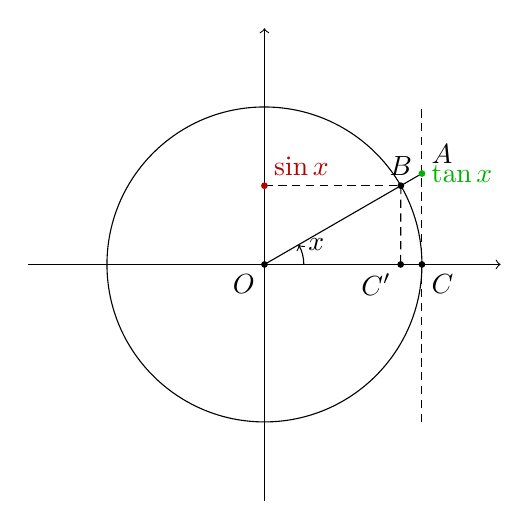
\begin{tikzpicture}
        \draw[black] (0, -0) circle (2);
        \draw[->] (-3, 0) -- (3, 0);
        \draw[->] (0, -3) -- (0, 3);
        \coordinate (A_pnt) at (30:2.31);
        \coordinate (B_pnt) at (30:2);
        \coordinate (C_p_pnt) at (1.73, 0);
        \coordinate (C_pnt) at (2, 0);
        \draw (0, 0) -- (A_pnt);
        \draw[densely dashed] (2, -2) -- (2, 2);
        \draw[densely dashed] (0, 1) -- (B_pnt);
        \filldraw[green!70!black] (A_pnt) circle(1pt) node[anchor=west]{$\tan x$};
        \filldraw[red!70!black] (0, 1) circle(1pt) node[anchor=south west]{$\sin x$};
        \draw[densely dashed] (B_pnt) -- (C_p_pnt);
        \filldraw[black] (0, 0) circle(1pt) node[anchor = north east]{$O$};
        \filldraw[black] (A_pnt) node[anchor = south west]{$A$};
        \filldraw[black] (B_pnt) circle(1pt) node[anchor = south]{$B$};
        \filldraw[black] (C_pnt) circle(1pt) node[anchor = north west]{$C$};
        \filldraw[black] (C_p_pnt) circle(1pt) node[anchor = north east]{$C'$};
        \draw[->] (0.5,0) arc (0:30:0.5) node[anchor=west]{$x$};
    \end{tikzpicture} \\
    & AC = \tan x, BC' = \sin x, \text{ дуга } \breve{BC} = x \cdot OC  \\
    & \text{Пусть $S_{BOC}, S_{AOC}$ - 
        площади соответствующих треугольников,
        $S_{\breve{BOC}}$ - площаль сектора, тогда} \\
    & S_{BOC} < S_{\breve{BOC}} < S_{AOC} \\
    & \frac{BC' OC}{2} < \frac{x OC^2}{2} < \frac{AC OC}{2} \\
    & \sin x < x < \tan x \\
    & \frac{\sin x}{x} < 1 < \frac{\sin x}{x \cos x} \\
    & \cos x < \frac{\sin x}{x} < 1 \\
    & \text{При } x \in \left(-\frac{\pi}{2}; 0\right) \text{ воспользуемся нечётностью синуса и чётностью косинуса:}\\
    & \frac{\sin x}{x} = \frac{\sin(-x)}{-x} \in (\cos(x); 1) \\
    & \text{Тогда } \forall x \in \dot{U}_{\frac{\pi}{2}}(0): \cos x < \frac{\sin x}{x} < 1 \\
    & \text{Распишем предел по определению сходимости по Коши:} 
        \forall \veps > 0 \, 
        \exists \delta(\veps) > 0 \, 
        \forall x \in \dot{U}_{\delta(\veps)}(0): 
        \left| \frac{\sin x}{x} - 1 \right| < \veps \\
    & \text{Будем выбирать только значения $\delta(\veps) \le \frac{\pi}{2}$, тогда} \\
    & \left| \frac{\sin x}{x} - 1 \right| < \veps
        \impliedby 1 - \frac{\sin x}{x} < \veps
        \impliedby 1 - \cos x < \veps
        \impliedby 1 - \cos^2 x < \veps
        \impliedby \sin^2 x < \veps \\
    &   \impliedby \sin x < \veps
        \impliedby x < \veps \\
    & \text{Показали, что если } 
        \forall \veps > 0: 
        \delta(\veps) := \min\left(\veps; \frac{\pi}{2}\right) 
        \text{, то определение предела по Коши выполняется}\\
\end{split}
}
}

\mcdfn{Второй замечательный предел}
{
    \[ \lim_{x \to +\infty} \left(1 + \frac{1}{x}\right)^x = e \]

\mcprf{
\begin{split}
    & \text{1. По определению числа Эйлера: } \lim_{n \to +\infty} \left(1 + \frac{1}{n}\right)^{n} = e \\
    & \text{По арифметике предела ч.п.: } \\
    & \lim_{n \to +\infty} \left(1 + \frac{1}{n + 1}\right)^{n} = e \\
    & \lim_{n \to +\infty} \left(1 + \frac{1}{n}\right)^{n + 1} = e \\
    & \text{По определению предела ч.п. это означает:} \\
    & \forall \veps > 0 \,
        \exists N_1(\veps) \in \Nset \, 
        \forall n > N_1(\veps): 
        \left| \left(1 + \frac{1}{n + 1}\right)^{n} - e \right| < \veps \\
    & \text{Последнее выражение равносильно: } e - \veps < \left(1 + \frac{1}{n + 1}\right)^{n} < e + \veps \\
    & \text{Аналогично } \\
    & \forall \veps > 0 \,
        \exists N_2(\veps) \in \Nset \, 
        \forall n > N_2(\veps): 
        e - \veps < \left(1 + \frac{1}{n}\right)^{n + 1} < e + \veps \\
    & \text{2. Хотим доказать: } \lim_{x \to +\infty} \left(1 + \frac{1}{x}\right)^x = e \\
    & \text{Распишем определение предела функции по Коши при $x \to +\infty$:} \\
    & \forall \veps > 0 \,
        \exists \delta = \delta(\veps) > 0 \,
        \forall x \in (\delta; +\infty):
        \left| \left(1 + \frac{1}{x}\right)^{x} - e \right| < \veps \\
    & \text{Будем рассматривать только $\delta \ge 1$, тогда:} \\
    & \forall x \in (\delta; +\infty) \,
        \exists n \in \Nset: n < x \le n + 1 \\
    & \text{Тогда } \left(1 + \frac{1}{n + 1}\right)^{n} < \left(1 + \frac{1}{x}\right)^{x} < \left(1 + \frac{1}{n}\right)^{n + 1} \\
    & \text{Положим } \delta(\veps) := \max\{N_1(\veps), N_2(\veps)\} + 1 \\
    & \text{Тогда для каждого рассматриваемого x: } n \ge x - 1 > \delta - 1 \ge \max\{N_1(\veps), N_2(\veps)\} \\
    & \text{То есть } n > N_1(\veps) \wedge n > N_2(\veps) \\
    & \text{Тогда } 
        e - \veps < \left(1 + \frac{1}{n + 1}\right)^{n} < \left(1 + \frac{1}{x}\right)^{x} < \left(1 + \frac{1}{n}\right)^{n + 1} < e + \veps
        \implies \\
    & \implies e - \veps < \left(1 + \frac{1}{x}\right)^{x} < e + \veps \\
    & \text{Таким образом, показали, что верно определение предела функции по Коши: } \\
    & \forall \veps > 0 \,
        \exists \delta = \max\{N_1(\veps), N_2(\veps)\} + 1 > 0 \,
        \forall x \in (\delta; +\infty):
        e - \veps < \left(1 + \frac{1}{x}\right)^{x} < e + \veps \\
\end{split}
}
}

\subsection{Теорема о пределе сложной функции}

\mcthm{Теорема о пределе сложной функции}
{
$$
\left. \begin{tabular}{l}
    $ \lim_{x\to x_0} f(x) = y_0 $ \\
    $ \lim_{y\to y_0} g(y) = g(y_0) $
\end{tabular} \right\}
\begin{tabular}{l}
    $ \implies \lim_{x \to x_0} g(f(x)) = g(y_0) $
\end{tabular}
$$
\begin{mcproof}
\begin{equation*}
\begin{split}
& \text{Распишем, что дано, по определению:} \\
& \forall \veps > 0 \, \exists \delta_1(\veps) \, \forall x \in \dot{U}_{\delta_1(\veps)}(x_0): | f(x) - y_0 | < \veps \, (1) \\
& \forall \lambda > 0 \, \exists \delta_2(\lambda) \, \forall y \in \dot{U}_{\delta_2(\lambda)}(y_0): | g(y) - g(y_0) | < \lambda \, (2) \\
& \text{Распишем, что хотим доказать:} \\
& \forall \eta > 0 \, \exists \delta_3 = \delta(\eta) \forall x \in \dot{U}_{\delta_3(\eta)}(x_0): | g(f(x)) - g(y_0) | < \eta \\
& \text{Положим } \delta_3(\eta) = \delta_1(\delta_2(\eta))\text{, тогда}: \\
& x \in \dot{U}_{\delta_3(\eta)}(x_0) \iff x \in \dot{U}_{\delta_1(\delta_2(\eta))}(x_0) \implies \text{ по (1) } | f(x) - y_0 | < \delta_2(\eta) \\
& | f(x) - y_0 | < \delta_2(\eta) \iff f(x) \in U_{\delta_2(\eta)}(y_0) \\
& \text{По (2) знаем, что если } f(x) \in \dot{U}_{\delta_2(\eta)}(y_0) \text{, то } | g(f(x)) - g(y_0) | < \eta \\
& \text{Если } f(x) = y_0 \text{, то } | g(f(x)) - g(y_0) | = 0 < \eta \\
& \text{Иначе, если } f(x) \ne y_0 \iff f(x) \in \dot{U}_{\delta_2(\eta)}(y_0) \text{, то } | g(f(x)) - g(y_0) | = 0 < \eta \\
& \text{Получили: } \forall \eta > 0 \, \exists \delta_3 = \delta_1(\delta_2(\eta)) \, \forall x \in \dot{U}_{\delta_3(\eta)}(x_0): | g(f(x)) - g(y_0) | < \eta \\
\end{split}
\end{equation*}
\end{mcproof}
}

%
% if lim != g(y_0), then lets take: f(x) === 0, g(y) = y == 0; f(x) -> 0 = y_0 when x -> 0; g(y) -> 0 = A when y -> y_0; g(f(x)) === 1 -> 1 = A when x -> x_0
%


\section{O - символика}

\mcdfn{O - символика}
{
\begin{tabular}{rl}
    o-малое:   & $\bullet $ $f(x) = \overline{o}(g(x)) $ при $ x \to x_0 \in \ExtRset $, 
                    если $ \frac{f(x)}{g(x)} $ - б.м. при $ x \to x_0 $ \\
    O-большое: & $\bullet $ $f(x) = \underline{O}(g(x)) $ при $ x \to x_0 \in \ExtRset $, 
                    если $ \frac{f(x)}{g(x)} $ - ограниченная при $ x \to x_0 $ \\
\end{tabular}
}

\section{Непрерывность функции}

\subsection{Непрерывность функции в точке}

\mcdfn{Непрерывность функции в точке}
{
    Функция называется непрерывной в точке $x_0$, если \[\lim_{x \to x_0} f(x) = f(x_0)\]
}

\mcclarf{}
{
    Если $x_0$ - граница области определения, то рассматривается односторонний предел
}

\subsection{Свойства непрерывных функций}

\nt{
    Свойства непрерывных функций:

\begin{tabular}{rl}
    & $\bullet$ Сумма, произведение и частное непрерывных функций - непрерывные функции \\
    & (по арифметике пределов функции) \\
    & $\bullet$ Композиция непрерывных функций - непрерывная функция \\
    & (по теореме о пределе сложной функции) \\
    & \begin{minipage}[t]{\textwidth}
    $$
    \left. \begin{tabular}{l}
        $ \lim_{x \to x_0} g(x) = g(x_0) = y_0 $ \\
        $ \lim_{y \to y_0} f(y) = f(y_0) $ \\
    \end{tabular} \right\}
    \begin{tabular}{l}
        $ \implies \lim_{x \to x_0} f(g(x)) = f(g(x_0)) $
    \end{tabular}
    $$
    \end{minipage} \\
\end{tabular}
}

\subsection{Правило замены переменных в пределе сложной функции}

\mcclm{Правило замены переменных в пределе}{}
{
    Пусть дана сложная функция $ f(g(x)) $, тогда, если для некоторой точки 
    $ x_0:  \lim_{x \to x_0} g(x) = g(x_0) = y_0 $ и $ \lim_{y \to y_0} f(y) = A \in \Rset $, то
    $ \lim_{x \to x_0} f(g(x)) = f(g(x_0)) $
}

\mcex{Пример использования правила замены переменной в пределе}
{
\[\begin{split}
    & \text{Пусть надо найти } \lim_{x \to 0} \frac{\sin(\pi x)}{x} \\
    & \text{Преобразуем выражение:} \frac{\sin(\pi x)}{x} = \frac{\sin(\pi x)}{\pi x} \cdot \pi \\
    & \text{В данном случае в обозначения из утверждения выше:} \\
    & f(y) = \frac{\sin(y)}{y} \\ 
    & g(x) = \pi x \\
    & g(x) \text{ непрерывна в точке } x_0 = 0, y_0 = g(x_0) = 0, \text{ и при этом } \lim_{y \to y_0} f(y) = 1 = A \\
    & \text{Тогда по правилу замены переменной в пределе:} \\
    & \lim_{x \to 0} \frac{\sin(\pi x)}{\pi x} \cdot \pi = \lim_{x \to 0} A \cdot \pi = \lim_{x \to 0} 1 \cdot \pi = \pi \\
\end{split}\]
}

\subsection{Непрерывность функции на множестве}

\mcdfn{Непрерывность функции на множестве}
{
    Функция называется непрерывной на множестве $E$, если она непрерывна в каждой точке множества $E$

    /* Когда говорят, что функция непрерывна, имеют ввиду, что она непрерывна на $D_f$ */
}

\nt{
    В частность, функция непрерывна на отрезке $[a;b]$, если она непрерывна в каждой точке отрезка $[a;b]$

    При этом, в точках $a$ и $b$ рассматриваются односторонние пределы
}

\subsection{Теорема 1 о функции, непрерывной на отрезке}

\mcthm{Теорема о функции, непрерывной на отрезке (иногда называют теоремой Вейерштрасса)}
{
    Функция, непрерывная на отрезке, ограничена на этом отрезке и достигает наибольшее и наименьшее значения на этом отрезке

    Докажем, что функция ограничена сверху и достигает наибольшее значение. Для второго случая доказательство проводится аналогично

\mcprf{
\begin{split}
    & \text{1. } E_f - \text{ мно-во значений } f(x) \text{ на } [a; b] \\
    & \text{Обозначим } M = \sup E_f = \sup_{x \in [a; b]} f(x) \in \ExtRset \\
    & \text{Построим некоторую строго возрастающую ч.п. } a_n \underset{n \to +\infty}{\to} M  \\
    & \text{2. Докажем, что } \forall n \in \mathbb{N} \, \exists x_n \in [a; b]: a_n < f(x_n) \\
    & \text{Предположим от противного, то есть } \exists n_0 \, \forall x \in [a; b]: a_{n_0} \ge f(x) \\
    & \text{Тогда } a_{n_0} \text{ - верхняя грань множества $E_f$} \\
    & \text{Однако, т.к. $a_n$ - возрастающая ч.п. и $ \lim_{n \to +\infty} a_n = a $ , то } \forall n \in \mathbb{N}: a_n < M \\
    & \text{В частности, } a_{n_0} < M \text{, т.е. $a_{n_0}$ - верхняя грань, которая меньше точной верхней грани } \implies \\
    & \implies \circled{$\mathbb{W}$} \implies \forall n \in \mathbb{N} \, \exists x_n \in [a; b]: a_n < f(x_n) \\
    & \text{3. По построению } \forall x \in [a; b]: f(x) \le M \\
    & \text{Тогда } \forall n \in \mathbb{N} \, \exists x_n \in [a; b]: a_n < f(x_n) \le M \\
    & \text{Следовательно, по теореме о зажатой последовательности } \lim_{n \to +\infty} f(x_n) = M \\
    & \text{4. Докажем, что } M = f(x_0) \\
    & \text{Т.к. $x_n$ - ограниченная ч.п., то по теореме Больцано-Вейерштрасса из неё можно выделить} \\
    & \text{сходящуюся подпоследовательность } \NumSeq{x_{n_k}} \text{ такую, что } x_{n_k} \underset{k \to +\infty}{\to} x_0 \in [a; b] \\
    & \text{Т.к. $f$ непрерывна в на отрезке, то она непрерывна в $x_0$, следовательно} \\
    & \lim_{k \to +\infty} f(x_{n_k}) = f(x_0) \\
    & \left(\lim_{n \to +\infty} f(x_n) = M\right) \wedge \left(\lim_{k \to +\infty} f(x_{n_k}) = f(x_0)\right) \implies M = f(x_0) < \infty \\
    & \text{Таким образом, на отрезке $ [a;b] $ функция $f$ ограничена сверху числом $M = f(x_0)$} \\
\end{split}
}
}

\subsection{Теорема 2 о функции, непрерывной на отрезке}

\mcthm{Теорема (2) о функции, непрерывной на отрезке}
{
    Функция, непрерывная на отрезке $[a;b]$, принимает все промежуточные значения

    Пусть $f(x)$ непрерывна на $[a;b], f(x_1) = A, f(x_2) = B, x_1 < x_2, $ БОО $ A < B $, тогда

    $ \forall c \in (A; B) \, \exists x_0 \in (x_1; x_2): f(x_0) = c $

\mcprf{
\begin{split}
    & \text{1. Построим последовательность вложенных отрезков:} \\
    & \text{/* Если Вам так будет удобнее, то докажем существование $x_0$ бинпоиском по ответу */} \\
    & [a_1; b_1] := [x_1; x_2] \\
    & x_3 := \frac{a_1 + b_1}{2} \text{, рассмотрим $f(x_3)$} \\
    & 1) f(x_3) = c \implies q.e.d. \\
    & 2) f(x_3) < c \implies [a_2; b_2] := [x_3; b_1] \\
    & 3) f(x_3) > c \implies [a_2; b_2] := [a_1; x_3] \\
    & \text{Применяя это правило, продолжим строить последовательность отрезков} \\
    & \text{Если ни на какой итерации не произойдёт случай $1)$, то получим счётно бесконечную} \\
    & \text{последовательность отрезков} \NumSeq{[a_n; b_n]}_{n \in \mathbb{N}} \\
    & \text{По построению ч.п. } \NumSeq{a_n} \text{ неубывает и ограничена сверху } b \implies \exists \lim_{n \to +\infty} a_n \le b \\
    & \text{По построению ч.п. } \NumSeq{b_n} \text{ невозрастает и ограничена снизу } a \implies \exists \lim_{n \to +\infty} b_n \ge a \\
    & b_n - a_n = \frac{b - a}{2^{n - 1}} \to_{n \to +\infty} 0 \implies \lim_{n \to +\infty} a_n = \lim_{n \to +\infty} b_n = x_0 \\
    & x_0 \in [a; b] \implies f(x) \text{ непрерывна в } x_0 \implies \lim_{x \to x_0} f(x) = f(x_0) \implies \\
    & \implies \text{по определению по Гейне } \lim_{n \to +\infty} f(a_n) = \lim_{n \to +\infty} f(b_n) = f(x_0) \\
    & \text{По построению } f(a_n) < c \wedge f(b_n) > c \implies c \le f(x_0) \le c \implies f(x_0) = c \\
\end{split}
}
}

\subsubsection{Следствие 1}

\mccorollar{Следствие}{
    $ f(x) $ непрерывна на $ [a;b] \implies E_f = [\inf E_f; \sup E_f] $
}

\subsubsection{Следствие 2}

\mccorollar{Следствие}{
    $ f(x) = x^2 $ непрерывна на $ D_f = [0; 2] \implies (E_f = [0; 4] \wedge \exists x_0 \in \Rset: x_0^2 = 2) $

    То есть доказано существование числа $\sqrt{2}$
}

\subsubsection{Следствие 3}

\mccorollar{Следствие}{
    $ f(x) \text{ непрерывна на } [a; b] \wedge f(a) < 0 \wedge f(b) > 0 \implies \exists c \in (a; b): f(c) = 0 $ 
}

\subsection{Определение монотонности функции}

\mcdfn{Определение монотонности функции}{
\begin{tabular}{rl}
    & $\bullet$ $f(x)$ называется строго возрастающей на $E \subseteq \Rset$, если 
        $\forall x_1, x_2 \in E: x_1 < x_2 \implies f(x_1) < f(x_2) $ \\
    & $\bullet$ $f(x)$ называется неубывающей на $E \subseteq \Rset$, если 
        $\forall x_1, x_2 \in E: x_1 < x_2 \implies f(x_1) \le f(x_2) $ \\
    & $\bullet$ $f(x)$ называется строго убывающей на $E \subseteq \Rset$, если 
        $\forall x_1, x_2 \in E: x_1 < x_2 \implies f(x_1) > f(x_2) $ \\
    & $\bullet$ $f(x)$ называется невозрастающей на $E \subseteq \Rset$, если 
        $\forall x_1, x_2 \in E: x_1 < x_2 \implies f(x_1) \ge f(x_2) $ \\
\end{tabular}
}

\subsection{Достаточное условие обратимости}

\mcdfn{Достаточное условие обратимости}{
    Если функция $f(x)$ строго монотонна на $X$, то $f(x)$ обратима на $X$
\mcprf{
\begin{split}
    & \text{Предположим от противного, что $f(x)$ не инъективна, то есть} \\
    & \exists x_1, x_2 \in X: x_1 \ne x_2 \wedge f(x_1) = f(x_2) \\
    & x_1 \ne x_2 \implies \min(x_1, x_2) < \max(x_1, x_2) \implies \circled{$\mathbb{W}$} \text{ с определением строгой монотонности} \\
\end{split}
}
}

\subsection{Критерий обратимости функции}

\mcdfn{Критерий обратимости функции}
{
    Пусть функция $f(x)$ непрерывна на $[a;b]$. Тогда $f(x)$ обратима $\iff f(x)$ строго монотонна
\mcprf{
\begin{split}
    & "\impliedby" \text{Смотри достаточное условие обратимости} \\
    & "\implies" \\
    & \text{Докажем для случая, когда $f(x)$ строго монотонно возрастает, для убывания аналогично} \\
    & \text{Предположим от противного, тогда БОО} \\
    & \exists x_1 < x_2 < x_3 \in [a; b]: \, f(x_1) < f(x_2) \ge f(x_3)  \\
    & \text{Если } f(x_2) = f(x_3) \text{, то $f$ не инъективна } \implies \text{ $f$ не обратима } \implies \circled{$\mathbb{W}$} \\
    & \text{Иначе, положим } c := \frac{\max(f(x_1), f(x_3)) + f(x_2)}{2} \implies f(x_1) < c < f(x_2) \wedge f(x_3) < c < f(x_2)  \\
    & f \text{ непрерывна на } [a; b] \implies f \text{ непрерывна на } [x_1; x_2] \text{ и } [x_2; x_3] \\
    & f \text{ непрерывна на } [x_1; x_2] \implies \exists x_0' \in (x_1; x_2): f(x_0') = c \\
    & f \text{ непрерывна на } [x_2; x_3] \implies \exists x_0'' \in (x_2; x_3): f(x_0'') = c \\
    & \text{Получили: } \exists x_0' < x_0'' \in [a; b]: f(x_0') = f(x_0'') \implies \text{ $f$ не инъективна } \implies \text{ $f$ не обратима } \implies \circled{$\mathbb{W}$} \\ \\
\end{split}
}
}

\subsection{Свойства обратимой функции}

\mcthm{}{
    Если функция $f(x)$ непрерывна и строго монотонна на $[a;b]$, то функция $f^{-1}(y):$

\begin{tabular}{rl}
& $\bullet$ 1) определена на $ E_f = [\min(f(a), f(b)); \max(f(a), f(b))] $ \\
& $\bullet$ 2) мотонотонна (и имеет ту же монотонность) на $ E_f $ \\
& $\bullet$ 3) непрерывна на $ E_f $ \\
\end{tabular}

\mcprf{
\begin{split}
    & \text{1. Доказано по критерию обратимости функции} \\
    & \text{2. БОО $f$ возрастает на $[a; b]$} \\
    & \text{Предположим от противного} \\
    & f^{-1}(y) \text{ не возрастает на } [a; b] \implies \exists y_1 < y_2 \in [f(a); f(b)]: f^{-1}(y_1) \ge f^{-1}(y_2) \\
    & \text{По определению обратной функции } f^{-1}(y_1), f^{-1}(y_2) \in [a; b] \text{, обозначим } x_1 = f^{-1}(y_1), x_2 = f^{-1}(y_2) \\
    & x_1 \ge x_2 \implies f(x_1) \ge f(x_2) \text{. При этом, } f(x_1) = y_1 \wedge f(x_2) = y_2 \\
    & x_1 \ge x_2 \implies y_1 \ge y_2 \implies \circled{$\mathbb{W}$} \\
    & \text{3. Докажем непрерывность по определению} \\
    & \text{Дано: } x = f^{-1}(y) \text{ - определённая монотонная на $[a; b]$ функция} \\
    & \text{Докажем, что $f^{-1}$ непрерывна в любой точке } y_0 \in (f(a); f(b)) \\
    & \text{Для } y_0 \in \{ f(a), f(b) \} \text{ доказательство аналогично (нужно рассмотреть односторонние пределы)} \\
    & \text{По определению непрерывности в точке } 
        \forall \veps > 0 \,
        \exists \delta > 0 \,
        \forall y \in \dot{U}_\delta(y_0): 
        | f^{-1}(y) - f^{-1}(y_0) | < \veps \\
    & \text{Обозначим } f^{-1}(y_0) = x_0 \\
    & \text{БОО докажем для таких $\veps$, что } 
        U_\veps(x_0) \subset (a; b) \text{. Для } \emph{б\'{o}льших } \veps \text{ неравество также будет выполняться} \\
    & a < x_0 - \veps < x_0 + \veps < b \\
    & \text{Обозначим } y_1 = f(x_0 - \veps), y_2 = f(x_0 + \veps), \text{ тогда } y_1 < y_0 < y_2 \\
    & \text{Положим } \delta := \min(y_2 - y_0, y_0 - y_1) \text{, тогда } U_\delta(y_0) \in (y_1; y_2) \\
    & \text{Докажем, что при выбранном $\delta$ выполняется неравенство под знаками кванторов:} \\
    & y \in U_\delta(y_0) 
        \implies y \in (y_1; y_2) 
        \implies f^{-1}(y_1) < f^{-1}(y) < f^{-1}(y_2) 
        \implies x_0 - \veps < f^{-1}(y) < x_0 + \veps \implies \\
    &   \implies | f^{-1}(y) - x_0 | < \veps
        \implies \text{ неравенство под кванторами верно и определение выполняется} \\
\end{split}
}
}

\subsubsection{Следствие 1}

\mccorollar{Следствие (без доказательства)}{
    Если функция $f(x)$ непрерывна и строго монотонна на $(a; b), \, a, b \in \ExtRset$, то функция $f^{-1}(y):$

\begin{tabular}{rl}
    & $\bullet$ 1) определена на $ (m; M) $, где $ m = \min(f(a), f(b)), M = \max(f(a), f(b)) $ \\
    & $\bullet$ 2) мотонотонна (и имеет ту же монотонность) $ [m; M] $ \\
    & $\bullet$ 3) непрерывна на $ (m; M) $ \\
\end{tabular}

    Идея доказательства: рассмотреть $[c;d] \subset (a; b)$, для него верна теорема выше, а далее перейти к пределу при границах, стремящихся к $a$ и $b$
}

\subsubsection{Следствие 2}

\mccorollar{}{
    Т.к. $f(x) = x^n$ непрерывна и строго монотонно возрастает на $D_f = n \,\, \vdots \,\, 2 \, ? \, [0; +\infty) \, : \, \Rset$, то

    $g(x) = \sqrt[n]{x} $ непрерывна и строго монотонно возрастает на $D_g = E_f = n \,\, \vdots \,\, 2 \, ? \, [0; +\infty) \, : \, \Rset$
}

\subsection{Обратные тригонометрические функции}

\mcdfn{Обратные тригонометрические функции}{
    $ y = \sin x $ непрерывна и возрастает на $ D_f = [-\frac{\pi}{2}; \frac{\pi}{2}] \implies $

    $ \implies \exists \arcsin := \sin^{-1}: y = \arcsin x $ непрерывна и возрастает на $ E_f = [-\frac{\pi}{2}; \frac{\pi}{2}] $, область значений - $D_f = [-1; 1]$

    Аналогично

    \begin{tabular}{rl}
        & $\bullet$ $ y = \arccos x $ непрерывна и убывает на $E_f = [0; \pi] $, область значений - $D_f = [-1; 1]$ \\
        & $\bullet$ $ y = \arctan x $ непрерывна и возрастает на $E_f = (-\frac{\pi}{2}; \frac{\pi}{2})$, область значений - $D_f = \Rset$ \\
        & $\bullet$ $ y = \text{arcctg} \, x $ непрерывна и убывает на $E_f = (0; \pi)$, область значений - $D_f = \Rset$ \\
    \end{tabular}
}

\subsection{Показательная функция}

\mcdfn{Показательная функция}{
    (теорема без доказательства) функция $y = a^x, a > 0$

\begin{tabular}{rl}
    & $\bullet$ 1) определена на $ D_f = \Rset, E_f = (0; +\infty) $ \\
    & $\bullet$ 2) возрастает при $ a > 1 $ и убывает при $ 0 < a < 1 $ \\
    & $\bullet$ 3) непрерывна на $ \Rset $ \\
    & $\bullet$ 4) $a^{x} \cdot a^{y} = a^{x + y} $ \\
    & \,\,\,\, /* Следствие: $\phi(x) = a^x$ является изоморфизмом между $(\Rset, +)$ и $(\Rset_+, *)$ */ \\
    & \,\,\,\, $(a^x)^y = a^{xy} $\\
\end{tabular}
}

\subsection{Логарифмическая функция}

\mcdfn{Логарифмическая функция}{
    Функция, обратная к $y = a^x, a \in (0; 1) \cup (1; +\infty)$ обозначается $ y = \log_{a}x$

\begin{tabular}{rl}
    & $\bullet$ 1) определена на $ D_f = (0; +\infty), E_f = \Rset $ \\
    & $\bullet$ 2) возрастает при $ a > 1 $ и убывает при $ 0 < a < 1 $ \\
    & $\bullet$ 3) непрерывна на $ (0; +\infty) $ \\
    & $\bullet$ 4) $ \log_a{x} + \log_a{y} = \log_a xy $ \\
    & \,\,\,\, /* Следствие: $\psi(x) = \log_a{x}$ является изоморфизмом между $(\Rset_+, *)$ и $(\Rset, +)$ */ \\
    & \,\,\,\, $ \log_a{x^\alpha} = \alpha \log_a{x} $\\
\end{tabular}
}

\subsection{Следствия из 2 замечательного предела}

\mccorollar{Следствия из 2 замечательного предела}{
    $ \lim_{x \to 0} (1 + x)^\frac{1}{x} = e $

    $ \lim_{x \to 0} \frac{\ln(x + 1)}{x} = 1 $

\mcprf{
\begin{split}
    & \frac{\ln(x + 1)}{x} = \frac{1}{x} \ln(x + 1) = \ln(x + 1)^\frac{1}{x} \\
    & \text{Функция $\ln x$ непрерывна, тогда по теореме о пределе сложной функции} \\
    & \lim_{x \to 0} \frac{\ln(x + 1)}{x} = \lim_{x \to 0} \ln(x + 1)^\frac{1}{x} = 1 \\
\end{split}
}

    $ \lim_{x \to 0} \frac{e^x - 1}{x} = 1 $

\mcprf{
\begin{split}
    & t = e^x - 1 \implies x = \ln(t + 1) \\
    & x \to 0 \implies t \to \infty \\
    & \lim_{x \to 0} \frac{e^x - 1}{x} = \lim_{t \to 0} \frac{t}{\ln(t + 1)} = 1 \\
\end{split}
}
}

\subsection{Показательная функция с вещественным показателем}

\mccorollar{Показательная функция с вещественным показателем}{
    $ y = x^\alpha, \alpha \in \Rset, D_f = (0; +\infty) $

    $ y = e^{\alpha \ln x} $

    $ \ln x $ непрерывна и возрастает на $(0; +\infty)$

    $ \alpha \ln x $ непрерывна и возрастает при $\alpha > 0 $ и убывает при $\alpha < 0$

    $ e^{\alpha \ln x} $ непрерывна и возрастает при $\alpha > 0 $ и убывает при $\alpha < 0$
}

\subsubsection{Следствие}

\mccorollar{}{
    $ \lim_{x \to +\infty} a(x) = a \wedge 
        \lim_{x \to +\infty} b(x) = b \implies
        \lim_{x \to +\infty} a(x)^{b(x)} = \lim_{x \to +\infty} e^{b(x) \ln a(x)} = e^{b \ln a} = a^b $

    Для ч.п. $ \NumSeq{a_n} $ и $ \NumSeq{b_n} $ построим кусочно-линейные функции $a(x)$ и $b(x)$, такие что $ \forall n \in \mathbb{N}: a(n) = a_n \wedge b(n) = b_n $

    Тогда $ \lim_{n \to +\infty} a_n = a \wedge \lim_{n \to +\infty} b_n = b \implies \lim_{n \to +\infty} a_n^{b_n} = a^b $ 
}

\section{Производная функции}

\subsection{Определение производной}

\mcdfn{Определение производной}{
    Производная функции $ f $ в точке $x_0$ - это предел

$$
\lim_{\Delta x \to 0} \frac{\Delta f}{\Delta x} = \lim_{x \to x_0} \frac{f(x) - f(x_0)}{x - x_0} = f'(x_0)
$$
}

\nt{
    $ \forall x \in \Rset: \, (\sin x)' = \cos x $

\mcprf{
\begin{split}
    & \lim_{x \to x_0} \frac{\sin x - \sin x_0}{x - x_0} = 
        \lim_{x \to x_0} \frac{2 \sin (\frac{x - x_0}{2}) \cos(\frac{x + x_0}{2})}{x - x_0} =
        \lim_{x \to x_0} \cos(\frac{x + x_0}{2}) = \cos x_0 \\
\end{split}
}
}

\nt{
    $ \forall x \in \Rset \, \forall n \in \mathbb{N}: \, (x^n)' = n x^{n - 1} $

\mcprf{
\begin{split}
    & \lim_{x \to x_0} \frac{x^n - {x_0}^n}{x - x_0} = 
        \lim_{x \to x_0} \frac{(x - x_0) \sum_{k = 0}^{n - 1} x^{n - 1 - k} {x_0}^{k}}{x - x_0} = 
        \lim_{x \to x_0} \sum_{k = 0}^{n - 1} x^{n - 1 - k} {x_0}^{k} = n x_0^{n - 1} \\
\end{split}
}
}


\nt{
    $ (a^x)' = a^x \ln a $

\mcprf{
\begin{split}
    & \lim_{x \to x_0} \frac{a^x - a^{x_0}}{x - x_0} = 
        a^{x_0} \lim_{x \to x_0} \frac{a^{x - x_0} - 1}{x - x_0} = 
        a^{x_0} \lim_{t \to 0} \frac{a^{t} - 1}{t} = \\
    & = a^{x_0} \lim_{t \to 0} \frac{e^{t \ln a} - 1}{t} =
        a^{x_0} \lim_{s \to 0} \frac{e^{s} - 1}{s} \cdot \ln a = a^{x_0} \ln a \\
\end{split}
}
}

\nt{$ (e^x)' = e^x $}

\subsection{Правила подсчёта производных}

\mcclm{Правила подсчёта производных}{}{
    Если $ \exists f'(x), \exists g'(x), \alpha \in \Rset, \beta \in \Rset $, то

	\begin{tabular}{rl}
		& $\bullet$ $ (\alpha f(x) + \beta g(x))' = \alpha f'(x) + \beta g'(x) $ \\
		& $\bullet$ $ (f(x) \cdot g(x))' = f'(x) \cdot g(x) + f(x) \cdot g'(x) $ \\
        & $\bullet$ $ g(x) \ne 0 \implies \left(\frac{f(x)}{g(x)}\right)' = \frac{f'(x) g(x) - f(x) g'(x)}{g^2(x)} $ % proof at lecture 11, 1:10:30 %
	\end{tabular}
}

\subsection{Определения дифференцируемости функции}

\mcdfn{Дифференцируемость функции в точке}{
    Функция $f(x)$ называется дифференцируемой в точке $x_0$, если
\[ \exists A(x_0) \in \Rset: \, f(x) = f(x_0) + A(x_0) \cdot (x - x_0) + \SmO[x - x_0] \]

    Где $ A(x_0) $ - некоторая величина, не зависящая от $ x $ (т.е. для каждой точки $ x_0 $ это некоторое число)
}

\mcthm{Признак дифференцируемости функции в точке}{
    Функция $f(x)$ дифференцируема в точке $x_0 \iff \exists f'(x_0) \in \Rset $
\mcprf{
\begin{split}
    & "\implies" \\
    & \text{По определению дифференцируемости в точке} \\
    & \exists A(x_0) \in \Rset: \, f(x) = f(x_0) + A(x_0) \cdot (x - x_0) + \SmO[x - x_0] 
        \implies \frac{f(x) - f(x_0)}{x - x_0} = A(x_0) + \SmO[1] \implies \\
    & \lim_{x \to x_0} \frac{f(x) - f(x_0)}{x - x_0} = A(x_0) \in \Rset \implies
        \exists f'(x_0) = A(x_0) \in \Rset \\
    & "\impliedby" \\
    & \text{По определению производной:} \\
    & \exists \lim_{x \to x_0} \frac{f(x) - f(x_0)}{x - x_0} = f'(x_0) \in \Rset
        \implies \frac{f(x) - f(x_0)}{x - x_0} = f'(x_0) + \SmO[1] \implies \\
    & \implies f(x) - f(x_0) = f'(x_0) \cdot (x - x_0) + \SmO[x - x_0] \\
    & \implies f(x) = f(x_0) + A(x_0) \cdot (x - x_0) + \SmO[x - x_0], A(x_0) = f'(x_0) \in \Rset \\
\end{split}
}
}

\subsection{Определение дифференциала}

\mcdfn{Определение дифференциала}{
    Дифференциал функции $f(x)$ в точке $x_0$ - 
    это линейная функция $ d f(x_0) = A(x_0) \cdot (x - x_0) $ такая, что
    $ f(x) = f(x_0) + d f(x_0) + \SmO[x - x_0] $

    Обозначив $x - x_0$ как $dx$ (фиксированное приращение), получим:

    $ d f(x_0) = f'(x_0) dx $
}

\subsection{Теорема о непрерывности функции, дифференцируемой в точке}

\mcthm{}{
    Дифференцируемая в точке $x_0$ функция непрерывна в ней
\mcprf{
\begin{split}
    & \text{По определению дифференцируемости в точке } x_0: \\
    & f(x) = f(x_0) + f'(x_0) \cdot (x - x_0) + \SmO[x - x_0] \\
    & \left. \begin{tabular}{l}
        $ f'(x_0) \in \Rset \implies \lim_{x \to x_0} f'(x_0) \cdot (x - x_0) = 0 $ \\
        $ \lim_{x \to x_0} \SmO[x - x_0] = 0 $
    \end{tabular} \right\}
    \begin{tabular}{l}
        $ \implies \lim_{x \to x_0} f(x) = x_0 $
    \end{tabular} \\
\end{split}
}
}

\subsection{Теорема о дифференцируемости сложной функции}

\mcthm{}{
    Если $g(x)$ дифференцируема в точке $ x_0 $ и функция $f(y)$ дифференцируема в точке $y_0 = g(x_0)$, то
    $f(g(x))$ дифференцируема в точке $ x_0 $ и $ (f(g(x)))' \vert_{x = x_0} = f'(g(x_0)) \cdot g'(x_0) $
\mcprf{
\begin{split}
    & g(x) = g(x_0) + g'(x_0) (x - x_0) + \SmO[x - x_0] \\
    & f(y) = f(y_0) + f'(y_0) (y - y_0) + \SmO[y - y_0] \implies \\
    & f(g(x)) = f(g(x_0)) + f'(g(x_0)) (g'(x_0) (x - x_0) + \SmO[x - x_0]) + \SmO[g'(x_0) (x - x_0) + \SmO[x - x_0]] \\
    & f(g(x)) = f(g(x_0)) + f'(g(x_0)) g'(x_0) (x - x_0) + f'(g(x_0)) \cdot \SmO[x - x_0] + \SmO[g'(x_0) (x - x_0) + \SmO[x - x_0]] = \\
    & = f(g(x_0)) + f'(g(x_0)) g'(x_0) (x - x_0) + \SmO[x - x_0]  + (x - x_0) \SmO[g'(x_0) + \SmO(1)] = \\
    & = f(g(x_0)) + f'(g(x_0)) g'(x_0) (x - x_0) + \SmO[x - x_0] \implies (f(g(x)))' \vert_{x = x_0} = f'(g(x_0)) \cdot g'(x_0) \\
\end{split}
}
}

\subsection{Теорема о производной обратной функции}

\mcthm{}{
    Если $f(x)$ непрерывна и обратима на $[a; b]$, $x_0 \in (a; b), \exists f'(x_0) \ne 0 $, тогда
    $ \exists (f^{-1}(y))'|_{y = f(x_0) = y_0} = \frac{1}{f'(x_0)} $

\mcprf{
\begin{split}
    & \lim_{y \to y_0} \frac{f'(y) - f'(y_0)}{y - y_0}
        = \vert \text{замена } y = f(x) \vert
        = \lim_{x \to x_0} \frac{f^{-1}(f(x)) - f^{-1}(f(x_0))}{f(x) - f(x_0)}
        = \lim_{x \to x_0} \frac{x - x_0}{f(x) - f(x_0)} = \frac{1}{f'(x_0)} \\
\end{split}
}
}

\subsection{Пример 1}

\mcex{}{
    Пример: $ f(x) = e^x, f'(x) = e^x, f^{-1}(y) = \ln y $

    $ (f^{-1}(y))'|_{y = y_0} = \frac{1}{f'(f^{-1}(y_0))} = \frac{1}{e^{f^{-1}(y_0)}} = \frac{1}{e^{\ln y_0}} = \frac{1}{y_0}  $
}

\subsection{Пример 2}

\mcex{}{
    Пример: $y = x^\alpha, \alpha \in \Rset, D_f = (0; +\infty)$

    $ y = e^{\alpha \ln x} \implies y' = e^{\alpha \ln x} (\alpha \ln x)' = e^{\alpha \ln x} \cdot \frac{\alpha}{x} = \alpha x^{\alpha - 1} $
}

\subsection{Определение локального минимума}

\mcdfn{Определение локального минимума (точка минимума)}{
    $ x_0 $ - точка локального минимума функции f(x), если 
    $ \exists \delta_0 > 0 \, \forall x \in U_{\delta_0}(x_0): f(x_0) \le f(x) $

    $ x_0 $ - точка строгого локального минимума функции f(x), если 
    $ \exists \delta_0 > 0 \, \forall x \in \dot{U}_{\delta_0}(x_0): f(x_0) < f(x) $
}

\subsection{Определение локального максимума}

\mcdfn{Определение локального максимума (точка максимума)}{
    $ x_0 $ - точка локального максимума функции f(x), если 
    $ \exists \delta_0 > 0 \, \forall x \in U_{\delta_0}(x_0): f(x_0) \ge f(x) $

    $ x_0 $ - точка строгого локального максимума функции f(x), если 
    $ \exists \delta_0 > 0 \, \forall x \in \dot{U}_{\delta_0}(x_0): f(x_0) > f(x) $
}

\subsection{Определение точки локального экстремума}

\mcdfn{Точка локального экстремума}{
    Точками локального экстремума называются точки минимума и точки максимума
}

\subsection{Необходимое условие локального экстремума (теорема Ферма)}

\mcthm{Необходимое условие локального экстремума (теорема Ферма)}{
    Если $x_0$ - точка локального экстремума, то $ \exists f'(x_0) \implies f'(x_0) = 0 $
\mcprf{
\begin{split}
    & \text{Пусть $\exists f'(x_0)$} \\
    & \text{Докажем для случая, когда $x_0$ - локальный минимум, для локального максимума } \\
    & \text{доказательство аналогично.} \\
    & \text{Предел при $ x \to x_0 $ существует $\implies$ существуют односторонние пределы и они совпадают с $f'(x_0)$ } \\
    & \text{В некоторой $ \delta $ окрестности } f(x_0) \le f(x) \\
    & \left. \begin{tabular}{l}
        $ x > x_0 \implies x - x_0 > 0 \implies \lim_{x \to x_0+} \frac{f(x) - f(x_0)}{x - x_0} \ge 0 $ \\
        $ x < x_0 \implies x - x_0 < 0 \implies \lim_{x \to x_0-} \frac{f(x) - f(x_0)}{x - x_0} \le 0 $ \\
    \end{tabular} \right\}
    \begin{tabular}{l}
        $ \implies f'(x_0) = \lim_{x \to x_0} \frac{f(x) - f(x_0)}{x - x_0} = 0 $
    \end{tabular} \\
\end{split}
}
}

\subsection{Определения касательной к графику функции}

\mcdfn{Касательная к графику функции}{
    Касательной к графику функции $f(x)$ называется прямая $ y = f'(x_0) (x - x_0) + f(x_0) $ 
}

\subsection{Теорема Ролля}

\mcthm{Теорема Ролля}{
    Если функция $ f(x) $ удовлетворяет условиям:

\begin{tabular}{rl}
    & $\bullet$ Непрерывна на $[a; b]$ \\
    & $\bullet$ Дифференцируема на $(a; b)$\\
    & $\bullet$ $f(a) = f(b)$\\
\end{tabular}

    То $ \exists \xi \in (a; b): f'(\xi) = 0 $
\mcprf{
\begin{split}
    & \text{1. Обозначим } M := \sup_{x \in [a; b]} f(x), m := \inf_{x \in [a; b]} f(x) \text{ достигаются, т.к. функция непрерывна на отрезке} \\
    & \text{2. Если } m = M \implies f(x) = const \implies \forall x \in (a; b): f'(x) = 0 \\
    & \text{3. Иначе, если $m < M$, тогда хотя бы одна из этих точек достигается в $ \xi \in (a; b)$ (т.к. $f(a) = f(b)$) } \\
    & \text{БОО } f(\xi) = M \implies \xi \text{ - точка loc max } \\
    & \text{$f$ дифференцируема на } (a; b) \implies \exists f'(\xi) \implies f'(\xi) = 0 \text{ (по теореме Ферма)} \\
\end{split}
}
}

\subsection{Теорема Лагранжа}

\mcthm{Теорема Лагранжа}{
    Если функция $ f(x) $ удовлетворяет условиям:

\begin{tabular}{rl}
    & $\bullet$ Непрерывна на $[a; b]$ \\
    & $\bullet$ Дифференцируема на $(a; b)$\\
\end{tabular}

    То $ \exists \xi \in (a; b): \frac{f(b) - f(a)}{b - a} = f'(\xi) $
\mcprf{
\begin{split}
    & \text{1. Рассмотрим } F(x) = f(x) - \frac{f(b) - f(a)}{b - a} x \text{, эта функция также, как и функция $f$, } \\
    & \text{непрерывна на $[a; b]$ и дифференцируема на $(a; b)$} \\
    & F(a) = F(b) 
        \implies \text{ для $F$ выполняются требования теоремы Ролля }
        \implies \exists \xi \in (a; b): F'(\xi) = 0 \implies \\
    & \implies \exists \xi \in (a; b): f'(\xi) - \frac{f(b) - f(a)}{b - a} = 0 
        \implies \exists \xi \in (a; b): \frac{f(b) - f(a)}{b - a} = f'(\xi) \\
\end{split}
}
}

\subsection{Теорема-следствие 1}

\mccorollar{Теорема-следствие 1}{
    Если функция $ f(x) $ удовлетворяет условиям:

\begin{tabular}{rl}
    & $\bullet$ Непрерывна на $[a; b]$ \\
    & $\bullet$ Дифференцируема на $(a; b)$\\
    & $\bullet$ $f'(x) = 0$ на $(a; b)$\\
\end{tabular}

    То $ f(x) = const $ на $ [a; b] $
\mcprf{
\begin{split}
    & \forall x_1, x_2 \in [a; b] f(x) \text{ удовлетворяет требованиям теоремы Лагранжа на } [x1_; x_2] \implies \\
    & \implies \exists \xi \in (x_1; x_1): f(x_2) - f(x_1) = f'(\xi) (x_2 - x_1) = 0 \cdot (x_2 - x_1) \\
    & \text{Получили: } \forall x_1, x_2 \in [a; b]: f(x_2) - f(x_1) = 0 \\
\end{split}
}
}

\subsection{Теорема-следствие 2}

\label{theorem_corollary_2:1}

\mccorollar{Теорема-следствие 2}{
    Если функции $ f(x) $ и $g(x)$ удовлетворяют условиям:

    \begin{tabular}{rl}
        & $\bullet$ Непрерывность на $[a; b] $\\
        & $\bullet$ Дифференцируемость на $(a; b) $\\
        & $\bullet$ $ \forall x \in (a; b): f'(x) = g'(x) $\\
    \end{tabular}

    То $ \forall x \in [a; b]: f(x) - g(x) = const $

\mcprf{
\begin{split}
    & \text{Рассмотрим } h(x) = f(x) - g(x) \\
    & h(x) \text{ удовлетворяет требованиям предыдущей теоремы-следствия 1} \implies \\
    & \implies \forall x \in [a; b]: f(x) - g(x) = const \\
\end{split}
}
}

\subsection{Теорема-следствие 3}

\mccorollar{Теорема-следствие 3}{
    Если $\phi(x)$ непрерывна на $ [a; b] $ и $ \phi'(x) $ определена везде на $ (a; b) $, 
        кроме, быть может, $x_0$, и $ \exists \lim_{x \to x_0} \phi'(x) = A \in \Rset $

    То $ \exists \phi'(x_0) = A $, т.е. у производной непрерывной функции нет точек устранимого разрыва
\mcprf{
\begin{split}
    & \text{По определению производной и по теореме Лагранжа:} \\
    & \phi'(x_0) 
        = \lim_{x \to x_0} \frac{\phi(x) - \phi(x_0)}{x - x_0} 
        = \lim_{x \to x_0} \phi'(\xi(x)), \xi(x) \in (x_0; x)
        \text{, т.к. на } (x_0; x) \\
    & \phi(x) \text{ удовлетворяет требованиям т. Лагранжа} \\
    & \lim_{x \to x_0} \xi(x) = x_0 \implies \phi'(x_0) = \lim_{x \to x_0} \phi'(\xi(x)) = A \text{ (по теореме о пределе сложной функции)} \\
\end{split}
}
}

\subsection{Теорема Коши}

\mcthm{Теорема Коши}{
    Если функции $f(x)$ и $g(x)$ удовлетворяют условиям:

\begin{tabular}{rl}
    & $\bullet$ Непрерывность на $[a; b]$ \\
    & $\bullet$ Дифференцируемость на $(a; b)$\\
\end{tabular}

    А также $g'(x) \ne 0 $ на $ (a; b) $ и $g(a) \ne g(b)$

    То $ \exists \xi \in (a; b): \frac{f(b) - f(a)}{g(b) - g(a)} = \frac{f'(\xi)}{g'(\xi)} $

\mcprf{
\begin{split}
    & \text{1. Рассмотрим } F(x) = f(x) - \frac{f(b) - f(a)}{g(b) - g(a)} g(x) \text{, эта функция также } \\
    & \text{непрерывна на $[a; b]$ и дифференцируема на $(a; b)$} \\
        & F(a) = F(b) 
        \implies \text{ для $F$ выполняются требования теоремы Ролля }
        \implies \exists \xi \in (a; b): F'(\xi) = 0 \implies \\
    & \implies \exists \xi \in (a; b): f'(\xi) - \frac{f(b) - f(a)}{g(b) - g(a)} g'(\xi) = 0 
        \implies \exists \xi \in (a; b): \frac{f(b) - f(a)}{g(b) - g(a)} = \frac{f'(\xi)}{g'(\xi)} \\
\end{split}
}
}

\subsection{Теорема о монотонности непрерывно дифференцируемой функции}

\mcthm{}{
    Если функция $ f(x) $ удовлетворяет условиям:

\begin{tabular}{rl}
    & $\bullet$ Непрерывна на $[a; b]$ \\
    & $\bullet$ Дифференцируема на $(a; b)$\\
\end{tabular}

    То:

    $ \forall x \in (a; b): f'(x) \ge 0 \iff f(x) \text{ неубывает на } [a; b] $

    $ \forall x \in (a; b): f'(x) > 0 \implies f(x) \text{ возрастает на } [a; b] $

    (Для 2 высказывания импликация в обратную сторону не верна, например, для $f(x) = x^3$ в т. $x=0$)

\mcprf{
\begin{split}
    & "\impliedby" \\
    & \forall x_0 \in (a; b): \, f'(x_0) = \lim_{x \to x_0}\frac{f(x) - f(x_0)}{x - x_0} \\
    & f(x) \text{ - неубывающая функция } \implies \forall x \ne x_0: \frac{f(x) - f(x_0)}{x - x_0} \ge 0 \\
    & \implies \lim_{x \to x_0}\frac{f(x) - f(x_0)}{x - x_0} \ge 0 \\
    & "\implies" \\
    & \forall x_1 < x_2 \in [a; b]: \, f(x) \text{ удовлетворяет т. Лагранжа на } [x_1; x_2] \implies \\  
    & \exists \xi \in (x_1; x_2): f(x_2) - f(x_1) = f'(\xi) (x_2 - x_1) \\
    & f'(\xi) \ge 0 \implies f(x_2) \ge f(x_1) \\
    & f'(\xi) > 0 \implies f(x_2) > f(x_1) \\
\end{split}
}
}

\subsection{Теорема-следствие}

\mccorollar{}{
    Если $f(x)$ непрерывна на $[a; b]$ и дифференцируема на $(a; b)$, кроме конечного числа

    точек (дифференцируемость), и $f'(x) \ge 0$, то $f(x)$ неубывает на $[a; b]$
}

\subsection{Достаточное условие экстремума}

\mcthm{Достаточное условие экстремума}{
    Если $\exists \delta > 0: $ \\
        $ (\forall x \in (x_0 - \delta; x_0): f'(x) \ge 0) \, \wedge $ \\
        $ \wedge \, (\forall x \in (x_0; x_0 + \delta): f'(x) \le 0) \, \wedge $ \\
        $ \wedge \, (f(x) $ непрерывна в точке $ x_0 $) \\
    , то $x_0$ - точка loc max (нестрогого)
}

\subsection{Выпуклость и вогнутость функции}

\mcdfn{Выпуклость и вогнутость функций}
{
    Функция называется выпуклой вверх на отрезке $[a; b]$, если

    $ \forall x_1 < x_2 \in [a; b] $ верно:

    график функции $y=f(x)$ лежит выше хорды, соединяющей точки $(x_1; f(x_1))$ и $(x_2; f(x_2))$, т.е.

    $ l(x) = \frac{f(x_2) - f(x_1)}{x_2 - x_1} x + \frac{x_2 f(x_1) - x_1 f(x_2)}{x_2 - x_1} $ - уравнение хорды $l$

    $ \forall x \in [x_1; x_2]: f(x) \ge l(x) $ - нестрогая выпуклость

    $ \forall x \in (x_1; x_2): f(x) > l(x) $ - строгая выпуклость

    В определении функции, выпуклой вниз, знаки неравенств $ f(x) \ge l(x) $ и $ f(x) > l(x) $ меняются на противоположные
}

\subsection{Теорема о выпуклости и вогнутости функции на интервале}

\mcthm{}{
    Если $ f(x) $ непрерывна на $[a; b]$ и на $ (a; b) \exists \, f''(x) $, то

    $ \forall x \in (a; b): f''(x) \ge 0 \implies f(x) $ выпукла вниз

    $ \forall x \in (a; b): f''(x) \le 0 \implies f(x) $ выпукла вверх
\mcprf{
\begin{split}
    & \text{Докажем выпуклость вниз, выпуклость вверх доказывается аналогично} \\
    & \text{Пусть } x_1 < x_2 \in [a; b] \text{, тогда для доказательства по определению необходимо} \\
    & \text{доказать верность неравенства:} \\
    & \forall x \in (x_1; x_2): l(x) - f(x) \ge 0 \text{, где} \\
    & l(x) = \frac{f(x_2) - f(x_1)}{x_2 - x_1} x + \frac{x_2 f(x_1) - x_1 f(x_2)}{x_2 - x_1} \text{ - уравнение хорды } l \\
    & l(x) - f(x)
        = \frac{f(x_2) - f(x_1)}{x_2 - x_1} x + \frac{x_2 f(x_1) - x_1 f(x_2)}{x_2 - x_1} - f(x) \frac{x_2 - x + x - x_1}{x_2 - x_1}
        = \\
    & = \frac{f(x_1) (x_2 - x) + f(x_2) (x - x_1)}{x_2 - x_1} - \frac{f(x) (x_2 - x) + f(x) (x - x_1)}{x_2 - x_1} = \\
    & = \frac{f(x_1) (x_2 - x) + f(x_2) (x - x_1) - f(x) (x_2 - x) - f(x) (x - x_1)}{x_2 - x_1} = \\
    & = \frac{(f(x_1) - f(x)) (x_2 - x) + (f(x_2) - f(x)) (x - x_1)}{x_2 - x_1} = \\
    & = \frac{(f(x_2) - f(x)) (x - x_1) - (f(x_1) - f(x)) (x_2 - x)}{x_2 - x_1} \circled{$=$}, \text{ т.к. для функции $f$ } \\
    & \text{на $ (x_1; x) $ и $ (x; x_2) $ выполняется т. Лагранжа, } \xi \in (x; x_2), \eta \in (x_1; x) \\
    & \circled{$=$} \frac{f'(\xi) (x_2 - x) (x - x_1) - f'(\eta) (x - x_1) (x_2 - x)}{x_2 - x_1} = \\
    & = \frac{(x - x_1) (x_2 - x) (f'(\xi) - f'(\eta))}{x_2 - x_1} \circled{$\circled{$=$}$},   
        \text{ т.к. для функции $f'$ на $ (\eta; \xi) $ выполняется т. Лагранжа } \\
    & \circled{$\circled{$=$}$} \frac{(x - x_1) (x_2 - x) f''(\zeta) (\xi - \eta)}{x_2 - x_1} \ge 0, \zeta \in (\eta; \xi) \subset (a; b) \\
\end{split}
}
}

\subsection{Правило Лопиталя}

\mcthm{Правило Лопиталя (неопределённость вида $\frac{0}{0}$)}{
    Докажем теорему для случая, когда рассматривается левосторонний предел при $ a \in \Rset $, т.е. предел

    \[ \lim_{x \to a-} \frac{f(x)}{g(x)} \] для $a \in \Rset$ и функций $f(x)$ и $g(x)$, таких что:

\begin{tabular}{rl}
    & $\bullet$ $ \exists \delta_1 > 0: f \text{ и } g \text{ дифференцируемы на } (a - \delta_1; a) $\\
    & $\bullet$ $ \exists \lim_{x \to a-} f(x) = \lim_{x \to a-} g(x) = 0 $ \\
    & $\bullet$ $ \forall x \in (a - \delta_1; a): g'(x) \ne 0 $ \\
    & $\bullet$ $ \exists \lim_{x \to a-} \frac{f'(x)}{g'(x)} = A \in \ExtRset $ \\
\end{tabular}

    Тогда: $ \exists \lim_{x \to a-} \frac{f(x)}{g(x)} = A \in \ExtRset $

\mcprf{
\begin{split}
    & \text{1. БОО рассмотрим случай, когда } A \in \Rset \text{. Иначе рассмотрим предел частного } \frac{f(x)}{g(x)} \\
    & \text{2. Доопределим $f(x)$ и $g(x)$ в точке $a$: } f(a) = g(a) = 0 \text{, чтобы функции были непрерывны в точке } a. \\
    & \text{Это не влияет на искомый предел по определению предела функции при $ x \to a $ } \\
    & \text{Тогда } \forall x \in (a - \delta_1; a) \text{ на $[x; a]$ выполнено условие т. Коши} \\
    & \text{Тогда по т. Коши } \exists \xi \in (x; a): \frac{f(x) - f(a)}{g(x) - g(a)} = \frac{f'(\xi)}{g'(\xi)} \\
    & \xi \text{ зависит от $x$ по построению } \implies \xi(x) \underset{x \to a-}{\to}  a \\
    & \text{Тогда } \frac{f'(\xi)}{g'(\xi)} = F(\xi(x)) \underset{x \to a-}{\to} A \text{ по теореме о пределе сложной функции $ F(\xi(x)) $} \\
\end{split}
}
    Для случая $ x \to a, \, a \in \Rset $ и $ x \to a+, \, a \in \Rset $ доказательство аналогично

    Докажем теорему для случая, когда рассматривается предел при $ a \in +\infty $, т.е. предел

    \[ \lim_{x \to +\infty} \frac{f(x)}{g(x)} \]
\mcprf{
\begin{split}
    & \text{1. БОО рассмотрим случай, когда } A \in \Rset \text{. Иначе рассмотрим предел частного } \frac{f(x)}{g(x)} \\
    & \lim_{x \to +\infty} \frac{f'(x)}{g'(x)} 
        = \left| x = \frac{1}{t} \right| 
        = \lim_{t \to 0+} \frac{f'\left(\frac{1}{t}\right)}{g'\left(\frac{1}{t}\right)}
        = A \\
    & \text{2. Рассмотрим функции:} \\
    & a(t) = f(\frac{1}{t}) \\
    & b(t) = g(\frac{1}{t}) \\
    & \text{Тогда:} \\
    & a'(t) = f'\left(\frac{1}{t}\right) \left( \frac{-1}{t^2} \right) \\
    & b'(t) = g'\left(\frac{1}{t}\right) \left( \frac{-1}{t^2} \right) \\
    & \frac{f'\left(\frac{1}{t}\right)}{g'\left(\frac{1}{t}\right)} = \frac{a'(t)}{b'(t)} 
        \implies \lim_{x \to +\infty} \frac{f'(x)}{g'(x)} = \lim_{t \to 0+} \frac{a'(t)}{b'(t)} = A \\
    & \text{По построению $a(t)$ и $b(t)$ - композиция дифференцируемых функций, также для них } \\
    & \text{выполнены пункты 2, 3, 4 теоремы, тогда} \\
    & \lim_{t \to 0+} \frac{a(t)}{b(t)} = \lim_{t \to 0+} \frac{a'(t)}{b'(t)} = A \implies \lim_{x \to +\infty} \frac{f(x)}{g(x)} = A \\
\end{split}
}
}

\mcthm{Правило Лопиталя (неопределённость вида $\frac{\infty}{\infty}$)}{
    Докажем теорему для случая, когда рассматривается левосторонний предел при $ a \in \Rset $, т.е. предел

    \[ \lim_{x \to a-} \frac{f(x)}{g(x)} \] для $a \in \Rset$ и функций $f(x)$ и $g(x)$, таких что:

\begin{tabular}{rl}
    & $\bullet$ $ \exists \delta_1 > 0: f \text{ и } g \text{ дифференцируемы на } (a - \delta_1; a) $\\
    & $\bullet$ $ \exists \lim_{x \to a-} f(x) = \lim_{x \to a-} g(x) = \infty $ \\
    & $\bullet$ $ \forall x \in (a - \delta_1; a): g'(x) \ne 0 $ \\
    & $\bullet$ $ \exists \lim_{x \to a-} \frac{f'(x)}{g'(x)} = A \in \ExtRset $ \\
\end{tabular}

    Тогда: $ \exists \lim_{x \to a-} \frac{f(x)}{g(x)} = A \in \ExtRset $

\mcprf{
\begin{split}
    & \text{1. БОО рассмотрим случай, когда } A \in \Rset \text{. Иначе рассмотрим предел частного } \frac{f(x)}{g(x)} \\
    & \text{2. По определению предела:} \\
    & \forall \veps_1 > 0 \, \exists \delta_2 > 0 \, \forall x \in (a - \delta_2; a): \left| \frac{f'(x)}{g'(x)} - A \right| < \veps_1 \\
    & \text{Рассмотрим такие $\veps_1$, что $ \veps_1 < \frac{1}{2} $} \\
    & \text{Зафиксируем } x_0 \in (a - \min \{ \delta_1; \delta_2 \}; a) \\
    & \text{Т.к. $ f(x) \underset{x \to a-}{\to} \infty $, то } 
        \exists \delta_3 > 0 \, 
        \forall x \in (a - \delta_3; a): \,
        | f(x) | \ge \frac{ |f(x_0)| }{\veps_1} \\
    & \text{То есть }
        \exists \delta_3 > 0 \, 
        \forall x \in (a - \delta_3; a): \,
        \veps_1 \ge \left| \frac{f(x_0)}{f(x)} \right| \\
    & \text{Аналогично } \exists \delta_4: \forall x \in (a - \delta_4; a): \veps_1 \ge \left| \frac{g(x_0)}{g(x)} \right|  \\
    & \text{Обозначим } x_0 = a - \min \{ \delta_1; \delta_2; \delta_3; \delta_4 \} \text{ и рассмотрим } x \in (x_0; a) \\
    & \text{Тогда на } [x_0; x] \text{ выполнены условия теоремы Коши для фунций $f$ и $g$ } \implies \\
    & \implies \left| \frac{f(x) - f(x_0)}{g(x) - g(x_0)} - A \right| 
        = \left| \frac{f'(\xi(x))}{g'(\xi(x))} - A \right| < \veps_1 
        \text{, т.к. } \xi(x) \in (x_0; x) \subset (a - \delta_2; a)  \\
    & \text{3.}
        \left| \frac{f(x)}{g(x)} - A \right| 
        \le \left| \frac{f(x)}{g(x)} - \frac{f(x) - f(x_0)}{g(x) - g(x_0)} \right| + \left| \frac{f(x) - f(x_0)}{g(x) - g(x_0)} - A \right| < \\
    & < \left| \frac{f(x)}{g(x)} - \frac{f(x) - f(x_0)}{g(x) - g(x_0)} \right| + \veps_1 = \\
    & = \left| \frac{f(x) - f(x_0)}{g(x) - g(x_0)} \right| \left| \frac{1 - \frac{g(x_0)}{g(x)}}{1 - \frac{f(x_0)}{f(x)}} - 1 \right| + \veps_1 < \\
    & < (|A| + \veps_1) \left| \frac{1 - \frac{g(x_0)}{g(x)}}{1 - \frac{f(x_0)}{f(x)}} - 1 \right| + \veps_1 = \\
    & = (|A| + \veps_1) \left| \frac{\frac{f(x_0)}{f(x)} - \frac{g(x_0)}{g(x)}}{1 - \frac{f(x_0)}{f(x)}} \right| + \veps_1 \le \\
    & \le (|A| + \veps_1) \frac{ \left| \frac{f(x_0)}{f(x)} \right| + \left| \frac{g(x_0)}{g(x)} \right| }{1 - \left| \frac{f(x_0)}{f(x)} \right| } + \veps_1 \le \\
    & \le (|A| + \veps_1) \frac{2 \veps_1}{1 - \veps_1 } + \veps_1 
        < \left(|A| + \frac{1}{2}\right) \frac{2 \veps_1}{1 - \frac{1}{2}} + \veps_1 = \veps_1 (3 + 4 |A|) \\
    & \text{4. Тогда: } \\
    & \forall \veps > 0 \, \text{ построим } \veps_1 = \min \{ \frac{\veps}{3 + 4 |A| }, \frac{1}{2} \} \text{, по $\veps_1$ построим $ \delta_1, \delta_2, \delta_3, \delta_4 $} \\
    & \text{Положим }
        \delta := \min \{ \delta_1; \delta_2; \delta_3; \delta_4 \}
            \text{, тогда }
                \left| \frac{f(x)}{g(x)} - A \right| < \veps_1 (3 + 4 |A| ) = \veps \\
\end{split}
}
}

\mcex{Пример использования правила Лопиталя}
{
\begin{equation}
\begin{split}
& \text{1.Пусть } \alpha > 0, \beta > 0 \\
& \lim_{x \to +\infty} \frac{\ln x}{x^{\alpha}}
    = \lim_{x \to +\infty} \frac{\frac{1}{x}}{\alpha x^{\alpha - 1}}
    = \lim_{x \to +\infty} \frac{1}{\alpha x^\alpha} = 0 \implies \\
& \implies 
    \lim_{x \to +\infty} \frac{\ln^\alpha x}{x^\beta} 
    = \lim_{x \to +\infty} \left( \frac{\ln x}{x^\frac{\beta}{\alpha}} \right)^\alpha
    = 0 \text{, т.к. $x^\alpha$ непрерывна на всей области определения} \\
& \text{2. Пусть } \alpha > 0, a > 1 \\
& \lim_{x \to +\infty} \frac{x}{a^x} 
    = \lim_{x \to +\infty} \frac{1}{a^x \ln a} 
    = 0 \implies \\
& \implies
    \lim_{x \to +\infty} \frac{x^\alpha}{a^x} 
    = \lim_{x \to +\infty} \left(\frac{x}{(\sqrt[\alpha]{a})^x}\right)^\alpha 
    = 0 \\
\end{split}
\end{equation}
}

\section{Формула Тейлора}

\subsection{Многочлен Тейлора}

\mcdfnc{Многочлен Тейлора}{
    Пусть дана функция $f$, дифференцируемая $n$ раз в точке $x_0$, тогда в точке $x_0$ многочленом Тейлора называется многочлен:

    $ T_n(x) = \sum_{k = 0}^{n} \frac{f^{(k)}(x_0)}{k!} (x - x_0)^k $
}

\nt{
    При $x_0 = 0$ $T_n(x)$ называется рядом Маклорена
}

\mcclm{Свойство многочлена Тейлора}{}{
    $ \forall k \in \mathbb{N}: (0 \le k \le n \implies T^{(k)}_n(x_0) = f^{(k)}(x_0) ) $

\mcprf{
\begin{split}
    & T_n^{(m)}(x) 
        = \left( \sum_{k = 0}^{n} \frac{f^{(k)}(x_0)}{k!} (x - x_0)^k \right)^{(m)} = \\
    & = \left( \sum_{k = 0}^{m - 1} \frac{f^{(k)}(x_0)}{k!} (x - x_0)^k \right)^{(m)} 
        + \left( \frac{f^{(m)}(x_0)}{m!} (x - x_0)^m \right)^{(m)} 
        + \left( \sum_{k = m + 1}^{n - 1} \frac{f^{(k)}(x_0)}{k!} (x - x_0)^k \right)^{(m)} \\
    & = \left( \sum_{k = 0}^{m - 1} \frac{f^{(k)}(x_0)}{k!} (x - x_0)^k \right)^{(m)} 
        + \left( \frac{f^{(m)}(x_0)}{m!} m! (x - x_0)^0 \right) 
        + \left( \sum_{k = m + 1}^{n - 1} \frac{f^{(k)}(x_0)}{k!} (x - x_0)^k \right)^{(m)} \\
    & = \left( \sum_{k = 0}^{m - 1} \frac{f^{(k)}(x_0)}{k!} (x - x_0)^k \right)^{(m)} 
        + \left( f^{(m)}(x_0) \right) 
        + \left( \sum_{k = m + 1}^{n - 1} \frac{f^{(k)}(x_0)}{k!} (x - x_0)^k \right)^{(m)} \implies \\
    & T_n^{(m)}(x_0) = \left( \sum_{k = 0}^{m - 1} \frac{f^{(k)}(x_0)}{k!} 0 \right) 
        + \left( f^{(m)}(x_0) \right) 
        + \left( \sum_{k = m + 1}^{n - 1} \frac{f^{(k)}(x_0)}{k!} 0 \right) = f^{(m)}(x_0)  \\
\end{split}
}
}

\subsection{Формула Тейлора с остаточным членом в форме Пеано}

\mcthm{Формула Тейлора с остаточным членом в форме Пеано (локальная формула Тейлора)}{
    Если $ \exists f^{(n)}(x_0) $, т.е. существует $n$-ая производная в точке $x_0$ \\
    (следовательно, функция $n - 1$ раз дифференцируема в некоторой окрестности точки $x_0$), то

    $ R_n(x) = f(x) - T_n(x) = \overline{o}((x - x_0)^n) $

\mcprf{
\begin{split}
    & \text{1. По правилу Лопиталя:} \\
    &   \lim_{x \to x_0} \frac{R_n(x)}{(x - x_0)^n} =
        \lim_{x \to x_0} \frac{f(x) - T_n(x)}{(x - x_0)^n} = 
        \lim_{x \to x_0} \frac{f'(x) - T_n'(x)}{n (x - x_0)^{n - 1}} = \\
    & = \lim_{x \to x_0} \frac{f''(x) - T_n''(x)}{n (n - 1) (x - x_0)^{n - 2}} 
        = ... 
        = \lim_{x \to x_0} \frac{f^{(n - 1)}(x) - T_n^{(n - 1)}(x)}{n! (x - x_0)} \\
    & \text{Для полученного выражения нельзя применить правило Лопиталя, т.к. $f^{(n - 1)}$ } \\
    & \text{может быть не дифференцируема в некоторой окрестности точки $x_0$} \\
    & \text{(из условия следует, только то, что $f^{(n - 1)}$ дифференцируема в точке $x_0$)} \\
    & \text{2. Для $f^{(n - 1)} - T_n^{(n - 1)}$ существует производная в точке $x_0$} \implies \\
    & f^{(n - 1)}(x) = f^{(n - 1)}(x_0) + f^{(n)}(x_0) (x - x_0) + \overline{o}(x - x_0) \\
    & T_n^{(n - 1)}(x) = T_n^{(n - 1)}(x_0) + T_n^{(n)}(x_0) (x - x_0) + \overline{o}(x - x_0) \\
    & f^{(n - 1)}(x_0) = T_n^{(n - 1)}(x_0)
        \wedge f^{(n)} = T_n^{(n)}(x_0) \implies \\
    & \implies f^{(n - 1)}(x) - T_n^{(n - 1)}(x) 
            = \overline{o}(x - x_0) - \overline{o}(x - x_0) 
            = \overline{o}(x - x_0) \implies \\
    & \implies 
        \lim_{x \to x_0} \frac{f(x) - T_n(x)}{(x - x_0)^n} 
        = \lim_{x \to x_0} \frac{\overline{o}(x - x_0)}{n! (x - x_0)} 
        = 0 \\
\end{split}
}
}

\mcex{Локальная формула Тейлора для синуса}{
    $ f(x) = \sin x, x_0 = 0 $, тогда $ f^{(k)}(x) = \sin(x + \frac{\pi k}{2}) $

\begin{tabular}{l}
    $ f^{(k)}(0) = \left\{
    \begin{tabular}{l}
        $ 0, k \equiv 0 \mod 2 $ \\
        $ (-1)^{\frac{k + 1}{2}} $, otherwise
    \end{tabular} \right. $
\end{tabular}

    \[ \sin(x) = \sum_{k = 0}^{n} \frac{(-1)^k}{(2k + 1)!} x^{2k + 1} + \overline{o}(x^{2n + 1}) \]
}

\mcex{Локальная формула Тейлора для косинуса}{
    $ f(x) = \cos x, x_0 = 0 $, тогда $ f^{(k)}(x) = \cos(x + \frac{\pi k}{2}) $

\begin{tabular}{l}
    $ f^{(k)}(0) = \left\{
    \begin{tabular}{l}
        $ 0, k \equiv 1 \mod 2 $ \\
        $ (-1)^{\frac{k}{2}} $, otherwise
    \end{tabular} \right. $
\end{tabular}

    \[ \cos(x) = \sum_{k = 0}^{n} \frac{(-1)^k}{(2k)!} x^{2k} + \overline{o}(x^{2n}) \]
}

\mcex{Локальная формула Тейлора для экспоненциальной функции}{
    $ f(x) = e^x, x_0 = 0 $, тогда $ f^{(k)}(0) = 1 $

    \[ e^x = \sum_{k = 0}^{n} \frac{x^{k}}{k!} + \overline{o}(x^{n}) \]
}

\mcex{Пример использования локальной формулы Тейлора для подсчёта предела}{
\begin{equation}
\begin{split}
    & \lim_{x \to 0} \frac{x - \sin x}{e^x - 1 - x - \frac{x^2}{2}} 
        = \lim_{x \to 0} 
            \frac
                {x - (x - \frac{x^3}{6} + \overline{o}(x^3))}
                {1 + x + \frac{x^2}{2} + \frac{x^3}{6} + \overline{o}(x^3) - 1 - x - \frac{x^2}{2}} 
        = \lim_{x \to 0} \frac{\frac{x^3}{6} + \overline{o}(x^3)}{\frac{x^3}{6} + \overline{o}(x^3)} 
        = 1 \\                
\end{split}
\end{equation}
}

\subsection{Теорема о единственности локальной формулы Тейлора}
\mcthm{Теорема о единственности локальной формулы Тейлора}{
    Если функция $f(x)$ $n$ раз дифференцируема в точке $x_0$ и
    $ f(x) = P_n(x) + \SmO[(x - x_0)^n] $ при $ x \to x_0 $ \\
    ($P_n(x) $ - многочлен от $ x, \deg P_n(x) \le n $)

    то $ P_n(x) = T_n(x) $

\mcprf{
\begin{split}
    & \text{1. Функция $f(x)$ $n$ раз дифференцируема в точке $x_0$} 
        \implies f(x) = T_n(x) + \SmO[(x - x_0)^n] \\
    & \text{2. } P_n(x) - T_n(x) = \SmO[(x - x_0)^n] \\
    & \sum_{k = 0}^{n} \left( a_k - \frac{f^{(k)}(x_0)}{k!} \right) (x - x_0)^k = \SmO[(x - x_0)^n] \\
    & \text{Перейдём к пределу: } 
        \implies a_0 - \frac{f(x_0)}{0!} = 0 
        \implies a_0 = \frac{f(x_0)}{0!} \\
    & \text{Разделим на $ x - x_0 $ и снова перейдём к пределу и снова перейдём к пределу } 
        \implies a_1 = \frac{f'(x_0)}{1!}  \\
    & \text{Повторив это ещё $ n - 1 $ раз, получим, что } 
        \forall k: a_k = \frac{f^{(k)}(x_0)}{k!} \\
\end{split}
}
}

\subsection{Формула Тейлора с остаточным членом в формуле Лагранжа}
\mcthm{Формула Тейлора с остаточным членом в формуле Лагранжа}{
    Если функция $f(x)$ $n + 1$ раз дифференцируема на интервале 
    $(a; b), a \in \ExtRset, b \in \ExtRset$ 
    и $ a < x_0, x < b$, то

    $ \exists c = c(x) \in (\min(x_0; x); \max(x_0; x)): $

    $ R_n(x) = f(x) - T_n(x) = \frac{f^{(n + 1)}(c)}{(n + 1)!} (x - x_0)^{n + 1} $

\mcprf{
\begin{split}
    & \text{1. Рассмотрим функцию } 
        \gamma(t) = f(x) - T_n(t; x) - \frac{(x - t)^{n + 1} R_n(x)}{(x - x_0)^{n + 1}} 
        \text{, где } T_n(t; x) = \sum_{k = 0}^{n} \frac{f^{(k)}(t)}{k!} (x - t)^k \\
    & \gamma(t) \text{ дифференцируема по $t$ на $(\min(x_0; x); \max(x_0, x))$, также } \\
    & \gamma(x_0) = f(x) - T_n(x_0; x) - R_n(x) = f(x) - f(x) = 0 \\
    & \gamma(x) = f(x) - T_n(x; x) = f(x) - f(x) = 0 \\
    & \text{Тогда по т. Ролля } \exists c \in (\min(x_0; x); \max(x_0, x)): \gamma'(c) = 0 \\
    & \gamma'(t) = 
        - f'(t) - \sum_{k = 1}^{n} \left(
            \frac{f^{(k + 1)}(t)}{k!} (x - t)^k 
            - \frac{f^{(k)}(t)}{(k - 1)!} (x - t)^{k - 1} \right) 
        + \frac{(n + 1) (x - t)^n R_n(x)}{(x - x_0)^{n + 1}} = \\
    & = - f'(t) - \frac{f^{(n + 1)}(t)}{n!} (x - t)^n + f'(t) + \frac{(n + 1) (x - t)^n R_n(x)}{(x - x_0)^{n + 1}} 
        = \frac{(n + 1) (x - t)^n R_n(x)}{(x - x_0)^{n + 1}} - \frac{f^{(n + 1)}(t)}{n!} (x - t)^n \\
    & \text{2. } \gamma'(c) = 0 \implies \\
    & \implies \frac{(n + 1) (x - c)^n R_n(x)}{(x - x_0)^{n + 1}} - \frac{f^{(n + 1)}(c)}{n!} (x - c)^n = 0 \implies \\
    & \implies R_n(x) = \frac{f^{(n + 1)}(c)}{(n + 1)!} (x - x_0)^{n + 1} \\
\end{split}
}
}

\mcex{Пример для функции синус}{
    $ \forall x \in \Rset: \, 
        \left| \sin x - \sum_{k = 0}^{n} \frac{(-1)^k}{(2k + 1)!} x^{2k + 1} \right| 
            \le \frac{1}{(2n + 2)!} x^{2n + 2} \underset{n \to +\infty}{\to} 0 $
}

\mcex{Пример для экспоненты}{
    \[ f(x) = e^x, T_n(x) = \sum_{k = 0}^{n} \frac{x^k}{k!} \]

    $ \forall x \in \Rset: \, 
        \left| T_n(x) - e^x \right| 
        = \left| R_n(x) \right| 
        = \frac{e^c}{(n + 1)!} \left| x \right|^{n + 1}
        \le \frac{e^{\left|x\right|}}{(n + 1)!} \left| x \right|^{n + 1} \underset{n \to +\infty}{\to} 0 $, т.к. $ c = c(x; x_0) \in (x_0; x) = (0; x) $
}

\subsection{Определение точки возрастания}

\mcdfn{Точка возрастания}{
    $ x_0 $ - точка возрастания, если:

    $ \exists \delta > 0 \, \forall x \in U_\delta(x_0): $

    $ (x_0 < x  \implies f(x_0) < f(x)) \wedge (x < x_0 \implies f(x) < f(x_0)) $
}

\subsection{Определение точки убывания}

\mcdfn{Точка убывания}{
    $ x_0 $ - точка убывания, если:

    $ \exists \delta > 0 \, \forall x \in U_\delta(x_0): $

    $ (x_0 < x \implies f(x_0) > f(x)) \wedge (x < x_0 \implies f(x) > f(x_0)) $
}

\subsection{Теорема о функции, имеющей ровно n - 1 ненулевых производных}

\mcthm{}{
    Если функция $f(x)$ $n$ раз дифференцируема в точке $x_0$ и выполнено:

    $ \forall i \in \{1, 2, ..., n - 1 \}: f^{(i)}(x_0) = 0 $

    $ f^{(n)}(x_0) \ne 0 $, то

\begin{tabular}{rl}
    $\bullet n = 2k:
          \hspace*{16pt} $ & Если $f^{(2k)}(x_0) > 0$, то $ x_0 $ - точка min \\
                           & Если $f^{(2k)}(x_0) < 0$, то $ x_0 $ - точка max \\
    $\bullet n = 2k + 1: $ & Если $f^{(2k + 1)}(x_0) > 0$, то $ x_0 $ - точка возрастания \\
                           & Если $f^{(2k + 1)}(x_0) < 0$, то $ x_0 $ - точка убывания \\
\end{tabular}

\mcprf{
\begin{split}
    & \text{1. По формуле Тейлора с остаточным членом в форме Пеано: } \\
    & f(x) = f(x_0) + \frac{f^{(n)}(x_0)}{n!}(x - x_0)^n + \overline{o}((x - x_0)^n) \\
    & f(x) - f(x_0) = \left(\frac{f^{(n)}(x_0)}{n!} + \overline{o}(1)\right) (x - x_0)^n \\
    & \text{2. Для случая, когда $ n = 2k $, докажем при $ f^{(n)}(x_0) > 0 $, для второго случая аналогично:} \\
    & \text{Т.к. $ \overline{o}(1) $ - б.м. при $ x \to x_0 $, то } \\
    & \exists \delta > 0 \, \forall x \in U_\delta(x_0): \left( \frac{f^{(n)}(x_0)}{n!} + \overline{o}(1) \right) > 0 \\
    & \text{Тогда } \forall x \in \dot{U}_\delta(x_0): \, 
        f(x) - f(x_0) 
        = \left(\frac{f^{(n)}(x_0)}{n!} + \overline{o}(1)\right) (x - x_0)^{2k} > 0 \\
    & \text{3. Для случая, когда $ n = 2k + 1 $, докажем при $ f^{(n)}(x_0) > 0 $, для второго случая аналогично:} \\
    & \text{Аналогично пункту 2 } \exists \delta > 0 \, \forall x \in U_\delta(x_0): \left( \frac{f^{(n)}(x_0)}{n!} + \overline{o}(1) \right) > 0 \\
    & \text{При } x \in (x_0; x_0 + \delta): \, (x - x_0)^{2k + 1} > 0 \\
    & \text{При } x \in (x_0 - \delta; x_0): \, (x - x_0)^{2k + 1} < 0 \\
    & \text{Тогда при } x \in (x_0; x_0 + \delta): f(x) - f(x_0) > 0 \\
    & \text{Тогда при } x \in (x_0 - \delta; x_0): f(x) - f(x_0) < 0 \\
\end{split}
}
}

\chapter{Интегрирование функций}

\section{Определение первообразной}

\mcdfn{}{
    Пусть $ f(x) $ определена на $(a; b), a, b \in \ExtRset $

    Первообразной к функции $f(x)$ называется такая функция $F(x)$, определённая на $(a; b)$, что $ F'(x) = f(x) $
}

\mcex{}{
    Первообразной к $ \frac{1}{1 + x^2} $ будет $ \arctan(x) $

    Первообразной к $ \frac{1}{1 + x^2} $ будет $ \arctan(x) + 1 $

    Первообразной к $ \frac{1}{1 + x^2} $ будет $ \arctan(x) + \pi $
}

\section{Свойство первообразных}

\label{antiderivative_properties:2}

\mcthm{Свойство первообразных}{
    Пусть $ f(x) $ определена на $(a; b), a, b \in \ExtRset $

    Если $ F_1(x) $ и $ F_2(x) $ - первообразные к $f(x)$ на $(a; b)$, то

    $ F_1(x) - F_2(x) = const $

\mcprf{
\begin{split}
    & F_1(x) \text{ и } F_2(x) 
        \text{ дифференцируемы на } (a; b)
        \text{ и непрерывны на } [a; b] \\
    & \text{Тогда по теореме } \ref{theorem_corollary_2:1}: F_1(x) - F_2(x) = const \text{ на } [a; b] \\
\end{split}
}
}

\mcex{}{
    $ \int \frac{1}{x} dx = \ln | x | + C, C \in \Rset $, т.к.

    При $ x > 0: \ln'(x) = \frac{1}{x} $

    При $ x < 0: \ln'(-x) = \frac{1}{-x} \cdot (-1) = \frac{1}{x} $

    При этом, т.к. $ D_{\ln} = (-\infty; 0) \cup (0; +\infty) $, 
    то можно привести пример, когда предыдущая теорема не выполняется на $ D_{\ln} $:

    $ F_1(x) = \ln | x | $

    $ F_2(x) = \left\{ \begin{tabular}{l}
        $ \ln x, x > 0 $ \\
        $ \ln(-x) + 2, x < 0 $ \\
    \end{tabular} \right. $
}

\section{Неопределённый интеграл}

\subsection{Определение неопределённого интеграла}

\mcdfn{Неопределённый интеграл}{
    Неопределённым интегралом для $f(x)$ на $(a; b)$ называется множество первообразных $f(x)$

    Обозначение: $ \int f(x) dx = \{ F(x) + C \}_{C \in \Rset} $

    На практике пишут $ \int f(x) dx = F(x) + C $ и используют интеграл как функцию
}

\subsection{Свойства неопределённого интеграла}

\nt{
    Свойства неопределённого интеграла

\begin{tabular}{rl}
    $\bullet$ & $ \int 1 \cdot d F(x) = \int d F(x) = F(x) + C, C \in \Rset $ \\
    $\bullet$ & $ \left(\int f(x) dx\right)' = f(x) $ \\
              & $ d \left(\int f(x) dx\right) = f(x) dx $ \\
    $\bullet$ & $ \int f(x) + g(x) dx = \int f(x) dx + \int g(x) dx $ \\
\end{tabular}
}

\subsection{Теорема об интеграле сложной функции}

\mcthm{Теорема об интеграле сложной функции}{
    Если $F(x)$ - первообразная к $f(x)$ на $(a; b)$ и $ \phi(t) $ дифференцируема 
    на $(c; d) $, причём $ \phi((c; d)) \subseteq (a; b) $, то

    \[ \int f(\phi(t)) \phi'(t) dt = F(\phi(t)) + C, C \in \Rset \]

\mcprf{
\begin{split}
    & (F(\phi(t)))' = F'(\phi(t)) \phi'(t) = f(\phi(t)) \phi'(t) \\
\end{split}
}
}

\subsection{Формула подстановки}

\mcclm{Формула подстановки}{}{
    \[ \int f(\phi(t)) \phi'(t) dt = \int f(x) dx \vert_{x = \phi(t)} \]

    Проведём занесение функции под знак дифференциала:

    \[ \int f(\phi(t)) \phi'(t) dt = \int f(\phi(t)) d \phi(t) = \int f(x) dx \vert_{x = \phi(t)} \]
}

\mcex{}{
    \[ \int \sin x^2 dx^2 = -cos x^2 + C, C \Rset \]
}

\mcex{}{
    \[ \int x e^{\frac{-x^2}{2}} dx = 
        -\int e^{\frac{-x^2}{2}} d\left(\frac{-x^2}{2}\right) 
        = -e^{\frac{-x^2}{2}} + C, C \in \Rset \]
}

\subsection{Формула замены переменных}

\mcclm{Формула замены переменных}{}{
    \[ \int f(x) dx = \int f(\phi(t)) \phi'(t) dt \vert_{t = \phi^{-1}(x)} \text{, если $ \phi $ обратима} \]
}

\mcex{}{
    $ x \in (-1; 1) $:

    $ \int \sqrt[]{1 - x^2} dx
        = \left\vert x = \sin t, t \in (-\frac{\pi}{2}; \frac{\pi}{2}) \right\vert
        = \int \cos t d \sin t
        = \int \cos^2 t dt
        = \int \frac{\cos 2t + 1}{2} dt
        = \frac{1}{2} \left( \int \cos 2t dt + \int 1 dt \right)
        = \frac{1}{2} \left( \frac{1}{2} \sin 2t + t + C \right) 
        = \frac{1}{4} \sin 2t + \frac{1}{2} t + C
        = \frac{1}{4} \sin(2 \arcsin x) + \frac{1}{2} \arcsin x + C $
}

\subsection{Интегрирование по частям}

\mcthm{Формула интегрирования по частям}{
    $ f(x) $ и $ g(x) $ - дифференцируемы на $ (a; b) $

    $ \int f(x) d g(x) = f(x) g(x) - \int g(x) d f(x) $

\mcprf{
\begin{split}
    & d (f(x) g(x))
        = (f'(x) g(x) + f(x) g'(x)) dx
        = g(x) d f(x) + f(x) d g(x) \\
    & \int d (f(x) g(x)) = \int g(x) d f(x) + f(x) d g(x) \\
    & f(x) g(x) = \int (g(x) d f(x) + f(x) d g(x)) \\
    & f(x) g(x) - \int g(x) d f(x) = \int f(x) d g(x) \\
\end{split}
}
}

\mcex{}{
    $ \int x e^x dx = \int x d e^x = x e^x - \int e^x dx = x e^x - e^x + C, c \in \Rset $
}

\mcex{}{
    \[ \int \ln x dx = x \ln x - \int x d\ln x = x \ln x - \int 1 dx = x \ln x - x + C, C \in \Rset \]
}

\section{Определённый интеграл}

\subsection{Разбиение, диаметр разбиения, разметка разбиения}

\mcdfn{Разбиение отрезка}{
    Разбиением отрезка $[a; b]$ называется множество

    $ \tau = \{ [x_{i - 1}; x_i] \}_{i = 1}^{n} $,

    $ a = x_0 < x_1 < ... < x_n = b $
}

\mcex{Пример разбиения}{
    $[a; b] = [0; 2]$

    $ n = 5, \tau = \{ [0; 0.5], [0.5, 1], [1; 1.5], [1.5; 1.75], [1.75, 2] \} $

    $ a = 0 = x_0 < x_1 = 0.5 < x_2 = 1 < x_3 = 1.5 < x_4 = 1.75 < x_5 = 2 = b $
}

\mcdfn{Измельчение разбиения}{
    Пусть даны 2 разбиения:

    $ \tau = \{ [x_{i - 1}; x_i] \}_{i = 1}^{n} $

    $ \tau' = \{ [x'_{j - 1}; x'_j] \}_{j = 1}^{k} $

    $ \tau' $ является измельчением $ \tau $, если
    $ \forall i \, \exists j: x_i = x'_j $

    Обозначение: $ \tau' \succ \tau $ 
}

\nt{
    Если $ \tau' \succ \tau $, то $ k \ge n $, причём $ k = n \iff \tau' = \tau $
}

\mcex{Пример измельчения разбиения}{
    $ [a; b] = [0; 5]$

    $ n = 3, \tau = \{ [0; 1], [1; 3], [3; 5] \} $

    $ x_0 = 0, x_1 = 1, x_2 = 3, x_3 = 5 $

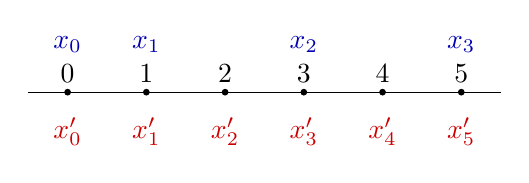
\begin{tikzpicture}
    \draw (0,0) -- (6,0);
    \filldraw[black] (0.5,0) circle (1pt) node[anchor=south]{0};
    \filldraw[black] (1.5,0) circle (1pt) node[anchor=south]{1};
    \filldraw[black] (2.5,0) circle (1pt) node[anchor=south]{2};
    \filldraw[black] (3.5,0) circle (1pt) node[anchor=south]{3};
    \filldraw[black] (4.5,0) circle (1pt) node[anchor=south]{4};
    \filldraw[black] (5.5,0) circle (1pt) node[anchor=south]{5};
    \filldraw[blue!70!black] (0.5,0.6) node[]{$x_{0}$};
    \filldraw[blue!70!black] (1.5,0.6) node[]{$x_{1}$};
    \filldraw[blue!70!black] (3.5,0.6) node[]{$x_{2}$};
    \filldraw[blue!70!black] (5.5,0.6) node[]{$x_{3}$};
    \filldraw[red!80!black] (0.5,-0.5) node[]{$x'_{0}$};
    \filldraw[red!80!black] (1.5,-0.5) node[]{$x'_{1}$};
    \filldraw[red!80!black] (2.5,-0.5) node[]{$x'_{2}$};
    \filldraw[red!80!black] (3.5,-0.5) node[]{$x'_{3}$};
    \filldraw[red!80!black] (4.5,-0.5) node[]{$x'_{4}$};
    \filldraw[red!80!black] (5.5,-0.5) node[]{$x'_{5}$};
\end{tikzpicture}

    $ k = 5, \tau' = \{ [0; 1], [1; 2], [2; 3], [3; 4], [4; 5] \} $

    $ x'_0 = 0, x'_1 = 1, x'_2 = 2, x'_3 = 3, x'_4 = 4, x'_5 = 5 $
}

\mcdfn{Диаметр разбиения}{
    Диаметр разбиения - это $ d(\tau) 
        = \underset{1 \le i \le n}{\max} (x_i - x_{i - 1}) 
        = \underset{1 \le i \le n}{\max} \Delta x_i $
}

\mcdfn{Разметка разбиения}{
    Разметка разбиения - это множество $ \{ \xi_i | \xi_i \in [x_{i - 1}; x_i] \}_{i = 1}^{n} $

    Разбиение, у которого есть разметка, называется размеченным разбиением
}

\subsection{Интегральная сумма Римана}

\mcdfn{Интегральная сумма Римана}{
    Интегральная сумма (Римана) - это \[ \sigma_{\tau}(f) = \sum_{i = 1}^{n} f(\xi_i) \Delta x_i \]
}

\subsection{Определение определённого интеграла по Коши}

\label{cauchy_integr_def:3}

\mcdfn{Определение определённого интеграла по Коши}{
    Число $I$ называется определённым интегралом $f(x)$ на $[a; b]$, если

    $ \forall \veps > 0 \,
        \exists \delta > 0 \,
        \forall \tau: d(\tau) < \delta \,
        \forall \text{ разметки } \{ \xi_i \}_{i = 1}^{n}: \,
        | \sigma_\tau(f) - I | < \veps $
}

\subsection{Определение определённого интеграла по Гейне}

\mcdfn{Определение определённого интеграла по Гейне}{
    Число $I$ называется определённым интегралом $f(x)$ на $[a; b]$, если

    $ \forall \text{ послед. } \tau_k: d(\tau_k) \underset{k \to +\infty}{\to} 0 \,
        \forall \{ \xi_{i}^{k} \}_{i = 1}^{n}: \,
        \sigma_{\tau_k}(f) \underset{k \to +\infty}{\to} I $
}

\subsection{Определение функции, интегрируемой по Риману}

\mcdfn{Определение интегрируемости по Риману}{
    Функция $f(x)$ интегрируема по Риману, если $\exists I \in \Rset[] $, т.ч.
    выполняется определение по Коши $\ref{cauchy_integr_def:3}$

    Обозначения: 

    $ f(x) \in R[a; b] $, где $R[a; b]$ - множество функций, интегрируемых по Риману на отрезке $[a; b]$

    $ I = \int_{a}^{b} f(x) dx $
}

\mcex{}{
    Пример функции, не интегрируемой по Риману:

    На отрезке $[0; 1]$ рассмотрим функцию Дирихле: 
    $ D(x) = \left\{ \begin{tabular}{l}
        $ 1, x \in \Qset $ \\
        $ 0, x \notin \Qset $ \\
    \end{tabular} \right. $

    Выберем первую разметку такую, что $ \forall i \in \{ 1, ..., n \}: \xi_i \in \Qset $

    Тогда $ \sigma_{\tau}(D) 
        = \sum_{i = 1}^{n} D(\xi_i) \Delta x_i 
        = \sum_{i = 1}^{n} \Delta x_i = b - a = 1 - 0 = 1 $

    Выберем вторую разметку такую, что $ \forall i \in \{ 1, ..., n \}: \xi_i \in \Rset \setminus \Qset $

    Тогда $ \sigma_{\tau}(D) 
        = \sum_{i = 1}^{n} D(\xi_i) \Delta x_i 
        = \sum_{i = 1}^{n} 0 \cdot \Delta x_i = 0 $
}

\subsection{Теорема об ограниченности функции, интегрируемой на отрезке}

\mcthm{Теорема об ограниченности функции, интегрируемой на отрезке}{
    Функция, $f(x)$ интегрируемая на $ [a; b] $, ограничена на $ [a; b] $

\mcprf{
\begin{split}
    & \text{1. Предположим от противного, т.е. функция не ограничена на отрезке} \\
    & \text{По определению интегрируемости для } \veps = 1: \\
    & \exists \delta > 0 \, 
        \forall \tau: d(\tau) < \delta \, 
        \forall \{ \xi_i \}_{i = 1}^{n}: \,
        | \sigma_\tau(f) - I | < 1\\
    & \text{Зафиксируем $\tau$. Хотя бы на 1 элементе $ \tau $ $f(x)$ не ограничена. БОО это первый отрезок $[x_0; x_1]$} \\
    & \text{Зафиксируем разметку везде кроме 1-ого отрезка: } \xi_2, \xi_2, ... \xi_n \\
    & | \sigma_\tau(f) | - | I | \le | \sigma_\tau(f) - I | \implies | \sigma_\tau(f) | < | I | + 1 \\
    & | f(\xi_1) | \Delta x_1 - \sum_{i = 2}^{n} | f(\xi_i) | \Delta x_i \le | \sigma_\tau(f) | 
        \implies | f(\xi_1) | \Delta x_1 < | I | + 1 + \sum_{i = 2}^{n} | f(\xi_i) | \Delta x_i \\
    & | f(\xi_1) | < \frac{| I | + 1 + \sum_{i = 2}^{n} | f(\xi_i) | \Delta x_i}{\Delta x_1} \\
    & \text{Обозначим } C = \frac{| I | + 1 + \sum_{i = 2}^{n} | f(\xi_i) | \Delta x_i}{\Delta x_1} > 0 \\
    & \text{Получили: } \forall \xi_1 \in [x_0; x_1]: | f(\xi_1) | < C \\
    & \text{Но на отрезке $[x_0; x_1]$ функция не ограничена } \implies \Contradiction \\
\end{split}
}
}

\subsection{Суммы Дарбу}

\subsubsection{Нижняя сумма Дарбу}

\mcdfn{Нижняя сумма Дарбу}{
    Пусть $ f(x) $ ограничена на $ [a; b] $, дано разбиение $ \tau $, 
    тогда нижней суммой Дарбу называется

    $ s_\tau = \sum_{i = 1}^{n} m_i \Delta x_i $, 
    где $ \forall i: m_i = \underset{x \in [x_{i - 1}; x_i]}{\inf} f(x) $
}

\subsubsection{Верхняя сумма Дарбу}

\mcdfn{Верхняя сумма Дарбу}{
    Пусть $ f(x) $ ограничена на $ [a; b] $, дано разбиение $ \tau $, 
    тогда верхней суммой Дарбу называется

    $ S_\tau = \sum_{i = 1}^{n} M_i \Delta x_i $, 
    где $ \forall i: M_i = \underset{x \in [x_{i - 1}; x_i]}{\sup} f(x) $
}

\subsubsection{Свойства сумм Дарбу}

\label{darboux_sums_props:4}

\mcclm{Свойства сумм Дарбу}{}{
\begin{tabular}{rl}
    $\bullet$ & $ s_\tau, S_\tau $ определены, если $ f(x) $ ограничена, 
                    т.е. $ s_\tau \in \Rset[] \wedge S_\tau \in \Rset[] $ \\
    $\bullet$ & Если $ \tau' \succ \tau $, то: \\
              & $ S_{\tau'} \le S_\tau $ \\
              & $ s_{\tau'} \ge s_\tau $ \\
    $\bullet$ & $ \forall \tau_1, \tau_2: s_{\tau_1} \le S_{\tau_2} $ \\
    $\bullet$ & $ s_\tau = \underset{ \{ \xi_i \}_{i = 1}^{n} }{\inf} \sigma_{\tau}(f) $ - инфинум по всем разметкам \\
              & $ S_\tau = \underset{ \{ \xi_i \}_{i = 1}^{n} }{\sup} \sigma_{\tau}(f) $ - супремум по всем разметкам \\
\end{tabular}

    Докажем 2-е свойство для нижних сумм Дарбу:
\mcprf{
\begin{split}
    & \text{Докажем для нижних сумм, для верхних сумм аналогично: } \\
    & s_\tau = \sum_{i = 1}^{n} m_i \Delta x_i \\
    & s_{\tau'} = \sum_{j = 1}^{k} m'_j \Delta x'_j \\
    & \forall i \, \exists n_{i - 1} < n_i: 
        \sum_{j = n_{i - 1} + 1}^{n_i} \Delta x'_j = \Delta x_i 
        \text{ и } 
        \cup_{j = n_{i - 1} + 1}^{n_i} [x'_{j - 1}; x'_j] = [x_{i - 1}; x_i] \\
    & 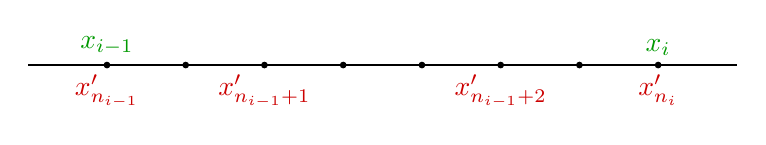
\begin{tikzpicture}
        \draw (0,0) -- (9,0);
        \filldraw[black] (1,0) circle (1pt);
        \filldraw[black] (2,0) circle (1pt);
        \filldraw[black] (3,0) circle (1pt);
        \filldraw[black] (4,0) circle (1pt);
        \filldraw[black] (5,0) circle (1pt);
        \filldraw[black] (6,0) circle (1pt);
        \filldraw[black] (7,0) circle (1pt);
        \filldraw[black] (8,0) circle (1pt);
        \filldraw[green!60!black] (1,0) node[anchor=south]{$x_{i-1}$};
        \filldraw[green!60!black] (8,0) node[anchor=south]{$x_{i}$};
        \filldraw[red!80!black] (1,0) node[anchor=north]{$x'_{n_{i - 1}}$};
        \filldraw[red!80!black] (3,0) node[anchor=north]{$x'_{n_{i - 1} + 1}$};
        \filldraw[red!80!black] (6,0) node[anchor=north]{$x'_{n_{i - 1} + 2}$};
        \filldraw[red!80!black] (8,0) node[anchor=north]{$x'_{n_i}$};
    \end{tikzpicture} \\
    & \text{Т.к. $m_i$ - $\inf f(x)$ на всём отрезке $[x_{i-1}; x_i]$, то } \forall j \in \{ n_{i - 1} + 1, ..., n_i \}: m'_j \ge m_i \\
    & \text{Тогда } m'_j \Delta x'_j \ge m_i \Delta x'_j \\
    & \text{Следовательно, } \sum_{j = n_{i - 1} + 1}^{n_i} m'_j \Delta x'_j 
        \ge \sum_{j = n_{i - 1} + 1}^{n_i} m_i \Delta x'_j 
        = m_i \Delta x_i \\
    & \text{Тогда } 
        \sum_{j = 1}^{k} m'_j \Delta x'_j \ge \sum_{i = 1}^{n} m_i \Delta x_i 
        \implies
        s_\tau' \ge s_\tau \\
\end{split}
}

    Докажем 3-е свойство:
\mcprf{
\begin{split}
    & \text{Рассмотрим разбиение $ \tau $, состоящее из точек $ \tau_1 $ и $ \tau_2 $, тогда }
        \tau \succ \tau_1, \tau_2 \\
    & \text{Следовательно, по 2-му свойству сумм Дарбу: } s_{\tau_1} \le s_{\tau} \le S_\tau \le S_{\tau_2} \\
\end{split}
}

    Докажем 4-е свойство:
\mcprf{
\begin{split}
    & s_\tau
        = \sum_{i = 1}^{n} \underset{\xi_i \in [x_{i - 1}; x_i]}{\inf f(\xi_i)} \Delta x_i 
        = \underset{ \{ \xi_i \}_{i = 1}^{n} }{\inf} \sum_{i = 1}^{n} f(\xi_i) \Delta x_i
        = \underset{ \{ \xi_i \}_{i = 1}^{n} }{\inf} \sigma_{\tau}(f) \\
\end{split}
}
}

\subsubsection{Интегралы Дарбу}

\mcdfn{Верхний интеграл Дарбу}{
    Верхним интегралом Дарбу называется $ I^* = \underset{\tau}{\inf} S_{\tau} $ - инфинум верхних сумм Дарбу по всем разбиениям
}

\mcdfn{Нижний интеграл Дарбу}{
    Нижним интегралом Дарбу называется $ I_* = \underset{\tau}{\sup} s_{\tau} $ - супремум нижних сумм Дарбу по всем разбиениям
}

\mcclarf{Уточнение}{
    $ s_\tau \le S_\tau \implies I_* \le I^* $
}

\subsection{Критерий Дарбу интегрируемости по Риману}

\mclemma{Лемма 1}{
    Пусть $ \tau' \succ \tau $ и у $ \tau' $ на p точек (т.е. границ отрезков) больше, чем у $\tau$

    Тогда $ 0 \le S_{\tau} - S_{\tau'} \le (M - m) \cdot p \cdot \delta $, 
        где $ \delta > d(\tau) $, 
            $ m = \underset{x \in [a; b]}{\inf} f(x) \in \Rset[] $,
            $ M = \underset{x \in [a; b]}{\sup} f(x) \in \Rset[] $
\mcproofpure{
\[
\begin{split}
    & \text{1. $S_{\tau} - S_{\tau'} \ge 0 $ по свойству 2 сумм Дарбу \ref{darboux_sums_props:4}} \\
    & \text{2. Рассмотрим случай, когда $p = 1$} \\
    & \text{ Пусть граница отрезка, которая есть в $\tau'$, но которой нет в $\tau$, имеет индекс $i$ } \\
    & 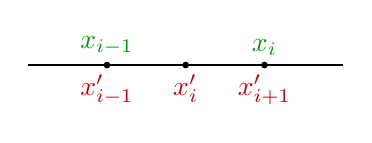
\begin{tikzpicture}
        \draw (0,0) -- (4,0);
        \filldraw[black] (1,0) circle (1pt);
        \filldraw[black] (2,0) circle (1pt);
        \filldraw[black] (3,0) circle (1pt);
        \filldraw[green!60!black] (1,0) node[anchor=south]{$x_{i-1}$};
        \filldraw[green!60!black] (3,0) node[anchor=south]{$x_{i}$};
        \filldraw[red!80!black] (1,0) node[anchor=north]{$x'_{i-1}$};
        \filldraw[red!80!black] (2,0) node[anchor=north]{$x'_{i}$};
        \filldraw[red!80!black] (3,0) node[anchor=north]{$x'_{i+1}$};
    \end{tikzpicture} \\
    & S_{\tau} = \sum_{j = 1}^{n} M_j \textcolor{green!60!black}{\Delta x_j} 
        \text{, где } M_j = \underset{x \in [\textcolor{green!60!black}{x_{j-1}}; \textcolor{green!60!black}{x_j}]}{\sup f(x)} \\
    & S_{\tau'} = \sum_{j = 1}^{n + 1} M'_j \textcolor{red!80!black}{\Delta x'_j}
        \text{, где } M'_j = \underset{x \in [\textcolor{red!80!black}{x'_{j-1}}; \textcolor{red!80!black}{x'_j}]}{\sup f(x)} \\
    & \text{Причём } 
        \forall j < i: \textcolor{green!60!black}{x_j} = \textcolor{red!80!black}{x'_j} \wedge M_j = M'_j 
        \text{ и } 
        \textcolor{green!60!black}{x_i} = \textcolor{red!80!black}{x'_{i+1}}
        \text{ и } 
        \forall j > i: \textcolor{green!60!black}{x_{j}} = \textcolor{red!80!black}{x'_{j + 1}} \wedge M_{j} = M'_{j + 1} \\
    & \text{Тогда } S_\tau - S_{\tau'} 
        = M_i \textcolor{green!60!black}{\Delta x_i} 
        - (M'_i \textcolor{red!80!black}{\Delta x'_i} + M'_{i + 1} \textcolor{red!80!black}{\Delta x'_{i + 1}}) 
        = M_i (\textcolor{red!80!black}{\Delta x'_i} + \textcolor{red!80!black}{\Delta x'_{i + 1}}) 
        - (M'_i \textcolor{red!80!black}{\Delta x'_i} + M'_{i + 1} \textcolor{red!80!black}{\Delta x'_{i + 1}})
        = \\
    &   = (M_i - M'_i) \textcolor{red!80!black}{\Delta x'_i} + (M_i - M'_{i+1}) \textcolor{red!80!black}{\Delta x'_{i + 1}}
        \le \left| \text{т.к. $M_i \le M$ и $M'_i \ge m$} \right|
        \le (M - m) \textcolor{red!80!black}{\Delta x'_i} + (M - m) \textcolor{red!80!black}{\Delta x'_{i + 1}} = \\
    &   = (M - m) \textcolor{green!60!black}{\Delta x_i} \le (M - m) \cdot d(\tau) < (M - m) \cdot \delta \\
\end{split}
\]

3. Для p > 1 доказывается итерационно, сводя для каждой из $p$ точек измельчения $\tau'$ к пункту 2.
}
}

\mclemma{Лемма Дарбу}{
    Пусть дан отрезок $[a; b]$ и функция $f(x)$, непрерывная на отрезке $[a; b]$, тогда

    \[ I^* = \lim_{d \to 0} S_{\tau} \]

    Это означает, что $ \forall \veps > 0 \, \exists \delta > 0 \, \forall \tau: d(\tau) < \delta: | S_\tau - I^* | < \veps $
\mcprf{
\begin{split}
    & \text{1. Если $m = M$, то функция - константа на отрезке $[a; b]$, тогда все верхние суммы равны} \\
    & \text{$ f(a) \cdot (b - a) \implies I^* = f(a) \cdot (b - a)$, т.к. $I^*$ - это инфинум верхних сумм по всем разбиениям} \\
    & \text{2. Иначе, если $m \ne M$, то $m < M$} \\
    & \text{Пусть дано $\veps > 0$, тогда} \\
    & I^* = \underset{\tau}{\inf S_\tau} \implies \exists \tau^*: \left| S_{\tau^*} - I^* \right| < \frac{\veps}{2} \\
    & \text{$I^*$ - инфинум всех верхних сумм } \implies S_{\tau^*} \ge I^* \implies S_{\tau^*} - I^* < \frac{\veps}{2} \\
    & \text{Пусть в $\tau^*$ p точек (границ отрезков внутри $(a; b)$), т.е. $\tau^*$ состоит из $p+1$ отрезка } \\
    & \text{Положим } \delta = \frac{\veps}{2 (M - n) p} \\
    & \text{Построено $\delta$, тогда пусть дано разбиение $\tau$ т.ч. $d(\tau) < \delta$} \\
    & \text{Составим разбиение $\tau'$ из границ отрезков разбиений $\tau$ и $\tau^*$, тогда $ \tau' \succ \tau \wedge \tau' \succ \tau^* $,}\\
    & \text{и при этом в $\tau'$ не более чем на $p$ больше точек (границ отрезков), чем в $\tau$, тогда по Лемме 1} \\
    & 0 \le S_\tau - S_{\tau'} \le (M - m) \cdot p \cdot \delta = \frac{\veps}{2} \\
    & \text{(если в $\tau'$ меньше, чем на p больше точек, чем в $\tau$, то неравенство также выполняется)} \\
    & \text{$\tau'$ - измельчение $\tau^*$ по построению } \implies S_{\tau'} \le S_{\tau^*} \\
    & \text{$I^*$ - инфинум всех верхних сумм } \implies S_{\tau'} \ge I^* \implies I^* \le S_{\tau'} \le S_{\tau^*} \\
    & S_{\tau^*} - I^* < \frac{\veps}{2} \implies S_{\tau'} - I^* < \frac{\veps}{2} \\
    & \left. \begin{tabular}{l}
        $ 0 \le S_\tau - S_{\tau'} < \frac{\veps}{2} $ \\
        $ 0 \le S_{\tau'} - I^* < \frac{\veps}{2} $ \\
    \end{tabular} \right\} \implies 0 \le S_\tau - I^* < \veps \implies \left| S_\tau - I^* \right| < \veps \\
\end{split}
}
}

\nt{
    Аналогичная лемма верна и для случая нижних сумм: \[ I_* = \lim_{d \to 0} s_{\tau} \]
}

\mcthm{Критерий Дарбу интегрируемости по Риману}{
    Ограниченная функция $ f(x) $ интегрируема на $ [a; b] \iff I^* = I_* $

    Используя введённые обозначения, $f(x) \in R[a; b] \iff f(x) \text{ ограничена и } I^* = I_*  $

\mcprf{
\begin{split}
    & "\implies" \\
    & \text{Предположим от противного, т.е. функция интегрируема и } I_* \ne I^* \implies I_* < I^* \\
    & \text{По определению интегрируемости:} \\
    & \forall \veps > 0 \, 
        \exists \delta > 0 \, 
        \forall \tau: d(\tau) < \delta 
        \forall \{ \xi_i \}_{i = 1}^{n}: \,
        | \sigma_\tau(f) - I | < \veps \\ 
    & | \sigma_\tau(f) - I | < \veps 
        \implies I - \veps < \sigma_\tau(f) < I + \veps 
        \implies I - \veps \le s_\tau \le S_\tau \le I + \veps \text{ по сво-ву 4} \\
    & s_\tau \le I_* < I^* \le S_\tau \implies S_\tau - s_\tau \ge I^* - I_* > 0
        \text{, но при этом } \forall \veps > 0: S_\tau - s_\tau \le 2 \veps 
        \implies \Contradiction \\
    & "\impliedby" \\
    & \text{Обозначим $I = I_* = I^*$ и покажем, что выполняется определение, т.е.}  \\
    & \forall \veps > 0 \, \exists \delta > 0 \, \forall \tau: d(\tau) < \delta \, \forall \{ \xi_i \}_{i = 1}^{n}: | \sigma_\tau(f) - I | < \veps \\
    & | \sigma_\tau(f) - I | < \veps \implies I - \veps < \sigma_\tau(f) < I + \veps \\
    & \text{По определению сумм Дарбу } s_\tau \le \sigma_\tau(f) \le S_\tau \\
    & \text{По лемме Дарбу $ \exists \delta_1 > d(\tau):  S_\tau < I^* + \veps $} \\
    & \text{аналогично $ \exists \delta_2 > d(\tau): s_\tau > I_* - \veps $} \\
    & \text{Положим $\delta = \min(\delta_1, \delta_2)$, тогда: } 
        I_* - \veps 
        < \sigma_\tau(f) 
        < I^* + \veps \implies I - \veps 
        < \sigma_\tau(f) 
        < I^* + \veps 
        = I + \veps \\
\end{split}
}
}

\subsection{Определение равномерной непрерывности}

\mcdfn{Определение равномерной непрерывности}
{
    Функция $f(x)$ называется равномерно непрерывной на $E \subseteq \Rset[] $, если

    $ \forall \veps > 0 \, \exists \delta = \delta(\veps) > 0 \, \forall x_1, x_2 \in E: | x_1 - x_2 | < \delta \implies | f(x_1) - f(x_2) | < \veps $
}

\nt{
    $f(x)$ равномерно непрерывна на $E \implies f(x)$ непрерывна на $E$, но обратное, вообще говоря, не верно
}

\mcex{Пример к замечанию}{
    $ E = (0; 1), f(x) = \frac{1}{x} $

    $f(x)$ непрерывна на $E$, покажем, что равномерной непрерывности нет:

    Рассмотрим последовательность аргументов: $x_n = \frac{1}{n}$, тогда $x_{n+1} - x_n \underset{n \to +\infty}{\to} 0 $,

    но при этом $f(x_{n+1}) - f(x_n) = 1$

    Положим $\veps = 0.5$, тогда т.к. $x_{n+1} - x_n \underset{n \to +\infty}{\to} 0 $, то можно выбрать $x_i$ и $x_j$, т.ч. $|x_i - x_j| < \delta(0.5)$,
    но при этом $ |f(x_1) - f(x_2)| = 1 > 0.5 = \veps $
}

\subsection{Теорема Кантора}

\mcthm{Теорема Кантора (для случая функции на отрезке)}{
    Если $f(x)$ непрерывна на $[a; b]$, то $f(x)$ равномерно непрерывна на $[a; b]$
\mcprf{
\begin{split}
    & \text{Предположим от противного, тогда в отрицании определения выберем конкретные значения $\delta$:} \\
    & \exists \veps_0 \, \forall \delta = \frac{1}{n} \, \exists x'_n, x_n'' \in [a; b]: | x'_n - x''_n | < \frac{1}{n}: \left| f\left(x'_n\right) - f\left(x''_n\right) \right| > \veps_0 \\
    & \text{Ч.п. $\{ x'_n \}$ и $\{ x''_n \}$ ограничены $\implies$ по теореме Больцано-Вейерштрасса из них можно } \\
    & \text{выделить сходящиеся подпоследовательности: } \exists x'_{n_k} \underset{k \to +\infty}{\to} x_0 \in [a; b] \\
    & \text{При этом по теореме о зажатой последовательности } x''_{n_k} \underset{k \to +\infty}{\to} x_0 \\
    & \text{$f(x)$ непрерывна в точке $x_0$, тогда по определению непрерывности в точке по Гейне:} \\
    & f\left(x'_{n_k}\right) \underset{k \to +\infty}{\to} f(x_0) \\
    & f\left(x''_{n_k}\right) \underset{k \to +\infty}{\to} f(x_0) \\
    & \text{Но по предположению } \left| f\left(x'_n\right) - f\left(x''_n\right) \right| > \veps_0 \implies \Contradiction \\
\end{split}
}
}

\subsection{Теорема об интегрируемости непрерывной функции}

\mcthm{Теорема об интегрируемости непрерывной функции}{
    Если $f(x)$ непрерывна на $[a; b]$, то $f(x) \in R[a; b]$

\mcprf{
\begin{split}
    & 1. f(x) \text{ непрерывна на } [a; b] \implies \text{ по теореме Кантора $f(x)$ равномерно непрерывна на } \\
    & [a; b] \text{, тогда по определению: } 
        \forall \veps > 0 \, 
        \exists \delta > 0 \, 
        \forall x_1, x_2 \in [a; b]: 
        | x_1 - x_2 | < \delta \implies | f(x_1) - f(x_2) | < \veps \\
    & \text{2. Для любого $\veps > 0$ рассмотрим разбиение $\tau$ отрезка $[a; b]$ с диаметром $d(\tau) < \delta$, тогда} \\
    &   0 \le I^* - I_* 
        \le S_\tau - s_\tau 
        = \sum_{i = 1}^{n} \left(M_i - m_i\right) \Delta x_i
        = \sum_{i = 1}^{n} \left(f(\xi_i) - f(\eta_i)\right) \Delta x_i \text{, т.к. $f$ непрерывна на $[a; b]$} \\
    & \forall i: | \xi_i - \eta_i | \le d(\tau) < \delta \implies |f(\xi_i) - f(\eta_i)| < \veps \implies 0 \ge f(\xi_i) - f(\eta_i) < \veps \\
    & \text{Тогда } 
        \sum_{i = 1}^{n} \left(f(\xi_i) - f(\eta_i)\right) \Delta x_i  \le \sum_{i = 1}^{n} \veps \Delta x_i = \veps \cdot (b - a) \\
    & \text{$I^* - I_*$ - неотрицательное число, и при этом } \forall \veps > 0: I^* - I_* < \veps (b - a) \implies I^* - I_* = 0 \\
\end{split}
}
}

\subsection{Теорема об интегрируемости монотонной функции}

\mcthm{Теорема об интегрируемости монотонной функции}{
    Если $f(x)$ определена и монотонна на $[a; b]$, то $f(x) \in R[a; b]$
\mcprf{
\begin{split}
    & \text{БОО докажем для неубывающей функции} \\
    & \text{1. Для любого $\delta > 0$ рассмотрим разбиение $\tau$ отрезка $[a; b]$ с диаметром $d(\tau) < \delta$, тогда} \\
    & 0 \le I^* - I_* 
        \le S_\tau - s_\tau 
        = \sum_{i = 1}^{n} \left(M_i - m_i\right) \Delta x_i
        = \sum_{i = 1}^{n} \left(f(x_i) - f(x_{i-1})\right) \Delta x_i
        < \sum_{i = 1}^{n} \left(f(x_i) - f(x_{i-1})\right) \delta 
        = \\
    &   = \delta \sum_{i = 1}^{n} \left(f(x_i) - f(x_{i-1})\right) 
        = \delta \left(f(b) - f(a)\right) \\
    & \text{$I^* - I_*$ - неотрицательное число, и при этом } \forall \delta > 0: I^* - I_* < \delta \left(f(b) - f(a)\right) \implies I^* - I_* = 0 \\
\end{split}
}
}

\subsection{Элементы теории меры}

\subsubsection{Критерий Лебега интегрируемости по Риману}

\mcthm{Критерий Лебега интегрируемости по Риману (без док-ва)}{
    Функция $f(x) \in R[a; b] \iff $ функция $f(x)$ ограничена и множество точек разрыва функции - множество меры ноль по Лебегу
}

\subsubsection{Определение множества меры ноль по Лебегу}

\mcdfn{Определение множества меры ноль по Лебегу}{
    Множество $E \subseteq \Rset[] $ называется множеством нулевой меры Лебега, если

    $ \forall \veps > 0 \, \exists \text{ не более чем счётный набор интервалов } \{ (a_i; b_i) \}_{i = 1}^{+\infty} $, такой что

    1. $ E \subseteq \cup_{i = 1}^{+\infty} (a_i; b_i) $, т.е. объединение всех интервалов покрывает множество $E$

    2. $ \sum_{i = 1}^{+\infty} b_i - a_i \le \veps $

    Обозначение: $ \mu(E) = 0 $
}

\mcex{Пример множества меры ноль по Лебегу}{
    Покажем, что $ \Qset[] \subseteq \Rset[] $ - множество нулевой меры Лебега
\mcprf{
\begin{split}
    & \text{1. } \Qset[] \cong \Nset[] \implies \Qset[] = \{ q_i \}_{i = 1}^{+\infty} \\    
    & \text{2. } \forall i \in \Nset[]: (a_i; b_i) = U_\frac{\veps}{2^{i+1}}(q_i) \implies \Qset[] \subseteq \cup_{i = 1}^{+\infty} (a_i; b_i) \\
    & \text{3. При этом } \sum_{i = 1}^{+\infty} b_i - a_i = \sum_{i = 1}^{+\infty} 2 \cdot \frac{\veps}{2^{i+1}} = \veps \le \veps \\
\end{split}
}
}

\subsubsection{Свойства множеств меры ноль по Лебегу}

\mcthm{Свойства множеств меры ноль по Лебегу}{
\begin{tabular}{rl}
    1. & Если $A \subseteq \Rset[]$ нулевой меры Лебега и 
        $B \subseteq A$, то $B$ тоже множество нулевой меры Лебега \\
       & (это свойство меры называется полнотой) \\
    2. & Если множества $X, Y$ - нулевой меры Лебега, то $X \cup Y$ - нулевой меры Лебега \\
\end{tabular}

Докажем 1-е свойство:
\mcprf{
\begin{split}
    & \text{$\forall \veps > 0$ по определению множества меры ноль по Лебегу построим покрытие} \\
    & \text{ множества $A: \{ (a_i; b_i) \}_{i=1}^{+\infty} $, т.ч. $\sum_{i = 1}^{+\infty} b_i - a_i \le \veps$} \\
    & \text{$B \subseteq A \implies B \subseteq \cup_{i = 1}^{+\infty} (a_i; b_i)$} \\
\end{split}
}

Докажем 2-е свойство:
\mcprf{
\begin{split}
    & \text{Пусть дано $\veps > 0$, тогда:} \\
    & \text{Для $\frac{\veps}{2}$ по определению множества нулевой меры Лебега построим покрытия } \\
    & \text{для множеств $X$ и $Y$: } \{(a_i; b_i)\}_{i = 1}^{+\infty} \text{ и } \{(c_i; d_i)\}_{i = 1}^{+\infty} \text{ соответственно} \\
    & \text{Тогда для множества $X \cup Y$ построим покрытие } \{(e_i; f_i)\}_{i = 1}^{+\infty} \text{ такое что} \\
    & e_i = \left\{ \begin{tabular}{l}
        $ a_j, i = 2 j $ \\
        $ c_j, i = 2 j + 1 $ \\
    \end{tabular} \right. \\
    & f_i = \left\{ \begin{tabular}{l}
        $ b_j, i = 2 j $ \\
        $ d_j, i = 2 j + 1 $ \\
    \end{tabular} \right. \\
    & \text{Тогда $ X \cup Y \subseteq \cup_{i=1}^{+\infty} (e_i; f_i) $ и: } \\
    & \sum_{i=1}^{+\infty} \left| f_i - e_i \right|
    = \sum_{j=1}^{+\infty} | b_j - a_j | + \sum_{j=1}^{+\infty} | d_j - c_j |
    \le \frac{\veps}{2} + \frac{\veps}{2}
    = \veps \\
\end{split}
}
}

\nt{
    Из 1 и 2 свойств следует, что разность, пересечение и 
    симметрическая разность множеств нулевой меры Лебега -
    также множества нулевой меры Лебега
}

\subsection{Свойства определённого интеграла}

\mcthmBreakable{Свойства определённого интеграла}{
\begin{tabular}{rl}
    1.  & Линейность: \\
        & Пусть $ f, g \in R[a; b] $, тогда \\
        & $
        \forall \alpha, \beta \in \Rset[]: \alpha f + \beta g \in R[a; b] 
        \wedge \int_{a}^{b} \left( \alpha f(x) + \beta g(x) \right) dx 
        = \alpha \int_{a}^{b} f(x) dx + \beta \int_{a}^{b} g(x) dx 
        $\\
    2.  & Если $f, g \in R[a; b]$, то $ f \cdot g \in R[a; b] \wedge | f | \in R[a; b] $ \\
        & (здесь $f \cdot g$ - это произведение, а не композиция, т.е. $\forall x \in \Rset: (f \cdot g)(x) = f(x) \cdot g(x) $) \\
    3.  & Аддетивность: если $f \in R[a; c]$, и $b \in [a; c]$ 
        то: \\
        & $f \in R[a; b] \cup R[b; c] $ и 
            $ \int_{a}^{c} f(x) dx 
            = \int_{a}^{b} f(x) dx 
            + \int_{b}^{c} f(x) dx $ \\
    4.  & Интегрируемось неравенств: 
            $f, g \in R[a; b]$ и 
            $ \forall x \in [a; b]: f(x) \le g(x) $, то:\\
        & $ \int_{a}^{b} f(x) dx \le \int_{a}^{b} g(x) dx $ \\ 
    5.  & Теорема о среднем: \\
        & Если $f(x)$ непрерывна на $[a; b]$, то
            $ \exists \xi \in [a; b]: 
            f(\xi) = \frac{1}{b - a} \int_{a}^{b} f(x) dx $ \\
    6.  & Оценка интеграла: \\
        & Если $f(x) \in R[a; b]$, то: \\
        & $ \left| \int_{a}^{b} f(x) dx \right| 
            \le \int_{a}^{b} \left| f(x) \right| dx $  \\
\end{tabular}

Докажем 1-е свойство:
\mcprf{
\begin{split}
    & \text{1. По критерию Лебега интегрируемости по Риману: $ f, g $ - ограниченные на $[a;b]$ функции и} \\
    & X_f \text{ - множество точек разрыва функции $f$ и при этом $\mu(X_f) = 0$} \\
    & X_g \text{ - множество точек разрыва функции $g$ и при этом $\mu(X_g) = 0$} \\
    & \text{Пусть $ X_{\alpha f + \beta g} $ - множество точек разрыва непрерывной на $[a;b]$ функции $\alpha f + \beta g$} \\
    & X_{\alpha f + \beta g} \subseteq X_f \cup X_g \implies \mu(X_{\alpha f + \beta g}) = 0 \\
    & \text{Тогда по критерию Лебега интегрируемости по Риману $ \alpha f + \beta g \in R[a; b] $} \\
    & \text{2. Рассмотрим последовательность разбиений $\tau_k$:} 
        \forall \tau_k
        \forall \{ \xi_i \}_{i=1}^{+\infty} 
        \sigma_{\tau}(\alpha f + \beta g) 
            = \alpha \sigma_{\tau}(f) + \beta \sigma_{\tau}(g) \text{, т.к.} \\
    &   \sigma_{\tau}(\alpha f + \beta g)
        = \sum_{i=1}^{n} \left( \alpha f(\xi_i) + \beta g(\xi_i) \right) \cdot \Delta x_i
        = \sum_{i=1}^{n} \alpha f(\xi_i) \cdot \Delta x_i + \sum_{i=1}^{n} \beta g(\xi_i) \cdot \Delta x_i 
        = \alpha \sigma_{\tau}(f) + \beta \sigma_{\tau}(g) \\
    & \text{По определению Гейне интегрируемости по Риману:} \\
    & \sigma_{\tau}(\alpha f + \beta g) \underset{k \to +\infty}{\to} 
        \int_{a}^{b} \left(\alpha f(x) + \beta g(x)\right) dx \\
    & \alpha \sigma_{\tau}(f) \underset{k \to +\infty}{\to} 
        \alpha \int_{a}^{b} f(x) dx \\
    & \beta \sigma_{\tau}(g) \underset{k \to +\infty}{\to} 
        \beta \int_{a}^{b} g(x) dx \\
    & \implies \int_{a}^{b} \left(\alpha f(x) + \beta g(x)\right) dx 
        = \alpha \int_{a}^{b} f(x) dx + \beta \int_{a}^{b} g(x) dx \\
\end{split}
}

2-е свойство:
\begin{equation*}
\begin{split}
    & \text{2-е свойство доказывается аналогично 1-ому доказательству, т.к. множества точек разрыва } \\
    & \text{функций $f \cdot g$ и $|f|$ - множества меры ноль по Лебегу и эти функции непрерывны на $[a; b]$ } \\
    & \text{ } \\
\end{split}
\end{equation*}

Докажем 3-е свойство:
\mcprf{
\begin{split}
    & \text{1. $f \in R[a; c] \implies$ и на отрезках $[a; b]$ и $[b; c]$ 
        она непрерывна и её множества точек разрыва } \\
    & \text{ на этих отрезках тоже множества меры ноль по Лебегу } 
            \implies f \in R[a; b] \wedge f \in R[b; c] \\
    & \text{2. По определению интегрируемости по Гейне: } \\
    & \forall \tau_k \text{ разбиения отрезка $[a;c]$ т.ч. }
        d(\tau_k) \underset{k \to +\infty}{\to} 0 \,
        \forall \{ \xi_i^k \}_{i=1}^{n}:
        \sigma_{\tau_k}(f) 
        = \sum_{i=1}^{n} f(\xi_i^k)\Delta x^k 
        \underset{k \to +\infty}{\to} 
        \int_{a}^{c} f(x) dx \\
    & \text{Будем рассматривать последовательность $ \tau_k^0 $,
        такую что точка $b$ является точкой данного} \\
    & \text{разбиения, т.е. является границей одного из отрезков } \\
    & \text{(вообще говоря, если $a < b < c$, то 2-ых отрезков) } \\
    & \text{Тогда } \tau_k^0 = \tau_k^1 \cup \tau_k^2 \text{, 
    где $\tau_k^1$ - разбиение $[a; b]$, 
        $\tau_k^2$ - разбиение $[b; c]$ } \\
    & \text{Следовательно, } 
        \sigma_{\tau_k^0}(f) 
      = \sigma_{\tau_k^1}(f)
      + \sigma_{\tau_k^2}(f) \\
    & \text{По 1 пункту и интегрируемости по Гейне:} \\
    & \sigma_{\tau_k^1}(f) \underset{k \to +\infty}{\to} \int_{a}^{b} f(x) dx \\
    & \sigma_{\tau_k^2}(f) \underset{k \to +\infty}{\to} \int_{b}^{c} f(x) dx \\
    & \text{Тогда }     
        \int_{a}^{c} f(x) dx 
        = \int_{a}^{b} f(x) dx 
        + \int_{b}^{c} f(x) dx \\
\end{split}
}

Докажем 4-е свойство:
\mcprf{
\begin{split}
    & \text{Рассмотрим $ h(x) = g(x) - f(x) \in R[a; b] $. 
        $\forall x \in [a; b]: h(x) \ge 0$ } \\
    & \text{Тогда } 
        \forall \tau: \sigma_{\tau}(f) \ge 0
        \implies \int_{a}^{b} h(x) dx \ge 0
        \implies \int_{a}^{b} g(x) dx - \int_{a}^{b} f(x) dx \ge 0 
        \implies \int_{a}^{b} g(x) dx 
            \ge \int_{a}^{b} f(x) dx \\
\end{split}
}

Докажем 5-е свойство (формально, теорему о среднем для интегралов)

\mcprf{
\begin{split}
    & \text{1. т.к. $f$ непрерывна на $[a; b]$, то } 
        \forall x \in [a; b]: m \le f(x) \le M 
    \text{, где } 
        m = \underset{x \in [a; b]}{\inf} f(x) \in \Rset[]
    \text{ и }
        M = \underset{x \in [a; b]}{\sup} f(x) \in \Rset[] \\
    & \text{2. По 4-ому свойству определённых интегралов: } \\
    & \int_{a}^{b} m \, dx
        \le \int_{a}^{b} f(x) dx
        \le \int_{a}^{b} M \, dx \\
    & m (b - a)
    \le \int_{a}^{b} f(x) dx
    \le M (b - a) \\
    & m \le \frac{1}{b - a} \int_{a}^{b} f(x) dx 
        \le M \\
    & \text{ $f$ - непрерывная функция на $[a; b]$ } 
        \implies E_f = [m; M] 
        \implies \exists \xi \in [a; b]: 
        f(\xi) = \frac{1}{b - a} \int_{a}^{b} f(x) dx \\
\end{split}
}

Докажем 6-е свойство:
\mcprf{
\begin{split}
    & \text{1. } \forall x \in [a; b]: 
        -\left|f(x)\right| \le f(x) \le \left|f(x)\right| \\
    & f \in R[a; b] \implies 
        \int_{a}^{b} -\left|f(x)\right| dx
        \le \int_{a}^{b} f(x) dx 
        \le \int_{a}^{b} \left|f(x)\right| dx 
        \implies \\
    & \implies 
        - \int_{a}^{b} \left|f(x)\right| dx
        \le \int_{a}^{b} f(x) dx 
        \le \int_{a}^{b} \left|f(x)\right| dx 
        \implies
        \left| \int_{a}^{b} f(x) dx \right| 
        \le \int_{a}^{b} \left|f(x)\right| dx \\
\end{split}
}
}

\section{Обобщённое понятие интеграла}

\mcclm{Обобщённое понятие интеграла}{}{
    $ \forall a, b \in \Rset[] $ (если $f \in R[\min(a; b); \max(a; b)]$) доопределим:

    \[ \int_{a}^{a} f(x) dx = 0 \]

    \[ \int_{b}^{a} f(x) dx = - \int_{a}^{b} f(x) dx \]
}

\nt{
    $ \forall c_1, c_2, c_3 \in [a; b]: $
    \[
        \int_{c_1}^{c_3} f(x) dx
        = \int_{c_1}^{c_2} f(x) dx
        + \int_{c_2}^{c_3} f(x) dx
    \]
}

\nt{
    Уточним оценку интеграла (6-е свойство):

    \[
        \forall c_1, c_2 \in [a; b]:
        \left| \int_{c_1}^{c_2} f(x) dx \right| 
        \le \left| \int_{c_1}^{c_2} \left| f(x) \right| dx \right|
    \]
}

\subsection{Интеграл с переменным верхним пределом}

\mcdfn{Интеграл с переменным верхним пределом}{
    Пусть $f \in R[\alpha; \beta] $ и $ a, x \in [\alpha; \beta] $, тогда введём функцию $F$, т.ч.:

    \[ F(x) = \int_{a}^{x} f(t) dt \]

    Заметим, что $F(a) = 0$
}

\subsection{Теорема 1 об интеграле с переменным верхним пределом}

\mcthm{Теорема 1 об интеграле с переменным верхним пределом}{
    $F(x)$ непрерывна на $[\alpha; \beta]$
\mcprf{
\begin{split}
    & \text{1. Обозначим } M = \left| \underset{x \in [\alpha; \beta]}{\sup f(x)} \right| \in \Rset[] \\
    & \text{Тогда } \forall x \in [\alpha; \beta]: f(x) \le | f(x) | \le M \\
    & \text{2. } \left| F(x + \Delta x) - F(x) \right|
        = \left| \int_{a}^{x + \Delta x} f(t) dt 
          - \int_{a}^{x} f(t) dt  \right|
        = \left| \int_{x}^{x + \Delta x} f(t) dt \right|
        \le \left| \int_{x}^{x + \Delta x} \left|f(t)\right| dt \right| \le \\
    &   \le \left| \int_{x}^{x + \Delta x} M dt \right|
        = \left| M \Delta x \right| 
        = M \left| \Delta x \right| \\
    & \left( -M \Delta x \le F(x + \Delta x) - F(x) \le M \Delta x \right)
        \wedge \left( M \Delta x \underset{\Delta x \to 0}{\to} 0 \right)
        \implies  F(x + \Delta x) - F(x) \underset{\Delta x \to 0}{\to} 0 \\
    & \text{Тогда } 
        \lim_{\Delta x \to 0} \left(F(x + \Delta x) - F(x)\right) = 0 
        \implies \lim_{\Delta x \to 0} F(x + \Delta x) = F(x) \\
\end{split}
}
}

\subsection{Теорема 2 об интеграле с переменным верхним пределом}

\mcthm{Теорема 2 об интеграле с переменным верхним пределом}{
    $f(x) \in R[a; b] $ и непрерывна на $[\alpha; \beta]$, то
    $F(x)$ дифференцируема на $(\alpha; \beta)$ и $F'(x) = f(x)$
\mcprf{
\begin{split}
    & \frac{F(x + \Delta x) - F(x)}{\Delta x} 
        = \frac{1}{\Delta x} \int_{x}^{x + \Delta x} f(t) dt = \\
    &   = \left|\text{по теореме о среднем $\exists \xi = \xi(\Delta x) \in [\min(x; x+\Delta x); \max(x; x+\Delta x)]$}\right|
        = f(\xi) \underset{\Delta x \to 0}{\to} f(x) \\
    & \text{То есть по определению производной } 
        \forall x \in [\alpha; \beta]: F'(x) = f(x) \\
\end{split}
}
}

\subsection{Формула Ньютона-Лейбница}

\mcclm{Формула Ньютона-Лейбница}{}{
    Если $\Phi(x) $ - первообразная функции $f(x)$ на $(\alpha; \beta)$ и 
    $f(x)$ непрерывна на $[\alpha; \beta]$, то $\forall a, b \in [\alpha; \beta]$:
    \[ \int_{a}^{b} f(x) dx = \Phi(b) - \Phi(a) \]
\mcprf{
\begin{split}
    & F(b) = \int_{a}^{b} f(x) dx = F(b) \\
    & \text{$F(x)$ - первообразная функции $f(x)$ на $(\alpha; \beta) 
        \implies 
            \exists C \in \Rset[] \, 
            \forall x \in (\alpha; \beta): 
            F(x) = \Phi(x) + C $} \\
    & F(a) = \Phi(a) + C \wedge F(a) = 0 \implies C = - \Phi(a) 
        \implies F(b) = \Phi(b) + C = \Phi(b) - \Phi(a) \\
\end{split}    
}
}


При нахождении опечаток просьба написать \url{https://t.me/i8088_t}, на момент компиляции ник в тг: vova kormilitsyn

\end{document}
